\documentclass[openright,titlepage,twoside]{report}\usepackage{amsmath}\usepackage{amsfonts}\usepackage{amsthm}\usepackage{graphicx}\usepackage{hyperref}\usepackage[a4paper,height=22.00000cm,width=15.00000cm]{geometry}\usepackage{tikz-cd}\usepackage{enumitem}\usepackage[final]{pdfpages}\newenvironment{changemargin}[2]{%              
  \begin{list}{}{%                           
    \setlength{\topsep}{0pt}%                
    \setlength{\leftmargin}{#1}%             
    \setlength{\rightmargin}{#2}%            
    \setlength{\listparindent}{\parindent}%  
    \setlength{\itemindent}{\parindent}%     
    \setlength{\parsep}{\parskip}%           
  }%                                         
  \item[]}{\end{list}}                       
\author{Ramiro Pastor Martin}\title{Monadnomicon}\date{October 7th of 2019}\begin{document}\maketitle{}\tableofcontents{}\newcommand\myeq{\mathrel{\overset{\makebox[0pt]{\mbox{\normalfont\tiny\sffamily associativity}}}{\longrightarrow}}}\newcommand\myarrow{\mathrel{\overset{\makebox[0pt]{\mbox{\normalfont\tiny\sffamily $\simeq$}}}{\rightarrow}}}\newcommand{\powerset}{\raisebox{.15\baselineskip}{\Large\ensuremath{\wp}}} \newtheorem{prop}{\textit{Prop:}}\newtheorem{obs}{\textit{Obs:}}\chapter{Introduction to Categories}\section{Category}\subsection{Definition}\textit{\textbf{Def:}} a \textbf{category } is a tern $\mathbf{\langle{}Obj(\mathfrak{C}), Hom(\mathfrak{C}),  \odot{} \rangle{}}$ where : \begin{enumerate}\item $Obj(\mathfrak{C})$ is a class (not necessarily a set) whose members are called \textbf{objects} of $\mathfrak{C}$. In practice one often abuses notation by denoting the class of objects of $\mathfrak{C}$ by the letter $\mathfrak{C}$ as well. In particular, the notation $X\in{}\mathfrak{C}$ is to be understood as ``X is an object of $\mathfrak{C}$''. \item $Hom(\mathfrak{C})$ is a class (if $Obj(\mathfrak{C})$ is a class) or a set (if $Obj(\mathfrak{C})$ is a set) whose members are called \textbf{morphisms} of $\mathfrak{C}$. Each morphism f of $\mathfrak{C}$ is associated with a \textbf{departure object} X, and an \textbf{arrival object} Y, both from $Obj(\mathfrak{C})$; we write this as ``f goes from X to Y'' or $f : X \to{} Y$ or $X \xrightarrow{f}Y$. 

The (always a) set of morphisms from X to Y in the category $\mathfrak{C}$ is denoted as $\mathbf{{Hom}_{\mathfrak{C}}(X, Y)}$. Also, instead of ${Hom}_{\mathfrak{C}}(X, X)$ we will write ${Endo}_{\mathfrak{C}}(X)$; its elements are called \textbf{endomorphisms} of X.\item A composition law $ \odot{} $ that $\forall{}$ $ X, Y, Z\in{}\mathfrak{C}$:\begin{center}${Hom}_{\mathfrak{C}}(X, Y)\times{}{Hom}_{\mathfrak{C}}(Y, Z)\to{}{Hom}_{\mathfrak{C}}(X, Z)$\end{center}\begin{center}$ (f,g) \mapsto{}g\odot{}f$\end{center}this is, for every $X \xrightarrow{f}Y\xrightarrow{g}Z$ there must exist a morphism $h : X \to{} Z$ assigned to $g\odot{}f$. It must verify:\paragraph{Associativity}Composition of morphisms is associative. More precisely, given objects X, Y, Z, W of $\mathfrak{C}$ and morphisms $X \xrightarrow{f}Y\xrightarrow{g}Z\xrightarrow{h}W$ we require that $h\odot{}\left(g\odot{}f\right)=\left(h\odot{}g\right)\odot{}f$\paragraph{Neutral elements}Every object has an ``identity endomorphism''. More precisely, if $X\in{}\mathfrak{C}$, there exists an element ${id}_{X}\in{}{Endo}_{\mathfrak{C}}(X)$ such that for every morphism $f : X \to{} Y$ in $Hom(\mathfrak{C})$, we have $f\odot{}{id}_{X}=f$, and for every morphism $g : Z \to{} X$ in $Hom(\mathfrak{C})$, we have ${id}_{X}\odot{}g=g$.\end{enumerate}\begin{obs} In view of the associative axiom, whenever we have any composable sequence ${f}_{1},\ldots{},{f}_{n}$ of morphisms in a category, the expression ${f}_{n} \odot{} {f}_{n-1} \odot{} \ldots{} \odot{} {f}_{2} \odot{} {f}_{1}$ is unambiguous.\end{obs}\subsection{Unicity of neutral elements and examples}\begin{prop} For any category $\mathfrak{C}$ and any object $X\in{}\mathfrak{C}$, there is only one endomorphism of X satisfying the defining property of ${id}_{X}$. Thus one can really speak of the identity endomorphism of X.\end{prop}\begin{proof} Given $X\in{}\mathfrak{C}$ suppose that there are two endomorphisms of X, $\widetilde{{id}_{X}}$ and $\widehat{{id}_{X}}$, with the property of neutral element. 

This is, $\forall{}$ $f\in{}Hom(A, X)$ and $\forall{}$ $g\in{}Hom(X, B)$ occurs: \begin{align*}\tilde{{id}_{X}}\odot{}f& = f&\hat{{id}_{X}}\odot{}f& =f\\g\odot{}\tilde{{id}_{X}}& = g&g\odot{}\hat{{id}_{X}}& =g\end{align*}If we apply this to $\hat{{id}_{X}}\odot{}\tilde{{id}_{X}}$ it falls that:\begin{equation*}\hat{{id}_{X}}=\hat{{id}_{X}}\odot{}\tilde{{id}_{X}}=\tilde{{id}_{X}}\implies{}\hat{{id}_{X}}=\tilde{{id}_{X}}\end{equation*}\end{proof}\textit{Examples}: (note: $ \odot{} $ is always the usual function composition $ \circ{} $ unless said otherwise.)\begin{enumerate}\item[$\mathfrak{Set}$] : Obj($\mathfrak{Set}$) -- the class of all sets. Hom($\mathfrak{Set}$) -- functions between sets.\item[$\mathfrak{Grp}$] : Obj($\mathfrak{Grp}$) -- the class of all groups. Hom($\mathfrak{Grp}$) -- group homomorphisms.\item[$\mathfrak{Top}$] : Obj($\mathfrak{Top}$) -- the class of all topological spaces. Hom($\mathfrak{Top}$) -- continuous maps between topological spaces.\item[${\mathfrak{Vect}}_{\mathbb{K}}$] : Obj(${\mathfrak{Vect}}_{\mathbb{K}}$) -- the class of all vector spaces over a given field $\mathbb{K}$. Hom(${\mathfrak{Vect}}_{\mathbb{K}}$) -- linear maps between vector spaces.\item[$\mathfrak{Hask}$] : Obj($\mathfrak{Hask}$) -- the class of all Haskell types. Hom($\mathfrak{Hask}$) -- Haskell functions. The composition law is the $\mathtt{(.)}$ operator.\item[$\mathbf{ \leq{} }$] : any partially ordered set $\langle{}P,  \leq{} \rangle{}$ defines a category where the objects are the elements of P, and there is a morphism (and only one) between any two objects A and B iff $A\leq{}B$.

 This can be applied to the power set $\powerset$(X) of any given set X, taking the inclusion as the partial order.\end{enumerate}\subsection{Isomorphisms and Automorphisms}\textit{\textbf{Def:}} Let $\mathfrak{C}$ be a category and $X \xrightarrow{f}Y$ a morphism in $\mathfrak{C}$. We say that f is an \textbf{isomorphism}, or that f is \textbf{invertible}, if there exists a morphism $g : Y \to{} X$ in $\mathfrak{C}$ such that $g\odot{}f={id}_{X}$ and $f\odot{}g={id}_{Y}$. If this is the case, g is called an \textbf{inverse} of f, and viceversa.\begin{prop}If f has an inverse, that inverse is unique (so, if f is an isomorphism, one can unambiguously denote its inverse by ${f}^{-1}$).\end{prop}\begin{proof}given $f : X \to{} Y$ such that exists $g : Y \to{} X$ and $g*: Y\to{} X$ inverses of f, lets conclude that g = g*. We have:\begin{align*}g\odot{}f& ={id}_{X}&f\odot{}g& ={id}_{Y}\\g*\odot{}f& ={id}_{X}&f\odot{}g*& ={id}_{Y}\end{align*}beginning with the first ecuation, and composing with g* to the right, we have $g\odot{}f\odot{}g*={id}_{X}\odot{}g*$ and applying the last ecuation, we get $g\odot{}{id}_{Y}={id}_{X}\odot{}g*\implies{}g=g*$\end{proof}\begin{prop}If $f : X \to{} Y$ and $g : Y \to{} Z$ are composable morphisms and are both invertible, then $g\odot{}f$ is also invertible, and ${\left(g\odot{}f\right)}^{-1}={f}^{-1}\odot{}{g}^{-1}$.\end{prop}\begin{proof}the existence of ${\left(g\odot{}f\right)}^{-1}$ will be given automatically as soon as we prove that ${\left(g\odot{}f\right)}^{-1}={f}^{-1}\odot{}{g}^{-1}$ because we know that ${f}^{-1}\odot{}{g}^{-1}$ must exist.

 In addition, with the already proved uniqueness of inverses (last proposition) and its consequent unambiguity in the use of the ${f}^{-1}$ notation, we only need to prove that composing the function $g\odot{}f$ with the function ${f}^{-1}\odot{}{g}^{-1}$ gives us the indentity function in both X and Z. Indeed: \begin{align*}\left(g\odot{}f\right)\odot{}{f}^{-1}\odot{}{g}^{-1}& = &\myeq& = &g\odot{}\left(f\odot{}{f}^{-1}\right)\odot{}{g}^{-1}& = &{id}_{Z}\\{f}^{-1}\odot{}{g}^{-1}\odot{}\left(g\odot{}f\right)& = &\myeq& = &{f}^{-1}\odot{}\left({g}^{-1}\odot{}g\right)\odot{}f& = &{id}_{X}\end{align*}\end{proof}\begin{obs}the reciprocal proposition (invertible composition implies invertible factors) is not true in general. As a counterexample, in the $\mathfrak{sets}$ category take f,g : $\mathbb{N}\to{}\mathbb{N}$ with $f(x)=2x$ and $g(x)=\lfloor{}x/2\rfloor{}$, and compose $g\circ{}f$.\end{obs}\paragraph{\textit{Def:}} If X, Y are objects of a category $\mathfrak{C}$ such that there exists an isomorphism (i.e. invertible) $f: X\to{} Y$, we say that X and Y are \textbf{isomorphic}, and write $X \cong Y$ or f : X $\myarrow$ Y.\begin{obs} Usually, if an isomorphism between X and Y exists, it is non-unique. For example, there exists a bijection between two finite sets $\leftrightarrow$ both have the same number n of elements, and in that case there are exactly n! bijections between them.\end{obs}\paragraph{\textit{Def:}} If $\mathfrak{C}$ is a category and $X\in{}\mathfrak{C}$, the invertible endomorphisms of X are called \textbf{automorphisms}.\paragraph{\textit{Def:}} If $\mathfrak{C}$ is a category and $X\in{}\mathfrak{C}$, the set of all invertible endomorphisms of X will be denoted by $\mathbf{{Aut}_{\mathfrak{C}}(X)}$.\begin{prop}${Aut}_{\mathfrak{C}}(X)$ is a group under the composition of morphisms. It is called the \textit{group of automorphisms} of X.\end{prop}\subsection{Groupoids and Subcategories\protect\footnote{For the definition of fundamental groupoid of a topological space, see appendix A}}\paragraph{\textit{Def:}} A \textbf{groupoid} is a category in which every morphism is invertible.\paragraph{\textit{Def:}} Let $\mathfrak{C}$ be any category, and let $\mathbf{{\mathfrak{C}}^{x}}$ be the category whose class of objects is that of $\mathfrak{C}$, and where the morphisms are defined as follows. If X, Y are two objects, then ${Hom}_{{\mathfrak{C}}^{x}}(X, Y)$ is the set of invertible elements of ${Hom}_{\mathfrak{C}}(X, Y)$. The composition of morphisms in ${\mathfrak{C}}^{x}$ is defined as the composition in $\mathfrak{C}$.\begin{prop}${\mathfrak{C}}^{x}$ is a category and is a groupoid.\end{prop}\paragraph{\textit{Def:}} Let $\mathfrak{C}$ be a category. We say that a category $\mathfrak{D}$ is a \textbf{subcategory} of $\mathfrak{C}$ if: the class of objects of $\mathfrak{D}$ is a subclass of the class of objects of $\mathfrak{C}$ , i.e. $Obj(\mathfrak{D})\subset{}Obj(\mathfrak{C})$; for every pair X, Y of objects of $\mathfrak{D}$, the set ${Hom}_{\mathfrak{D}}(X, Y)$ is a subset of ${Hom}_{\mathfrak{C}}(X, Y)$; and composition of two morphisms in $\mathfrak{D}$ is the same regardless of whether it is computed in $\mathfrak{D}$ or in $\mathfrak{C}$.

 We say that $\mathfrak{D}$ is a \textbf{full subcategory} of $\mathfrak{C}$ if, for every pair of objects X, Y of $\mathfrak{D}$, one has ${Hom}_{\mathfrak{D}}(X, Y)={Hom}_{\mathfrak{C}}(X, Y)$ (this is, we only lose objects and not morphisms).\newpage{}\section{Functors and natural transformations} From now on, the symbol $ \odot{} $ will be replaced by $ \circ{} $\subsection{Definition}\textit{\textbf{Def:}} Let ${\mathfrak{C}}_{1}$ and ${\mathfrak{C}}_{2}$ be categories. A \textbf{covariant functor }$\Phi{} : {\mathfrak{C}}_{1}\to{}{\mathfrak{C}}_{2}$ is a rule which to every object $X$ of ${\mathfrak{C}}_{1}$ assigns an object $\Phi{}(X)$  of ${\mathfrak{C}}_{2}$, and to every morphism $f : X\to{}Y$ in ${\mathfrak{C}}_{1}$ assigns a morphism $\Phi{}(f) : \Phi{}(X)\to{}\Phi{}(Y)$ in ${\mathfrak{C}}_{2}$ such that $\Phi{}(g\circ{}f) = \Phi{}(g)\circ{}\Phi{}(f)$ whenever $X \xrightarrow{f}Y\xrightarrow{g}Z$ are morphisms in ${\mathfrak{C}}_{1}$, and such that $\Phi{}({id}_{X}) = {id}_{\Phi{}}(X)$ for all objects $X$ of ${\mathfrak{C}}_{1}$.\paragraph{ } To get the notion of a \textbf{contravariant functor }$\Psi{} : {\mathfrak{C}}_{1}\to{}{\mathfrak{C}}_{2}$ one has to make the following changes: $\Psi{}(f)$ should now be a morphism from $\Psi{}(Y)$ to $\Psi{}(X)$ (i.e., $\Psi{}$``reverses the directions of all arrows''), and the first requirement in the definition of a functor has to be replaced by $\Psi{}(g\circ{}f)=\Psi{}(f)\circ{}\Psi{}(g)$.\paragraph{ } Usually, the word ``functor'' without any adjectives refers to a covariant functor. I will also use this convention from now on.\subsection{Examples of functors} There are plenty: \begin{enumerate}\item  For any category $\mathfrak{C}$ we have the \textit{identity functor }${Id}_{\mathfrak{C}} : \mathfrak{C}\to{}\mathfrak{C}$.\item  If $\mathfrak{C}$ is a category and $\mathfrak{D}\subseteq\mathfrak{C}$ is a subcategory, one has the obvious ``inclusion functor ''$\mathfrak{D}\hookrightarrow\mathfrak{C}$. In particular, we have inclusion functors ${\mathfrak{Vect}}_{\mathbb{K}}\hookrightarrow\mathfrak{Grp}\hookrightarrow\mathfrak{Set}$. These functors are usually called the ``forgetful functors''.\item  The \textit{power set functor }$\mathfrak{Set}\to{}\mathfrak{Set}$ which maps sets to their power sets; and maps functions $f : X\to{}Y$ to functions $\powerset (X)\to{}\powerset (Y)$ which take inputs $U \subseteq X$ and return $f(U)$, the image of $U$ under $f$, defined by $f(U)\quad{}=\quad{}\{\quad{}f(u) : u\in{}U\quad{}\}$\item  The fundamental group is a functor from $\mathfrak{Top}*$, the category of \textit{pointed topological spaces}\footnote{ The objects of $\mathfrak{Top}*$ are pairs $(X,x)$ consisting of a topological space $X$ and a point $x\in{}X$. A morphism $f : (X,x)\to{}(Y,y)$ in $\mathfrak{Top}*$ is a continuous map $f : X\to{}Y$ such that $f(x)=y$. Composition of morphisms is defined as the composition of maps in the usual sense. }, to $\mathfrak{Grp}$. More precisely, check that if $f : (X,x)\to{}(Y,y)$ is a morphism in $\mathfrak{Top}*$, then one can use f to define a group homomorphism ${\pi{}}_{1}(X,x)\to{}{\pi{}}_{1}(Y,y)$, and this yields a functor $\mathfrak{Top}*\to{}\mathfrak{Grp}$.

\end{enumerate}\subsection{The dual category}\textit{\textbf{Def:}} Let $\mathfrak{C}$ be any category. The \textbf{dual category }${\mathfrak{C}}^{ \circ{} }$ of $\mathfrak{C}$ is informally speaking, obtained from $\mathfrak{C}$ by ``reversing all the arrows''. This is:\begin{equation*}{Obj(\mathfrak{C})}^{ \circ{} }:=Obj(\mathfrak{C})\quad{};\quad{}{Hom}_{{\mathfrak{C}}^{ \circ{} }}(X, Y):={Hom}_{\mathfrak{C}}(Y, X)\quad{}with\quad{}{f}^{ \circ{} }\circ{}\,{g}^{ \circ{} }={\left(g\circ{}f\right)}^{ \circ{} }\end{equation*}\begin{prop} The rule $X\mapsto{}X$, $f\mapsto{}{f}^{ \circ{} }$ defines a contravariant functor $\mathfrak{C}\to{}{\mathfrak{C}}^{ \circ{} }$\end{prop}\begin{prop} If ${\mathfrak{C}}_{1}$ and ${\mathfrak{C}}_{2}$ are two categories, a covariant functor $\Phi{} : {\mathfrak{C}}_{1}\to{}{\mathfrak{C}}_{2}$ can also be though of as a contravariant functor ${{\mathfrak{C}}_{1}}^{ \circ{} }\to{}{\mathfrak{C}}_{2}$, or a contravariant functor ${\mathfrak{C}}_{1}\to{}{{\mathfrak{C}}_{2}}^{ \circ{} }$ , or a covariant functor ${{\mathfrak{C}}_{1}}^{ \circ{} }\to{}{{\mathfrak{C}}_{2}}^{ \circ{} }$. The same holds if we switch ``covariant'' and ``contravariant'' throughout the last sentence.\end{prop}\subsection{Natural transformations}\textit{\textbf{Def:}} Let ${\mathfrak{C}}_{1}$ and ${\mathfrak{C}}_{2}$ be categories, and let $\Phi{},\Psi{} : {\mathfrak{C}}_{1}\to{}{\mathfrak{C}}_{2}$ be functors. A \textbf{morphism of functors}, or a \textbf{natural transformation}, $\alpha{}:\Phi{}\to{}\Psi{}$, is a rule which to every object $X\in{}{\mathfrak{C}}_{1}$ assigns a morphism ${\alpha{}}_{X} : \Phi{}(X)\to{}\Psi{}(X)$ such that for any morphism $X\xrightarrow{f}Y$ in ${\mathfrak{C}}_{1}$, the following diagram commutes:  \[\begin{tikzcd}\Phi (X) \arrow{r}{\Phi (f)} \arrow[swap]{d}{\alpha_X} & \Phi (Y) \arrow{d}{\alpha_Y} \\ \Psi (X)  \arrow{r}{\Psi (f)} & \Psi (Y) \end{tikzcd}\] \paragraph{\textit{Def:}}We say that the collection ${\left({\alpha{}}_{X}\right)}_{X\in{}\mathfrak{C}}$ is an \textbf{isomorphism (of functors)} between $\Phi{}$ and $\Psi{}$ if each morphism ${\alpha{}}_{X}$ is invertible. In this case the collection $\left({{\alpha{}}_{X}}^{-1}\right)$ defines a morphism of functors from $\Psi{}$ to $\Phi{}$. We call this collection ${\alpha{}}^{-1}$.\subsection{Composition of functors and natural transformations}\textit{\textbf{Def:}} Let ${\mathfrak{C}}_{1},{\mathfrak{C}}_{2},{\mathfrak{C}}_{3}$ be categories and let $\Phi{} : {\mathfrak{C}}_{1}\to{}{\mathfrak{C}}_{2}\,,\,\Psi{} : {\mathfrak{C}}_{2 }\to{}{\mathfrak{C}}_{3}$ be functors. The \textbf{composed functor }$\Psi{}\circ{}\Phi{} : {\mathfrak{C}}_{1}\to{}{\mathfrak{C}}_{3}$ assigns to each object $X\in{}{\mathfrak{C}}_{1}$ the object $\Psi{}\left(\Phi{}(X)\right)\in{}{\mathfrak{C}}_{3}$; and to each morphism $f$ of ${Hom}_{{\mathfrak{C}}_{1}}(X, Y)$, the morphism $\Psi{}\left(\Phi{}(f)\right)\in{}{Hom}_{{\mathfrak{C}}_{3}}(\Psi{}\left(\Phi{}(X)\right), \Psi{}\left(\Phi{}(Y)\right))$\paragraph{\indent{}} Similarly, if $\mathfrak{C}$ and $\mathfrak{D}$ are categories, ${\Phi{}}_{1},{\Phi{}}_{2},{\Phi{}}_{3} : \mathfrak{C}\to{}\mathfrak{D}$ are three functors, and $\alpha{} : {\Phi{}}_{1}\to{}{\Phi{}}_{2},\,\beta{} : {\Phi{}}_{2}\to{}{\Phi{}}_{3}$ are natural transformations, invent the definition of the composition $\beta{}\circ{}\alpha{} : {\Phi{}}_{1}\to{}{\Phi{}}_{3}$. In fact, modulo some set-theoretical issues (which should be ignored at this point), one can define the category of functors $\mathfrak{Funct}\left(\mathfrak{C},\mathfrak{D}\right)$ whose objects are functors from $\mathfrak{C}$ to $\mathfrak{D}$ and whose morphisms are natural transformations. \section{Commutative diagram and monad definition} The concept of monad is found deep within the theory of Categories, far beyond the point in which we are now. In fact, the full theory can be built without set theory, with its own beauties such as expressing algebraic identities as commutative diagrams.  The concept of \textit{commutative diagram} is itself basic for this approach, so it will be exposed now.

 Also, i will include the definition of \textit{monad} from \textit{Category Theory - Steve Awodey}\paragraph{\textit{Def:}} A diagram (such as the ones below) is \textbf{commutative} when, for each pair of vertices $c$ and $c'$, any two paths formed from directed edges leading from $c$ to $c'$ yield, by composition of labels, equal morphisms from $c$ to $c'$.

 A considerable part of the effectiveness of categorical methods rests on the fact that such diagrams in each situation vividly represent the actions of the arrows at hand.\paragraph{\textit{Def:}} A \textbf{monad} on a category $\mathfrak{C}$ consists of an endofunctor $ T :\mathfrak{C}\to{}\mathfrak{C}$, and natural transformations $\eta{}:{1}_{\mathfrak{C}}\to{}T$, and $\mu{}:{T}^{2}\to{}T$ satisfying the two commutative diagrams below, that is, \begin{equation*}\mu{}\circ{}{\mu{}}_{T}={\mu{}\circ{}T}_{\mu{}}\end{equation*}\begin{equation*}\mu{}\circ{}{\eta{}}_{T}=1={\mu{}\circ{}T}_{\eta{}}\end{equation*} Note the formal analogy to the definition of a monoid. In fact, a monad is exactly the same thing as a \textit{monoidal monoid} in the monoidal category ${\mathfrak{C}}^{\mathfrak{C}}$ with composition as the monoidal product, $G\otimes{}F=G\circ{}F$\paragraph{ } \[\begin{tikzcd} T^{3} \arrow{r}{T_\mu} \arrow[swap]{d}{\mu_T} & T^{2} \arrow{d}{\mu} \\ T^{2}  \arrow{r}{\mu} & T \end{tikzcd}\] \begin{equation*}\mu{}\circ{}{\mu{}}_{T}=\mu{}\circ{}{T}_{\mu{}}\end{equation*}\paragraph{ } \[\begin{tikzcd} T \arrow{r}{\eta_T} \arrow[swap]{dr}{1_T} & T^{2} \arrow{d}{\mu} & T \arrow[swap]{l}{T_\eta} \arrow{dl}{1_T} \\  & T & \end{tikzcd}\] \begin{equation*}\mu{}\circ{}{\eta{}}_{T}={1}_{T}=\mu{}\circ{}{T}_{\eta{}}\end{equation*}\chapter{Haskell Monad class}As seen in the previous chapter, monad definition in Mathematics lies beyond a long and winding path (we saw both ends, but the in-between theory was omitted); etimology doesn't help either, leading to: \par{}Monad (n.): "Unity, arithmetical unit", 1610s, from Late Latin \textit{monas} (genitive \textit{monadis}), from Greek \textit{monas }"unit", from \textit{monos}"alone" (see \textit{mono}). In Leibnitz's philosophy, "an ultimate unit of being" (1748). Related: \textit{Monadic}.

 So, as even more questions arise, lets sort them up: \section{Why? the IO monad} Beyond internally calculating values, we want our programs to interact with the world. The most common beginners' program in any language simply displays a ``hello world'' greeting on the screen. Here's a Haskell version: \begin{verbatim}
 Prelude> putStrLn "Hello, World!"\end{verbatim} So now you should be thinking, ``what is the type of the putStrLn function?'' It takes a \fbox{String} and gives... um... what? What do we call that? The program doesn't get something back that it can use in another function. Instead, the result involves having the computer change the screen.  In other words, it does something in the world outside of the program. What type could that have? Let's see what GHCi tells us: \begin{verbatim}
 Prelude> :t putStrLn 
 putStrLn :: String -> IO ()\end{verbatim}``IO'' stands for ``input and output''. Wherever there is \fbox{IO} in a type, interaction with the world outside the program is involved. We'll call these \fbox{IO} values \textit{actions}. The other part of the \fbox{IO} type, in this case \fbox{()}, is the type of the return value of the action; that is, the type of what it gives back to the program (as opposed to what it does outside the program). \fbox{()} (pronounced as ``unit'') is a type that only contains one value also called \fbox{()} (effectively a tuple with zero elements). Since \fbox{putStrLn} sends output to the world but doesn't return anything to the program, \fbox{()} is used as a placeholder. We might read \fbox{IO ()} as ``action which returns \fbox{()}''.What makes IO actually work? Lots of things happen behind the scenes to take us from \fbox{putStrLn} to pixels in the screen, but we don't need to understand any of the details to write our programs. A complete Haskell program is actually a big IO action. In a compiled program, this action is called \fbox{main} and has type \fbox{IO ()}. From this point of view, to write a Haskell program is to combine actions and functions to form the overall action \fbox{main} that will be executed when the program is run. The compiler takes care of instructing the computer on how to do this. \section{What?}\par{}Monads are by no means limited to input and output. Monads support a whole range of things like exceptions, state, non-determinism, continuations, coroutines, and more. In fact, thanks to the versatility of monads, none of these constructs needed to be built into Haskell as a language; instead, they are defined by the standard libraries.\subsection{Starring: Monad typeclass}In Haskell, the \fbox{Monad} type class is used to implement monads. It is provided by the Control.Monad module and included in the Prelude.  The class has the following methods:\footnote{For the full definition of Monad in the Prelude, look Appendix B}\begin{verbatim}        class Monad m where 
        return :: a -> m a 
        (>>=)  :: m a -> (a -> m b) -> m b 
 
        (>>)   :: m a -> m b -> m b 
        fail   :: String -> m a 
\end{verbatim}The core methods are \fbox{return} and {\scriptsize{}\fbox{$(>>=)$}} (which is pronounced ``bind''). 
Aside from return and bind, notice the two additional functions {\scriptsize{}\fbox{$(>>)$}} and \fbox{fail}. 
 The operator {\scriptsize{}\fbox{$(>>)$}} called ``then'' is a mere convenience and commonly implemented as 
\begin{verbatim}        m >> n   =   m >>= \_ -> n\end{verbatim}{\scriptsize{}\fbox{$(>>)$}} sequences two monadic actions when the second action does not involve the result of the first, which is common for monads like \fbox{IO}. 
The function \fbox{fail} handles pattern match failures in \fbox{do} notation. It's an unfortunate technical necessity and doesn't really have anything to do with monads. You are advised not to call \fbox{fail} directly in your code.\newpage{}\section{Pre-example with Maybe}For a concrete example, take the \fbox{Maybe} monad. The type constructor is \fbox{m = Maybe}, while \fbox{return} and {\scriptsize{}\fbox{$(>>=)$}} are defined like this: \begin{verbatim}    return :: a -> Maybe a 
    return x  = Just x 

    (>>=)  :: Maybe a -> (a -> Maybe b) -> Maybe b 
    m >>= g = case m of 
                 Nothing -> Nothing 
                 Just x  -> g x 
\end{verbatim}\fbox{Maybe} is the monad, and \fbox{return} brings a value into it by wrapping it with \fbox{Just}. As for {\scriptsize{}\fbox{$(>>=)$}}, it takes a \fbox{m :: Maybe a} value and a \fbox{$g :: a\to{}$ Maybe b} function. If \fbox{m} is \fbox{Nothing}, there is nothing to do and the result is \fbox{Nothing}. Otherwise, in the \fbox{Just x} case, \fbox{g} is applied to \fbox{x}, the underlying value wrapped in \fbox{Just}, to give a \fbox{Maybe b} result, which might be \fbox{Nothing}, depending on what \fbox{g} does to \fbox{x}. To sum it all up, if there is an underlying value in \fbox{m}, we apply \fbox{g} to it, which brings the underlying value back into the \fbox{Maybe} monad.\par{}The key first step to understand how \fbox{return} and {\scriptsize{}\fbox{$(>>=)$}} work is tracking which values and arguments are monadic and which ones aren't. As in so many other cases, type signatures are our guide to the process.\subsubsection{Motivation: Maybe}To see the usefulness of {\scriptsize{}\fbox{$(>>=)$}} and the \fbox{Maybe} monad, consider the following example: Imagine a family database that provides two functions\begin{verbatim}    father :: Person -> Maybe Person 
    mother :: Person -> Maybe Person 
\end{verbatim}These look up the name of someone's father or mother. In case our database is missing some information, \fbox{Maybe} allows us to return a \fbox{Nothing} value instead of crashing the program. Let's combine our functions to query various grandparents. For instance, the following function looks up the maternal grandfather:\begin{verbatim}    maternalGrandfather :: Person -> Maybe Person 
    maternalGrandfather p = 
    case mother p of 
        Nothing -> Nothing 
        Just mom -> father mom 
\end{verbatim}Or consider a function that checks whether both grandfathers are in the database:\begin{verbatim}bothGrandfathers :: Person -> Maybe (Person, Person) 
bothGrandfathers p = 
    case father p of 
        Nothing -> Nothing 
        Just dad -> 
            case father dad of 
                Nothing -> Nothing 
                Just gf1 ->                    -- 1st grandfather 
                    case mother p of 
                        Nothing -> Nothing 
                        Just mom -> 
                            case father mom of 
                                Nothing -> Nothing 
                                Just gf2 ->    -- 2nd grandfather 
                                    Just (gf1, gf2) 
\end{verbatim}What a mouthful! Every single query might fail by returning \fbox{Nothing} and the whole function must fail with \fbox{Nothing} if that happens. Clearly there as to be a better way to write that instead of repeating the case of \fbox{Nothing} again and again! Indeed, that's what the \fbox{Maybe} monad is set out to do. For instance, the function retrieving the maternal grandfather has exactly the same structure as the {\scriptsize{}\fbox{$(>>=)$}} operator, so we can rewrite it as:\begin{verbatim}    maternalGrandfather p   =   mother p >>= father 
\end{verbatim}With the help of lambda expressions and return, we can rewrite the two grandfathers function as well:\begin{verbatim}bothGrandfathers p = 
    father p >>= 
        (\dad -> father dad >>= 
            (\gf1 -> mother p >>=   
-- this line works as `\_ -> mother p', but naming gf1 allows later return 
                (\mom -> father mom >>= 
                     (\gf2 -> return (gf1,gf2) )))) 
\end{verbatim}While these nested lambda expressions may look confusing to you, the thing to take away here is that {\scriptsize{}\fbox{$(>>=)$}} releases us from listing all the \fbox{Nothing}s, shifting the focus back to the interesting part of the code. To be a little more precise: The result of \fbox{father p} is a monadic value (in this case, either \fbox{Just dad} or \fbox{Nothing}, depending on whether \fbox{p}'s dad is in the database). As the \fbox{father} function takes a regular (non-monadic value), the {\scriptsize{}\fbox{$(>>=)$}} feeds \fbox{p}'s dad to it as a \textit{non-monadic} value. The result of \fbox{father dad} is then monadic again, and the process continues.\par{}So, {\scriptsize{}\fbox{$(>>=)$}} helps us pass non-monadic values to functions without leaving a monad. In the case of the \fbox{Maybe} monad, the monadic aspect is the qualifier that we don't know with certainty whether the value will be found.\subsection{Notions of Computation}We've seen how {\scriptsize{}\fbox{$(>>=)$}} and \fbox{return} are very handy for removing boilerplate code that crops up when using \fbox{Maybe}. That, however, is not enough to justify why monads matter so much. We will continue our monad studies by rewriting the two-grandfathers function using \fbox{do} notation with explicit braces and semicolons. Depending on your experience with other programming languages, you may find this very suggestive:\begin{verbatim}    bothGrandfathers p = do { 
        dad <- father p; 
        gf1 <- father dad; 
        mom <- mother p; 
        gf2 <- father mom; 
        return (gf1, gf2); 
    } 
\end{verbatim}If this looks like a code snippet of an imperative programming language to you, that's because it is. In particular, this imperative language supports \textit{exceptions}: father and mother are functions that might fail to produce results, i.e. raise an exception, and when that happens, the whole \fbox{do}-block will fail, i.e. terminate with an exception.\par{}In other words, the expression \fbox{father p}, which has type \fbox{Maybe Person}, is interpreted as a statement of an imperative language that returns a \fbox{Person} as result\textbf{. This is true for all monads: a value of type \fbox{M a} is interpreted as a statement of an imperative language that returns a value of type \fbox{a} as result; and the semantics of this language are determined by the monad \fbox{M}.}\footnote{By `semantics', we mean what the language allows you to say. In the case of \fbox{Maybe}, the semantics allow us to express failure, as statements may fail to produce a result, leading to the statements that follow it being skipped.} 

 Under this interpretation, the bind operator {\scriptsize{}\fbox{$(>>=)$}} is simply a function version of the semicolon. Just like a \fbox{let} expression can be written as a function application,\begin{verbatim} let x = foo in x + 3      corresponds to      (\x -> x + 3) foo\end{verbatim}an assignment and semicolon can be written as the bind operator:\begin{verbatim}      x <- foo; return (x + 3) 
      corresponds to  
      foo >>= (\x -> return (x + 3))\end{verbatim}The \fbox{return} function lifts a value \fbox{a} to \fbox{M a}, a full-fledged statement of the imperative language corresponding to the monad \fbox{M}.\par{}Different semantics of the imperative language correspond to different monads. The following table shows the classic selection that every Haskell programmer should know. If the idea behind monads is still unclear to you, studying each of the examples in the following chapters will not only give you a well-rounded toolbox but also help you understand the common abstraction behind them. 

\begin{center}\begin{tabular}{|c|c|c|}\hline \textbf{Monad}&\textbf{Imperative Semantics}&\textbf{Found in Prelude}\\\hline \fbox{Maybe}&Exception (anonymous)&Yes\\\hline \fbox{Error}&Exception (with error description)&No\\\hline \fbox{State}&Global state&No\\\hline \fbox{IO}&Input/Output&Yes\\\hline \fbox{[ ]} (lists) &Nondeterminism&Yes\\\hline \fbox{Reader}&Environment&No\\\hline \fbox{Writer}&Logger&No\\\hline \end{tabular}\end{center}\par{}Furthermore, these different semantics need not occur in isolation. As we will see in a few chapters, it is possible to mix and match them by using monad transformers to combine the semantics of multiple monads in a single monad.\newpage{}\section{Who?}The first observation when studying the monad definition in the Prelude is that its a type class, just like \fbox{Eq}, \fbox{Ord} or \fbox{Num}. As such, instead of \textit{what is a monad?} we should be asking ourselves \textit{what is TO BE monad?} - because that's how classes work and help us, enhancing types with new capabilities; for example, the \fbox{Eq} and \fbox{Ord} classes provide comparability between that type elements, and the \fbox{Num} class allows the use of \fbox{$+$} or \fbox{$*$}.\par{}In fact, with a little help with the GHCi command \fbox{:kind} we can already answer the question \textit{what types can be made instance of the Monad class?}. Check it yourself!\begin{verbatim}Prelude> :k Bool 
Bool :: * 
Prelude> :k Int 
Int :: * 
Prelude> :k [] 
[] :: * -> * 
Prelude> :k [Int] 
[Int] :: * 
Prelude> :k Maybe 
Maybe :: * -> * 
Prelude> :k (,,,,,) 
(,,,,,) :: * -> * -> * -> * -> * -> * -> * 
Prelude> :k Eq 
Eq :: * -> Constraint 
Prelude> :k Ord 
Ord :: * -> Constraint 
Prelude> :k Num 
Num :: * -> Constraint 
Prelude> :k Show 
Show :: * -> Constraint 
Prelude> :k Functor 
Functor :: (* -> *) -> Constraint 
Prelude> :k Monad 
Monad :: (* -> *) -> Constraint 

Prelude> :t Constraint 

<interactive>:1:1: Not in scope: data constructor `Constraint' 
Prelude> :k Constraint 

<interactive>:1:1: 
    Not in scope: type constructor or class `Constraint' 
Prelude> :m GHC.Prim  
Prelude GHC.Prim> :k Constraint 
Constraint :: BOX 
Prelude GHC.Prim> :k BOX 
BOX :: BOX 

Prelude> :m Data.Monoid 
Prelude Data.Monoid> :k Monoid 
Monoid :: * -> Constraint 
\end{verbatim}Looking closely the kind of Monad, we get that \textbf{only 1-parameterized types} are allowed to be instantiated in the \fbox{Monad} class. This is, types like \fbox{Maybe a}, \fbox{[a]} or \fbox{(a)}; but not \fbox{Int}, \fbox{Bool} or \fbox{Either a b} (however, \fbox{Either Int a} will do the trick). 
As soon as GHCi meets the ``\fbox{instance Monad Int where}'' line, the following error will be displayed: \begin{verbatim}The first argument of `Monad' should have kind `* -> *', 
 but `Int' has kind `*' 
 In the instance declaration for `Monad Int' \end{verbatim}\par{}You don't program with kinds: the compiler infers them for itself. But if you get parameterized types wrong then the compiler will report a kind error.\newpage{}\section{How?}\subsection{The Rules }In Haskell, every instance of the \fbox{Monad} type class (and thus all implementations of bind {\scriptsize{}\fbox{$(>>=)$}} and \fbox{return} ) must obey the following three laws:\begin{verbatim}  m >>= return      =   m                        -- right unit 
  return x >>= f    =   f x                      -- left unit 

  (m >>= f) >>= g   =   m >>= (\x -> f x >>= g)  -- associativity 
\end{verbatim}\par{}The behavior of \fbox{return} is specified by the left and right unit laws. They state that \fbox{return} doesn't perform any computation, it just collects values.\par{}The law of associativity makes sure that (like the semicolon) the bind operator {\scriptsize{}\fbox{$(>>=)$}} only cares about the order of computations, not about their nesting. The associativity of the \textit{then} operator {\scriptsize{}\fbox{$(>>)$}} is a special case:\begin{verbatim}  (m >> n) >> o  =  m >> (n >> o) 
\end{verbatim}\subsection{Monadic composition }It is easier to picture the associativity of bind by recasting the law as\begin{verbatim}  (f >=> g) >=> h  =  f >=> (g >=> h) 
\end{verbatim}where {\scriptsize{}\fbox{$(>=>)$}} is the \textbf{monad composition operator}, a close analogue of the function composition operator \fbox{(.)}, only with flipped arguments. It is defined as:\begin{verbatim}  (>=>) :: Monad m => (a -> m b) -> (b -> m c) -> a -> m c 
  f >=> g   =   \x -> f x >>= g\end{verbatim}We can also flip monad composition to go the other direction using {\scriptsize{}\fbox{$(<=<)$}}.\subsection{Alternative definitions}Monads originally come from a branch of mathematics called Category Theory. Fortunately, it is entirely unnecessary to understand category theory in order to understand and use monads in Haskell. The definition of monads in Category Theory actually uses a slightly different presentation. Translated into Haskell, this presentation gives an alternative yet equivalent definition of a monad which can give us some additional insight.\par{}So far, we have defined monads in terms of {\scriptsize{}\fbox{$(>>=)$}} and \fbox{return}. The alternative definition, instead, starts with monads as functors with two additional combinators: \begin{verbatim}    fmap   :: (a -> b) -> M a -> M b  -- functor 
    return :: a -> M a 
    join   :: M (M a) -> M a 
\end{verbatim}(As will be discussed in the section on the functor class, a functor \fbox{M} can be thought of as container, so that \fbox{M a}`` contains'' values of type \fbox{a}, with a corresponding mapping function, i.e. \fbox{fmap}, that allows functions to be applied to values inside it.)
 Under this interpretation, the functions behave as follows:\begin{itemize}\item \fbox{fmap} applies a given function to every element in a container\item \fbox{return} packages an element into a container\item \fbox{join} takes a container of containers and flattens it into a single container\end{itemize}With these functions, the bind combinator can be defined as follows:\begin{verbatim}    m >>= g = join (fmap g m)\end{verbatim}Likewise, we could give a definition of \fbox{fmap} and \fbox{join} in terms of {\scriptsize{}\fbox{$(>>=)$}} and \fbox{return}:\begin{verbatim}    fmap f x = x >>= (return . f) 
    join x   = x >>= id 
\end{verbatim}At this point we might, with good reason, conclude that all monads are by definition functors as well. That is indeed the case, both according to category theory and when programming in Haskell. A final observation is that \fbox{Control.Monad} defines \fbox{liftM}, a function with a strangely familiar type signature... \begin{verbatim}    liftM :: (Monad m) => (a1 -> r) -> m a1 -> m r 
\end{verbatim}As you might suspect, \fbox{liftM} is merely \fbox{fmap} implemented with {\scriptsize{}\fbox{$(>>=)$}} and \fbox{return}, just as we have done above. For a properly implemented monad with a matching \fbox{Functor} (that is, any \textit{sensible} monad) \fbox{liftM} and \fbox{fmap} are interchangeable.\subsection{Note: avoiding the prerequisites}While following the next few chapters, you will likely want to write instances of \fbox{Monad} and try them out, be it to run the examples in this text or to do other experiments you might think of. However, \fbox{Applicative} being a superclass of \fbox{Monad} means that implementing \fbox{Monad} requires providing \fbox{Functor} and \fbox{Applicative} instances as well. At this point of the report, that would be somewhat of an annoyance, especially given that we have not discussed \fbox{Applicative} yet! As a workaround, once you have written the \fbox{Monad} instance you can use the functions in \fbox{Control.Monad} to fill in the \fbox{Functor} and \fbox{Applicative} implementations, as follows:\begin{verbatim}  instance Functor Foo where 
  fmap = liftM 

  instance Applicative Foo where 
  pure = return 
  (<*>) = ap 
\end{verbatim}We will find out what \fbox{pure}, {\scriptsize{}\fbox{$(<*>)$}} and \fbox{ap} are in due course.\newpage{}\section{Prerequisites: Functor and Applicative typeclasses}implementing \fbox{Monad} requires providing \fbox{Functor} and \fbox{Applicative} instances as well.\subsubsection{Functor class}\fbox{Functor} is a Prelude class for types which can be mapped over. It has a single method, called \fbox{fmap}. The class is defined as follows:\begin{verbatim}  class  Functor f  where 
      fmap        :: (a -> b) -> f a -> f b\end{verbatim}Some examples: \begin{verbatim}
\end{verbatim}\par{}The Maybe functor\begin{verbatim}instance Functor Maybe where  
         fmap f Nothing  = Nothing 
         fmap f (Just x)   =  Just (f x) 
 \end{verbatim}\par{}The List functor\begin{verbatim}instance Functor [] where 
         fmap = map 
 \end{verbatim}\par{}The Tree functor\begin{verbatim}instance Functor Tree where 
         fmap f (Leaf x) = Leaf (f x) 
         fmap f (Branch left right) = Branch (fmap f left) (fmap f right) 
 \end{verbatim}\paragraph{The functor laws}When providing a new instance of \fbox{Functor}, you should ensure it satisfies the two functor laws. There is nothing mysterious about these laws; their role is to guarantee fmap behaves sanely and actually performs a mapping operation (as opposed to some other nonsense).\footnote{Some examples of nonsense that the laws rule out: removing or adding elements from a list, reversing a list, changing a Just-value into a Nothing} The laws are:\begin{verbatim}  fmap id   =   id 
  fmap (g . f)   =   fmap g . fmap f\end{verbatim}\newpage{}\subsubsection{Applicative functors}Like monads, applicative functors are functors with extra laws and operations; in fact, \fbox{Applicative} is an intermediate class between \fbox{Functor} and \fbox{Monad}. It enables the \textit{applicative style}, a convenient way of structuring functorial computations, and also provides means to express a number of important patterns.\par{}Note: For extra convenience, \fbox{fmap} has an infix synonym, {\scriptsize{}\fbox{$(<\$>)$}}. It often helps readability, and also suggests how \fbox{fmap} can be seen as a different kind of function application.\begin{verbatim}  Prelude> negate <$> Just 2 
  Just (-2) 
\end{verbatim}\par{}As useful as it is, \fbox{fmap} isn't much help if we want to apply a function of two arguments to functorial values. For instance, how could we sum \fbox{Just 2} and \fbox{Just 3}? The brute force approach would be extracting the values from the \fbox{Maybe} wrapper. That, however, would mean having to do tedious checks for \fbox{Nothing}. Even worse: in a different \fbox{Functor} extracting the value might not even be an option (just think about IO).\par{}We could use \fbox{fmap} to partially apply \fbox{$(+)$} to the first argument:\begin{verbatim}  Prelude> :t (+) <$> Just 2 
  (+) <$> Just 2 :: Num a => Maybe (a -> a) 
\end{verbatim}But now we are stuck: we have a function and a value both wrapped in \fbox{Maybe}, and no way of applying one to the other. What we would like to have is an operator with a type akin to \begin{verbatim}  f (a -> b) -> f a -> f b\end{verbatim}  to apply functions in the context of a functor. That operator is called {\scriptsize{}\fbox{$(<*>)$}}, check this:\begin{verbatim}  Prelude> (+) <$> Just 2 <*> Just 3                      
  Just 5                                            
 
  Prelude> :t (<*>)                                    
  (<*>) :: Applicative f => f (a -> b) -> f a -> f b   
\end{verbatim}\par{}{\scriptsize{}\fbox{$(<*>)$}} is one of the methods of \fbox{Applicative} the type class of \textit{applicative functors} - functors that support function application within their contexts. 
 Expressions such as \begin{verbatim} (+) <$> Just 2 <*> Just 3 \end{verbatim} are said to be written in \textit{applicative style}, which is as close as we can get to regular function application while working with a functor. 
If you pretend for a moment the {\scriptsize{}\fbox{$(<\$>)$}}, {\scriptsize{}\fbox{$(<*>)$}} and \fbox{Just} aren't there, our example looks just like \fbox{(+) 2 3}.\newpage{}\subsection{Applicative functor laws}The definition of \fbox{Applicative} is:\begin{verbatim}  class (Functor f) => Applicative f where 
      pure  :: a -> f a                 
      (<*>) :: f (a -> b) -> f a -> f b 
\end{verbatim}Beyond {\scriptsize{}\fbox{$(<*>)$}}, the class has a second method, \fbox{pure}, which brings arbitrary values into the functor. As an example, let's have a look at the \fbox{Maybe} instance:\begin{verbatim}  instance Applicative Maybe where            
      pure                  = Just         
      (Just f) <*> (Just x) = Just (f x)   
      _        <*> _        = Nothing      
\end{verbatim}It doesn't do anything surprising: \fbox{pure} wraps the value with \fbox{Just}; {\scriptsize{}\fbox{$(<*>)$}} applies the function to the value if both exists, and results in \fbox{Nothing} otherwise.\paragraph{Note}For the lack of a better shorthand, in what follows we will use the word \textit{morphism} to refer to the values to the left of {\scriptsize{}\fbox{$(<*>)$}}, which fit the type \verb`Applicative f => f (a -> b)`; that is, the function-like things inserted into an applicative functor. \par{}Just like \fbox{Functor}, \fbox{Applicative} has a set of laws which reasonable instances should follow. They are:\begin{verbatim}  pure id <*> v = v                            -- Identity 
  pure f <*> pure x = pure (f x)               -- Homomorphism 
  u <*> pure y = pure ($ y) <*> u              -- Interchange 
  pure (.) <*> u <*> v <*> w = u <*> (v <*> w) -- Composition 
\end{verbatim}Those laws are a bit of a mouthful. They become easier to understand if you think of \fbox{pure} as a way to inject values into the functor in a default, featureless way, so that the result is as close as possible to the plain value. Thus:\begin{itemize}\item The identity law says that applying the \fbox{pure id} morphism does nothing, exactly like with the plain \fbox{id} function.\item The homomorphism law says that applying a ``pure'' function to a ``pure'' value is the same than applying the function to the value in the normal way and then using \fbox{pure} on the result. In a sense, that means \fbox{pure} preserves function application.\item The interchange law says that applying a morphism to a ``pure'' value \fbox{pure y} is the same as applying pure \fbox{(\$ y)} to the morphism. No surprises there - \fbox{(\$ y)} is the function that supplies \fbox{y} as argument to another function.\item The composition law says that if {\scriptsize{}\fbox{$(<*>)$}} is used to compose morphisms the composition is associative, like plain function composition.\footnote{ With plain functions, we have \fbox{ h . g . f = (h . g) . f = h . (g . f) } That is why we never bother to use parentheses in the middle of \fbox{(.)} chains.}\end{itemize}\par{}There is also a bonus law about the relation between \fbox{fmap} and {\scriptsize{}\fbox{$(<*>)$}}:\begin{verbatim}  fmap f x = pure f <*> x                      -- fmap 
\end{verbatim}Applying a ``pure'' function with {\scriptsize{}\fbox{$(<*>)$}} is equivalent to using \fbox{fmap}. \textbf{This law is a consequence of the other ones, so you need not bother with proving it when writing instances of }\fbox{\textbf{Applicative}}.\newpage{}\section{\textit{do} notation}Using \fbox{do} blocks as an alternative monad syntax was introduced with an \fbox{IO} example. Since the following examples all involve \fbox{IO}, we will refer to the computations/monadic values as \textit{actions} (as we did in the earlier parts of the report). Of course, \fbox{do} works with any monad; there is nothing specific about \fbox{IO} in how it works.\subsection{Translating the \textit{then} operator}The \fbox{{\scriptsize{}$(>>)$}}\textit{ (then)} operator works almost identically in \fbox{do} notation and in unsugared code. For example, suppose we have a chain of actions like the following one:\begin{verbatim}  putStr "Hello" >>        
  putStr " " >>         
  putStr "world!" >>    
  putStr "\n"          
\end{verbatim}We can rewrite that in \fbox{do} notation as follows:\begin{verbatim}  do putStr "Hello"        
     putStr " "         
     putStr "world!"    
     putStr "\n"       
\end{verbatim}This sequence of instructions nearly matches that in any imperative language. In Haskell, we can chain any actions as long as all of them are in the same monad. In the context of the \fbox{IO} monad, the actions include writing to a file, opening a network connection, or asking the user for input.\par{}Here's the step-by-step translation of \fbox{do} notation to unsugared Haskell code: \begin{verbatim}  do action1    
     action2 
     action3 
\end{verbatim}becomes\begin{verbatim}  action1 >>     
  do action2  
     action3  
\end{verbatim}and so on, until the \fbox{do} block is empty.\subsection{Translating the \textit{bind} operator}The {\scriptsize{}\fbox{$(>>=)$}} is a bit more difficult to translate from and to \fbox{do} notation. {\scriptsize{}\fbox{$(>>=)$}} passes a value, namely the result of an action or function, downstream in the binding sequence. \fbox{do} notation assigns a variable name to the passed value using the \verb`<-`.\begin{verbatim}  do x1 <- action1     
     x2 <- action2  
     action3 x1 x2  
\end{verbatim}\par{}\fbox{x1} and \fbox{x2} are the results of \fbox{action1} and \fbox{action2}. If, for instance, \fbox{action1} is an \fbox{IO Integer} then \fbox{x1} will be bound to an \fbox{Integer}. The stored values are passed as arguments to \fbox{action3}, which returns a third action. The \fbox{do} block is broadly equivalent to the following vanilla Haskell snippet:\begin{verbatim}  action1 >>= \ x1 -> action2 >>= \ x2 -> action3 x1 x2 
\end{verbatim}The second argument of {\scriptsize{}\fbox{$(>>=)$}} is a function specifying what to do with the result of the action passed as first argument. Thus, chains of lambdas pass the results downstream. Remember that, without extra parentheses, a lambda extends all the way to the end of the expression.\fbox{x1} is still in scope at the point we call \fbox{action3}. We can rewrite the chain of lambdas more legibly by using separate lines and indentation:\begin{verbatim}  action1                            
    >>=                           
      \ x1 -> action2            
        >>=                       
          \ x2 -> action3 x1 x2  
\end{verbatim}That shows the scope of each lambda function clearly. To group things more like the \fbox{do} notation, we could show it like this:\begin{verbatim}  action1 >>= \ x1 ->       
    action2 >>= \ x2 ->  
      action3 x1 x2       
\end{verbatim}These presentation differences are only a matter of assisting readability. Actually, the indentation isn't needed in this case. This is equally valid: \begin{verbatim}  action1 >>= \ x1 ->     
  action2 >>= \ x2 ->  
  action3 x1 x2         
\end{verbatim}\subsection{The \textit{fail} method}Above, we said the snippet with lambdas was ``broadly equivalent'' to the \fbox{do} block. The translation is not exact because the \fbox{do} notation adds special handling of pattern match failures. When placed at the left of either \fbox{{\scriptsize{}$<-$}} or \fbox{{\scriptsize{}$->$}}, \fbox{x1} and \fbox{x2} are patterns being matched. Therefore, if \fbox{action1} returned a \fbox{Maybe Integer} we could write a \fbox{do} block like this... \begin{verbatim}  do Just x1 <- action1      
     x2      <- action2   
     action3 x1 x2        
\end{verbatim} ...and \fbox{x1} be an \fbox{Integer}. In such a case, what happens if \fbox{action1} returns \fbox{Nothing}? Ordinarily, the program would crash with a non-exhaustive patterns error, just like the one we get when calling \fbox{head} on an empty list. With \fbox{do} notation, however, failures are handled with the \fbox{fail} method for the relevant monad. The \fbox{do} block above translates to:\begin{verbatim}  action1 >>= f                                   
  where f (Just x1) = do x2 <- action2         
                         action3 x1 x2         
        f _         = fail "..." -- A compiler-generated message. 
\end{verbatim}What \fbox{fail} actually does depends on the monad instance. Though it will often rethrow the pattern matching error, monads that incorporate some sort of error handling may deal with the failure in their own specific ways. For instance, \fbox{Maybe} has \fbox{fail \_{} = Nothing}; analogously, for the list monad \fbox{fail \_{} = []}.\footnote{This explains why pattern matching failures in list comprehensions are silently ignored.}\par{}The fail method is an artifact of \fbox{do} notation. Rather than calling \fbox{fail} directly, you should rely on automatic handling of pattern match failures whenever you are sure that \fbox{fail} will do something sensible for the monad you are using.\subsection{Example: user-interactive program}\paragraph{Note for non-ghci users}We are going to interact with the user, so we will use \fbox{putStr} and \fbox{getLine} alternately. To avoid unexpected results in the output, we must disable output buffering when importing \fbox{System.IO}.
 
 To do this, put \fbox{hSetBuffering stdout NoBuffering} at the top of your code. To handle this otherwise, you would explicitly flush the output buffer before each interaction with the user (namely a \fbox{getLine}) using \fbox{hFlush stdout}. If you are testing this code with ghci, you don't have such problems.\par{}Consider this simple program that asks the user for their first and last names:\begin{verbatim}  nameDo :: IO () 
  nameDo = do putStr "What is your first name? "                
              first <- getLine                                  
              putStr "And your last name? "                     
              last <- getLine                                   
              let full = first ++ " " ++ last                   
              putStrLn ("Pleased to meet you, " ++ full ++ "!") 
\end{verbatim}A possible translation into vanilla monadic code:\begin{verbatim}  nameLambda :: IO ()                                                  
  nameLambda = putStr "What is your first name? " >>                
               getLine >>= \ first ->                               
               putStr "And your last name? ">>                     
               getLine >>= \ last ->                                
               let full = first ++ " " ++ last                      
               in putStrLn ("Pleased to meet you, " ++ full ++ "!") 
\end{verbatim}In cases like this, where we just want to chain several actions, the imperative style of \fbox{do} notation feels natural and convenient. In comparison, monadic code with explicit binds and lambdas is something of an acquired taste.\par{} Notice that the first example above includes a \fbox{let} statement in the \fbox{do} block. The de-sugared version is simply a regular \fbox{let} expression where the \fbox{in} part is whatever follows from the \fbox{do} syntax.\subsection{Returning values}The last statement in \fbox{do} notation is the overall result of the \fbox{do} block. In the previous example, the result was of the type \fbox{IO ()}, i.e. an empty value in the \fbox{IO} monad.\par{}Suppose that we want to rewrite the example but return an \fbox{IO String} with the acquired name. All we need to do is add a \fbox{return}:\begin{verbatim}  nameReturn :: IO String                                               
  nameReturn = do putStr "What is your first name? "                 
                  first <- getLine                                   
                  putStr "And your last name? "                      
                  last <- getLine                                    
                  let full = first ++ " " ++ last                    
                  putStrLn ("Pleased to meet you, " ++ full ++ "!")  
                  return full                                        
\end{verbatim}This example will ``return'' the full name as a string inside the \fbox{IO} monad, which can then be utilized downstream elsewhere:\begin{verbatim}  greetAndSeeYou :: IO () 
  greetAndSeeYou = do name <- nameReturn 
                      putStrLn ("See you, " ++ name ++ "!") 
\end{verbatim}Here, \fbox{nameReturn} will be run and the returned result (called ``full'' in the \fbox{nameReturn} function) will be assigned to the variable ``name'' in our new function. The greeting part of \fbox{nameReturn} will be printed to the screen because that is part of the calculation process. Then, the additional ``see you'' message will print as well, and the final returned value is back to being \fbox{IO ()}.\par{}If you know imperative languages like C, you might think \fbox{return} in Haskell matches \fbox{return} elsewhere. A small variation on the example will dispel that impression:\begin{verbatim}  nameReturnAndCarryOn = do 
    putStr "What is your first name? "               
    first <- getLine                            
    putStr "And your last name? "              
    last <- getLine                             
    let full = first++" "++last                  
    putStrLn ("Pleased to meet you, "++full++"!") 
    return full                                  
    putStrLn "I am not finished yet!"            
\end{verbatim}The string in the extra line \textit{will} be printed out because \fbox{return} is not a final statement interrupting the flow (as it would be in C and other languages). Indeed, the type of \fbox{nameReturnAndCarryOn} is \fbox{IO ()}, - the type of the final \fbox{putStrLn} action. After the function is called, the \fbox{IO String} created by the \fbox{return full} will disappear without a trace.\subsection{Just sugar}As a syntactical convenience, \fbox{do} notation does not add anything essential, but it is often preferable for clarity and style. However, \fbox{do} is never used for a single action. The Haskell ``Hello world'' is simply:\begin{verbatim}main = putStrLn "Hello world!"
\end{verbatim}Snippets like this one are totally redundant:\begin{verbatim} fooRedundant = do x <- bar 
                    return x 
\end{verbatim}Thanks to the monad laws, we can and should write simply:\begin{verbatim}  foo = bar 
\end{verbatim}A subtle but crucial point relates to function composition: As we already know, the \fbox{greetAndSeeYou} action in the section just above could be rewritten as:\begin{verbatim}  greetAndSeeYou :: IO () 
  greetAndSeeYou =     
    nameReturn >>= \ name -> putStrLn ("See you, " ++ name ++ "!")  
\end{verbatim}While you might find the lambda a little unsightly, suppose we had a \fbox{printSeeYou} function defined elsewhere:\begin{verbatim}  printSeeYou :: String -> IO ()                                
  printSeeYou name = putStrLn ("See you, " ++ name ++ "!")   
\end{verbatim}Now, we can have a clean function definition with neither lambdas or \fbox{do}:\begin{verbatim}  greetAndSeeYou :: IO ()                         
  greetAndSeeYou = nameReturn >>= printSeeYou  
\end{verbatim}Or, if we have a \textit{non-monadic }\fbox{seeYou} function:\begin{verbatim}  seeYou :: String -> String                    
  seeYou name = "See you, " ++ name ++ "!"   
\end{verbatim}Then we can write:\begin{verbatim}  -- Reminder: fmap f m == m >>= return . f == liftM f m   
  greetAndSeeYou :: IO ()                               
  greetAndSeeYou = fmap seeYou nameReturn >>= putStrLn  
\end{verbatim}Keep this last example with \fbox{fmap} in mind; we will soon return to using non-monadic functions in monadic code, and \fbox{fmap} will be useful there.\newpage{}\section{Additive monads (MonadPlus)}In our studies so far, we saw that the \fbox{Maybe} and list monads both represent the number of results a computation can have. That is, you use \fbox{Maybe} when you want to indicate that a computation can fail somehow (i.e. it can have 0 results or 1 result), and you use the list monad when you want to indicate a computation could have many valid answers ranging from 0 results to many results.\par{}Given two computations in one of these monads, it might be interesting to amalgamate \textit{all} valid solutions into a single result. For example, within the list monad, we can concatenate two lists of valid solutions.\subsection{\textit{MonadPlus} definition}\fbox{MonadPlus} defines two methods. \fbox{mzero} is the monadic value standing for zero results; while \fbox{mplus} is a binary function which combines two computations.\begin{verbatim}  class Monad m => MonadPlus m where   
    mzero :: m a   
    mplus :: m a -> m a -> m a   
\end{verbatim}Here are the two instance declarations for \fbox{Maybe} and the list monad:\begin{verbatim}  instance MonadPlus [] where   
    mzero = []   
    mplus = (++)   
 
\end{verbatim}\begin{verbatim}  instance MonadPlus Maybe where                                                        
    mzero                   = Nothing                                                
    Nothing `mplus` Nothing = Nothing -- 0 solutions + 0 solutions = 0 solutions     
    Just x  `mplus` Nothing = Just x  -- 1 solution  + 0 solutions = 1 solution      
    Nothing `mplus` Just x  = Just x  -- 0 solutions + 1 solution  = 1 solution      
    Just x  `mplus` Just y  = Just x  -- 1 solution  + 1 solution  = 2 solutions,    
                                      -- but Maybe can only have up to one solution, 
                                      -- so we disregard the second one.             
\end{verbatim}Also, if you import \fbox{Control.Monad.Error}, then \fbox{(Either e)} becomes an instance:\begin{verbatim}  instance (Error e) => MonadPlus (Either e) where   
    mzero             = Left noMsg                
    Left _  `mplus` n = n                         
    Right x `mplus` _ = Right x                   
\end{verbatim}Like \fbox{Maybe}, \fbox{(Either e)} represents computations that can fail. Unlike \fbox{Maybe}, \fbox{(Either e)} allows the failing computations to include an error ``message'' (which is usually a \fbox{String}). Typically, \fbox{Left s} means a failed computation carrying an error message \fbox{s}, and \fbox{Right x} means a successful computation with result \fbox{x}.\subsection{Example: parallel parsing}Traditional input parsing involves functions which consume an input one character at a time. That is, a parsing function takes an input string and chops off (i.e. 'consumes') characters from the front if they satisfy certain criteria. For example, you could write a function which consumes one uppercase character. If the characters on the front of the string don't satisfy the given criteria, the parser has \textit{failed}; so such functions are candidates for \fbox{Maybe}.\par{}Let's use \fbox{mplus} to run two parsers \textit{in parallel}. That is, we use the result of the first one if it succeeds, and otherwise, we use the result of the second. If both fail, then our whole parser returns \fbox{Nothing}.\par{}In the example below, we consume a digit in the input and return the digit that was parsed.\begin{verbatim}  digit :: Int -> String -> Maybe Int             
  digit i s | i > 9 || i < 0 = Nothing         
            | otherwise      = do              
    let (c:_) = s                              
    if [c] == show i then Just i else Nothing  
\end{verbatim}Our guards assure that the \fbox{Int} we are checking for is a single digit. Otherwise, we are just checking that the first character of our String matches the digit we are checking for. If it passes, we return the digit wrapped in a \fbox{Just}. The do-block assures that any failed pattern match will result in returning \fbox{Nothing}.\par{}We can use our digit function with mplus to parse Strings of \fbox{binary} digits:\begin{verbatim}  binChar :: String -> Maybe Int   
  binChar s = digit 0 s `mplus` digit 1 s   
\end{verbatim}Parser libraries often make use of \fbox{MonadPlus} in this way. If you are curious, check the \fbox{(+++)} operator in \fbox{Text.ParserCombinators.ReadP}, or \fbox{{\scriptsize{}$(<|>)$}} in \fbox{Text.ParserCombinators.Parsec.Prim.}\subsection{The MonadPlus laws}Instances of MonadPlus are required to fulfill several rules, just as instances of Monad are required to fulfill the three monad laws. Unfortunately, the MonadPlus laws aren't fully agreed on. The most common approach says that mzero and mplus form a \textit{monoid}. By that, we mean:\begin{verbatim}  -- mzero is a neutral element 
  mzero `mplus` m  =  m 
  m `mplus` mzero  =  m 
  -- mplus is associative 
  -- (but not all instances obey this law because it makes some infinite structures impossible) 
  m `mplus` (n `mplus` o)  =  (m `mplus` n) `mplus` o 
\end{verbatim}The Haddock documentation for \fbox{Control.Monad} quotes additional laws:\begin{verbatim}  mzero >>= f  =  mzero   
  m >> mzero   =  mzero   
\end{verbatim}And the HaskellWiki page cites another (with controversy):\begin{verbatim}  (m `mplus` n) >>= k   =   (m >>= k) `mplus` (n >>= k)   
\end{verbatim}There are even more sets of laws available. Sometimes monads like IO are used as a MonadPlus. Consult All About Monads and the Haskell Wiki page on MonadPlus for more information about such issues.\subsection{Useful functions}Beyond the basic \fbox{mplus} and \fbox{mzero}, there are two other general-purpose functions involving \fbox{MonadPlus}:\subsubsection{msum}A common task when working with MonadPlus: take a list of monadic values, e.g. \fbox{[Maybe a]} or \fbox{[[a]]}, and fold it down with mplus. The function msum fulfills this role:\begin{verbatim}  msum :: MonadPlus m => [m a] -> m a   
  msum = foldr mplus mzero   
\end{verbatim}In a sense, \fbox{msum} generalizes the list-specific \fbox{concat} operation. Indeed, the two are equivalent when working on lists. For Maybe, \fbox{msum} finds the first \fbox{Just x} in the list and returns \fbox{Nothing} if there aren't any.\subsubsection{guard}When discussing the list monad we note how similar it is to list comprehensions, but we didn't discuss how to mirror list comprehension filtering. The \fbox{guard} function allows us to do exactly that.\par{}Consider the following comprehension which retrieves all pythagorean triples (i.e. trios of integer numbers which work as the lengths of the sides for a right triangle). First we'll examine the brute-force approach. We'll use a boolean condition for filtering; namely, Pythagoras' theorem:\begin{verbatim}  pythags = [ (x, y, z) | z <- [1..], x <- [1..z], y <- [x..z], x^2 + y^2 == z^2 ]  
\end{verbatim}The translation of the comprehension above to the list monad is:\begin{verbatim}  pythags = do                   
    z <- [1..]                
    x <- [1..z]               
    y <- [x..z]               
    guard (x^2 + y^2 == z^2)  
    return (x, y, z)          
\end{verbatim}The \fbox{guard} function works like this:\begin{verbatim}  guard :: MonadPlus m => Bool -> m ()   
  guard True  = return ()   
  guard _ = mzero   
\end{verbatim}Concretely, \fbox{guard} will reduce a do-block to \fbox{mzero} if its predicate is \fbox{False}. Given the first law stated in the 'MonadPlus laws' section above, an \fbox{mzero} on the left-hand side of a {\scriptsize{}\fbox{$(>>=)$}} operation will produce \fbox{mzero} again. As do-blocks are decomposed to lots of expressions joined up by {\scriptsize{}\fbox{$(>>=)$}}, an \fbox{mzero} at any point will cause the entire do-block to become \fbox{mzero}.\par{}To further illustrate, we will examine \fbox{guard} in the special case of the list monad, extending on the \fbox{pythags} function above. First, here is \fbox{guard} defined for the list monad:\begin{verbatim}  guard :: Bool -> [()]   
  guard True  = [()]   
  guard _ = []   
\end{verbatim}Basically, \fbox{guard}\textit{ blocks off} a route. In \fbox{pythags}, we want to block off all the routes (or combinations of \fbox{x}, \fbox{y} and \fbox{z}) where \fbox{x\^{}2 + y\^{}2 == z\^{}2} is \fbox{False}. Let's look at the expansion of the above \fbox{do}-block to see how it works:\begin{verbatim}  pythags =                                
    [1..] >>= \z ->                     
    [1..z] >>= \x ->                    
    [x..z] >>= \y ->                    
    guard (x^2 + y^2 == z^2) >>= \_ ->  
    return (x, y, z)                    
\end{verbatim}Replacing {\scriptsize{}\fbox{$(>>=)$}} and \fbox{return} with their definitions for the list monad (and using some let-bindings to keep it readable), we obtain:\begin{verbatim}  pythags =                                                                    
   let ret x y z = [(x, y, z)]                                              
       gd  z x y = concatMap (\_ -> ret x y z) (guard $ x^2 + y^2 == z^2)  
       doY z x   = concatMap (gd  z x) [x..z]                               
       doX z     = concatMap (doY z  ) [1..z]                               
       doZ       = concatMap (doX    ) [1..]                                
   in doZ                                                                   
\end{verbatim}Remember that \fbox{guard} returns the empty list in the case of its argument being \fbox{False}. Mapping across the empty list produces the empty list, no matter what function you pass in. So the empty list produced by the call to \fbox{guard} in the binding of \fbox{gd} will cause \fbox{gd} to be the empty list, and therefore \fbox{ret} to be the empty list.\par{}To understand why this matters, think about list-computations as a tree. With our Pythagorean triple algorithm, we need a branch starting from the top for every choice of \fbox{z}, then a branch from each of these branches for every value of \fbox{x}, then from each of these, a branch for every value of \fbox{y}. So the tree looks like this:\begin{verbatim}  start                                                                    
     |____________________________________________ ...                  
     |                     |                    |                       
  x  1                     2                    3                       
     |_______________ ...  |_______________ ... |_______________ ...    
     |      |      |       |      |      |      |      |      |         
  y  1      2      3       2      3      4      3      4      5         
     |___...|___...|___... |___...|___...|___...|___...|___...|___...   
     | | |  | | |  | | |   | | |  | | |  | | |  | | |  | | |  | | |     
  z  1 2 3  2 3 4  3 4 5   2 3 4  3 4 5  4 5 6  3 4 5  4 5 6  5 6 7     
\end{verbatim}Each combination of x, y and z represents a route through the tree. Once all the functions have been applied, each branch is concatenated together, starting from the bottom. Any route where our predicate doesn't hold evaluates to an empty list, and so has no impact on this concat operation.\subsection{Relationship with monoids}When discussing the MonadPlus laws, we alluded to the mathematical concept of monoids. It turns out that there is a \fbox{Monoid} class in Haskell, defined in \fbox{Data.Monoid}. A fuller presentation of is given in an appendix. For now, a minimal definition of \fbox{Monoid} implements two methods; namely, a neutral element (or 'zero') and an associative binary operation (or 'plus').\begin{verbatim}  class Monoid m where   
    mempty  :: m   
    mappend :: m -> m -> m   
\end{verbatim}For example, lists form a simple monoid:\begin{verbatim}  instance Monoid [a] where   
    mempty  = []   
    mappend = (++)   
\end{verbatim}Sounds familiar, doesn't it? In spite of the uncanny resemblance to \fbox{MonadPlus}, there is a subtle yet key difference. Note the usage of \fbox{[a]} instead of \fbox{[ ]} in the instance declaration. Monoids are not necessarily ``containers'' of anything or parametrically polymorphic. For instance, the integer numbers on form a monoid under addition with 0 as neutral element.\par{}In any case, \fbox{MonadPlus} instances look very similar to monoids, as both feature concepts of zero and plus. Indeed, we could even make \fbox{MonadPlus} a subclass of \fbox{Monoid} if it were worth the trouble:\begin{verbatim}  instance MonadPlus m => Monoid (m a) where   
    mempty  = mzero   
    mappend = mplus   
\end{verbatim}\paragraph{Note}Due to the ``free'' type variable \fbox{a} in the instance definition, the snippet above is not valid Haskell 98. If you want to test it, you will have to enable the GHC \textit{language extension }\fbox{FlexibleInstances: }\begin{itemize}\item If you are testing with GHCi, start it with the command line option \verb`-XFlexibleInstances` or interactively type \fbox{:set -XFlexibleInstances.}\item Alternatively, if you are running a compiled program, add \verb`{-# LANGUAGE FlexibleInstances #-}` to the top of your source file.\end{itemize}\par{}Again, \fbox{Monoids} and \fbox{MonadPlus} work at different levels. As noted before, there is no requirement for monoids to be parameterized in relation to ``contained'' or related type. More formally, monoids have kind $*$, but instances of \fbox{MonadPlus} (which are monads) have kind $* -> *$.\newpage{}\section{Monad transformers}We have seen how monads can help handling \fbox{IO} actions, \fbox{Maybe}, lists, and state. With monads providing a common way to use such useful general-purpose tools, a natural thing we might want to do is using the capabilities of \textit{several} monads at once. For instance, a function could use both I/O and \fbox{Maybe} exception handling. While a type like \fbox{IO (Maybe a)} would work just fine, it would force us to do pattern matching within \fbox{IO} do-blocks to extract values, something that the \fbox{Maybe} monad was meant to spare us from.\par{}Enter \textbf{monad transformers}: special types that allow us to roll two monads into a single one that shares the behavior of both.\subsection{Passphrase validation}Consider a real-life problem for IT staff worldwide: getting users to create strong passphrases. One approach: force the user to enter a minimum length with various irritating requirements (such as at least one capital letter, one number, one non-alphanumeric character, etc.)\par{}Here's a Haskell function to acquire a passphrase from a user:\begin{verbatim}  getPassphrase :: IO (Maybe String)                              
  getPassphrase = do s <- getLine                              
                     if isValid s then return $ Just s         
                                  else return Nothing      
  
  -- The validation test could be anything we want it to be.   
  isValid :: String -> Bool                                    
  isValid s = length s >= 8                                    
              && any isAlpha s                                 
              && any isNumber s                                
              && any isPunctuation s                           
\end{verbatim}First and foremost, \fbox{getPassphrase} is an \fbox{IO} action, as it needs to get input from the user. We also use \fbox{Maybe}, as we intend to return \fbox{Nothing} in case the password does not pass the \fbox{isValid}. Note, however, that we aren't actually using \fbox{Maybe} as a monad here: the \fbox{do} block is in the \fbox{IO} monad, and we just happen to \fbox{return} a \fbox{Maybe} value into it.\par{}Monad transformers not only make it easier to write \fbox{getPassphrase} but also simplify all the code instances. Our passphrase acquisition program could continue like this:\begin{verbatim}  askPassphrase :: IO ()                                                         
  askPassphrase = do putStrLn "Insert your new passphrase:"                   
                     maybe_value <- getPassphrase                             
                     if isJust maybe_value                                    
                       then do putStrLn "Storing in database..." -- do stuff  
                       else putStrLn "Passphrase invalid."                    
\end{verbatim}The code uses one line to generate the \fbox{maybe\_{}value} variable followed by further validation of the passphrase.With monad transformers, we will be able to extract the passphrase in one go - without any pattern matching or equivalent bureaucracy like \fbox{isJust}. The gains for our simple example might seem small but will scale up for more complex situations.\subsection{A simple monad transformer: MaybeT}To simplify \fbox{getPassphrase} and all the code that uses it, we will define a \textit{monad transformer} that gives the \fbox{IO} monad some characteristics of the \fbox{Maybe} monad; we will call it \fbox{MaybeT}. That follows a convention where monad transformers have a ``\fbox{T}'' appended to the name of the monad whose characteristics they provide.\par{}\fbox{MaybeT} is a wrapper around \fbox{m (Maybe a)}, where \fbox{m} can be any monad (\fbox{IO} in our example):\begin{verbatim}  newtype MaybeT m a = MaybeT { runMaybeT :: m (Maybe a) }    
\end{verbatim}This data type definition specifies a \fbox{MaybeT} type constructor, parameterized over \fbox{m}, with a term constructor, also called \fbox{MaybeT}, and a convenient accessor function \fbox{runMaybeT}, with which we can access the underlying representation.\par{}The whole point of monad transformers is that \textit{they are monads themselves}; and so we need to make \fbox{MaybeT m} an instance of the \fbox{Monad} class:\begin{verbatim}  instance Monad m => Monad (MaybeT m) where   
      return  = MaybeT . return . Just   
\end{verbatim}It would also have been possible (though arguably less readable) to write \fbox{return = MaybeT . return . return}.\par{}As in all monads, the bind operator is the heart of the transformer.\begin{verbatim}  -- The signature of (>>=), specialized to MaybeT m                 
  (>>=) :: MaybeT m a -> (a -> MaybeT m b) -> MaybeT m b      
  
  x >>= f = MaybeT $ do maybe_value <- runMaybeT x                
                        case maybe_value of                       
                             Nothing    -> return Nothing         
                             Just value -> runMaybeT $ f value    
\end{verbatim}Starting from the first line of the \fbox{do} block:\begin{enumerate}\item First, the \fbox{runMaybeT} accessor unwraps \fbox{x} into an \fbox{m (Maybe a)} computation. That shows us that the whole \fbox{do} block is in \fbox{m}.\item Still in the first line, \fbox{$<-$} extracts a \fbox{Maybe a} value from the unwrapped computation.\item The \fbox{case} statement tests \fbox{maybe\_{}value}:\begin{itemize}\item With \fbox{Nothing}, we return \fbox{Nothing} into \fbox{m};\item With \fbox{Just}, we apply \fbox{f} to the \fbox{value} from the \fbox{Just}. Since \fbox{f} has \fbox{MaybeT m b} as result type, we need an extra \fbox{runMaybeT} to put the result back into the \fbox{m} monad.\end{itemize}\item Finally, the \fbox{do} block as a whole has \fbox{m (Maybe b)} type; so it is wrapped with the \fbox{MaybeT} constructor.\end{enumerate}\par{}It may look a bit complicated; but aside from the copious amounts of wrapping and unwrapping, the implementation does the same as the familiar bind operator of \fbox{Maybe}:\begin{verbatim}  -- (>>=) for the Maybe monad                       
  maybe_value >>= f = case maybe_value of         
                          Nothing -> Nothing      
                          Just value -> f value   
\end{verbatim}Why use the \fbox{MaybeT} constructor before the \fbox{do} block while we have the accessor \fbox{runMaybeT} within \fbox{do}? Well, the \fbox{do} block must be in the \fbox{m} monad, not in \fbox{MaybeT m} (which lacks a defined bind operator at this point).\paragraph{Note}The chained functions in the definition of \fbox{return} suggest a metaphor, which you may find either useful or confusing. Consider the combined monad as a \textit{sandwich}. This metaphor might suggest three layers of monads in action, but there are only two really: the inner monad and the combined monad (there are no binds or returns done in the base monad; it only appears as part of the implementation of the transformer). If you like this metaphor at all, think of the transformer and the base monad as two parts of the same thing - the \textit{bread} - which wraps the inner monad.\par{}Technically, this is all we need; however, it is convenient to make MaybeT an instance of a few other classes:\begin{verbatim}  instance Monad m => MonadPlus (MaybeT m) where                       
      mzero     = MaybeT $ return Nothing                              
      mplus x y = MaybeT $ do maybe_value <- runMaybeT x               
                              case maybe_value of                      
                                   Nothing    -> runMaybeT y           
                                   Just _     -> return maybe_value 
 
  instance MonadTrans MaybeT where                                     
      lift = MaybeT . (liftM Just)                                     
\end{verbatim}\par{}\fbox{MonadTrans} implements the \fbox{lift} function, so we can take functions from the \fbox{m} monad and bring them into the \fbox{MaybeT m} monad in order to use them in \fbox{do} blocks. As for \fbox{MonadPlus}, since \fbox{Maybe} is an instance of that class it makes sense to make the \fbox{MaybeT} an instance too.\subsubsection{Application to the passphrase example}With all this done, here is what the previous example of passphrase management looks like:\begin{verbatim}  askPassword :: MaybeT IO ()                                       
  askPassword = do lift $ putStrLn "Insert your new password:"   
                   value <- msum $ repeat getValidPassphrase     
                   lift $ putStrLn "Storing in database..."      
\end{verbatim}The code is now simpler, especially in the user function \fbox{askPassphrase}. Most importantly, we do not have to manually check whether the result is \fbox{Nothing} or \fbox{Just}: the bind operator takes care of that for us.\par{}Note how we use \fbox{lift} to bring the functions \fbox{getLine} and \fbox{putStrLn} into the \fbox{MaybeT IO} monad. Also, since \fbox{MaybeT IO} is an instance of \fbox{MonadPlus}, checking for passphrase validity can be taken care of by a \fbox{guard} statement, which will return \fbox{mzero} (i.e. \fbox{IO Nothing}) in case of a bad passphrase.Incidentally, with the help of \fbox{MonadPlus} it also becomes very easy to ask the user \textit{ad infinitum} for a valid passphrase:\begin{verbatim}  askPassword :: MaybeT IO ()                                       
  askPassword = do lift $ putStrLn "Insert your new password:"   
                   value <- msum $ repeat getValidPassphrase     
                   lift $ putStrLn "Storing in database..."      
\end{verbatim}\subsection{A plethora of transformers}The \fbox{transformers} package provides modules with transformers for many common monads (\fbox{MaybeT}, for instance, can be found in \fbox{Control.Monad.Trans.Maybe}). These are defined consistently with their non-transformer versions; that is, the implementation is basically the same except with the extra wrapping and unwrapping needed to thread the other monad. From this point on, we will use \textbf{base monad} to refer to the non-transformer monad (e.g. Maybe in MaybeT) on which a transformer is based and \textbf{inner monad} to refer to the other monad (e.g. IO in MaybeT IO) on which the transformer is applied.\par{}To pick an arbitrary example, \fbox{ReaderT Env IO String} is a computation which involves reading values from some environment of type \fbox{Env} (the semantics of \fbox{Reader}, the base monad) and performing some \fbox{IO} in order to give a value of type \fbox{String}. Since the {\scriptsize{}\fbox{$(>>=)$}} operator and \fbox{return} for the transformer mirror the semantics of the base monad, a \fbox{do} block of type \fbox{ReaderT Env IO String} will, from the outside, look a lot like a \fbox{do} block of the \fbox{Reader} monad, except that \fbox{IO} actions become trivial to embed by using \fbox{lift}.\subsubsection{Type juggling}We have seen that the type constructor for \fbox{MaybeT} is a wrapper for a Maybe value in the inner monad. So, the corresponding accessor \fbox{runMaybeT} gives us a value of type \fbox{m (Maybe a)} - i.e. a value of the base monad returned in the inner monad. Similarly, for the \fbox{ListT} and \fbox{ExceptT} transformers, which are built around lists and \fbox{Either} respectively:\begin{verbatim}  runListT :: ListT m a -> m [a]  
\end{verbatim} and \begin{verbatim}  runExceptT :: ExceptT e m a -> m (Either e a)   
\end{verbatim}Not all transformers are related to their base monads in this way, however. Unlike the base monads in the two examples above, the \fbox{Writer}, \fbox{Reader}, \fbox{State}, and \fbox{Cont} monads have neither multiple constructors nor constructors with multiple arguments. For that reason, they have \fbox{run...} functions which act as simple unwrappers, analogous to the \fbox{run...T} of the transformer versions. The table below shows the result types of the \fbox{run...} and \fbox{run...T} functions in each case, which may be thought of as the types wrapped by the base and transformed monads respectively.\footnote{The wrapping interpretation is only literally true for versions of the \fbox{mtl} package older than 2.0.0.0 .}
 
\begin{center}\begin{tabular}{|c|c|c|c|}\hline \textbf{Base Monad}&\textbf{Transformer}&\parbox{2.50000cm}{Original Type 

{\scriptsize{}``wrapped'' by base}}&\parbox{3.50000cm}{Combined Type  

{\scriptsize{}``wrapped'' by transformer}}\\\hline Writer&WriterT&\verb`(a, w)`&\verb`m (a, w)`\\\hline Reader&ReaderT&\verb`r -> a`&\verb`r -> m a`\\\hline State&StateT&\verb`s -> (a, s)`&\verb`s -> m (a, s)`\\\hline Cont&ContT&\verb`(a -> r) -> r`&\verb`(a -> m r) -> m r`\\\hline \end{tabular}\end{center}
\par{}Notice that the base monad is absent in the combined types. Without interesting constructors (of the sort for \fbox{Maybe} or lists), there is no reason to retain the base monad type after unwrapping the transformed monad. It is also worth noting that in the latter three cases we have function types being wrapped. \fbox{StateT}, for instance, turns state-transforming functions of the form \fbox{$s \,\to{} (a, s)$} into state-transforming functions of the form \fbox{$s \,\to{}$m (a, s)}; only the result type of the wrapped function goes into the inner monad. \fbox{ReaderT} is analogous. \fbox{ContT} is different because of the semantics of \fbox{Cont} (the \textit{continuation} monad): the result types of both the wrapped function and its function argument must be the same, and so the transformer puts both into the inner monad. In general, there is no magic formula to create a transformer version of a monad; the form of each transformer depends on what makes sense in the context of its non-transformer type.\subsection{Lifting}We will now have a more detailed look at the \fbox{lift} function, which is critical in day-to-day use of monad transformers. The first thing to clarify is the name ``lift''. One function with a similar name that we already know is \fbox{liftM}. As we already know, it is a monad-specific version of \fbox{fmap}:\begin{verbatim}  liftM :: Monad m => (a -> b) -> m a -> m b   
\end{verbatim}\fbox{liftM} applies a function \fbox{$(a -> b)$} to a value within a monad \fbox{m}. We can also look at it as a function of just one argument:\begin{verbatim}  liftM :: Monad m => (a -> b) -> (m a -> m b)   
\end{verbatim}\par{}\fbox{liftM} converts a plain function into one that acts within \fbox{m}. By ``lifting'', we refer to bringing something into something else  -- in this case, a function into a monad.\par{}\fbox{liftM} allows us to apply a plain function to a monadic value without needing do-blocks or other such tricks:
 
\begin{center}\begin{verbatim}.________________________________________________________________. 
|                               |                                | 
|         do notation           |            liftM               | 
|-------------------------------|--------------------------------| 
|     do x <- monadicValue      |     liftM f monadicValue       | 
|        return (f x)           |                                | 
|_______________________________|________________________________| 
\end{verbatim}\end{center}
\par{}The \fbox{lift} function plays an analogous role when working with monad transformers. It brings (or, to use another common word for that, \textit{promotes}) inner monad computations to the combined monad. By doing so, it allows us to easily insert inner monad computations as part of a larger computation in the combined monad.\par{}\fbox{lift} is the single method of the \fbox{MonadTrans} class, found in \fbox{Control.Monad.Trans.Class}. All monad transformers are instances of \fbox{MonadTrans}, and so \fbox{lift} is available for them all.\begin{verbatim}  class MonadTrans t where   
      lift :: (Monad m) => m a -> t m a   
\end{verbatim}There is a variant of \fbox{lift} specific to \fbox{IO} operations, called \fbox{liftIO}, which is the single method of the \fbox{MonadIO} class in \fbox{Control.Monad.IO.Class}.\begin{verbatim}  class (Monad m) => MonadIO m where   
     liftIO :: IO a -> m a   
\end{verbatim}\par{}\fbox{liftIO} can be convenient when multiple transformers are stacked into a single combined monad. In such cases, \fbox{IO} is always the innermost monad, and so we typically need more than one lift to bring \fbox{IO} values to the top of the stack. \fbox{liftIO} is defined for the instances in a way that allows us to bring an \fbox{IO} value from any depth while writing the function a single time.\subsubsection{Implementing lift}Implementing \fbox{lift} is usually pretty straightforward. Consider the \fbox{MaybeT} transformer: \begin{verbatim}  instance MonadTrans MaybeT where   
      lift m = MaybeT (liftM Just m)   
\end{verbatim}We begin with a monadic value of the inner monad. With \fbox{liftM} (\fbox{fmap} would have worked just as fine), we slip the base monad (through the \fbox{Just} constructor) underneath, so that we go from \fbox{m a} to \fbox{m (Maybe a)}). Finally, we use the \fbox{MaybeT} constructor to wrap up the monadic sandwich. Note that the \fbox{liftM} here works in the inner monad, just like the do-block wrapped by \fbox{MaybeT} in the implementation of {\scriptsize{}\fbox{$(>>=)$}} we saw early on was in the inner monad.\subsection{Implementing transformers}\subsubsection{The State transformer}As an additional example, we will now have a detailed look at the implementation of \fbox{StateT}. You might want to review the appendix on the State monad before continuing.\par{}Just as the State monad might have been built upon the definition \begin{verbatim}  newtype State s a = State { runState :: (s -> (a,s)) }   
\end{verbatim}, the \fbox{StateT} transformer is built upon the definition:\begin{verbatim}  newtype StateT s m a = StateT { runStateT :: (s -> m (a,s)) }   
\end{verbatim}\fbox{StateT s m} will have the following \fbox{Monad} instance, here shown alongside the one for the base state monad:
 
\begin{changemargin}{-1cm}{-1cm}\begin{verbatim}.___________________________________________________________________________________________. 
|                                         :                                                    | 
|                 State                   :                 StateT                             | 
|-----------------------------------------:----------------------------------------------------| 
|                                         :                                                    | 
| newtype State s a =                     : newtype StateT s m a =                             | 
|  State { runState :: (s -> (a,s)) }     :  StateT { runStateT :: (s -> m (a,s)) }            | 
|                                         :                                                    | 
| instance Monad (State s) where          : instance (Monad m) => Monad (StateT s m) where     | 
|  return a        = State $ \s -> (a,s)  :  return a         = StateT $ \s -> return (a,s)    | 
|  (State x) >>= f = State $ \s ->        :  (StateT x) >>= f = StateT $ \s -> do              | 
|   let (v,s') = x s                      :   (v,s') <- x s         -- get new value and state | 
|   in runState (f v) s'                  :   runStateT (f v) s'    -- pass them to f          | 
|                                         :                                                    | 
|_________________________________________|____________________________________________________| 
\end{verbatim}\end{changemargin}
 
\par{}Our definition of \fbox{return} makes use of the \fbox{return} function of the inner monad.{\scriptsize{}\fbox{$(>>=)$}} uses a do-block to perform a computation in the inner monad.\paragraph{Note}Incidentally, we can now finally explain why, in the appendix about \fbox{State}, there is a \fbox{state} function instead of a \fbox{State} constructor. In the \fbox{transformers} and \fbox{mtl} packages, \fbox{State s} is implemented as a type synonym for \fbox{StateT s Identity}, with \fbox{Identity} being the dummy monad introduced in an exercise of the previous section. The resulting monad is equivalent to the one defined using \fbox{newtype} that we have used up to now.\par{}If the combined monads \fbox{StateT s m} are to be used as state monads, we will certainly want the all-important \fbox{get} and \fbox{put} operations. Here, we will show definitions in the style of the \fbox{mtl} package. In addition to the monad transformers themselves, \fbox{mtl} provides type classes for the essential operations of common monads. For instance, the \fbox{MonadState} class, found in \fbox{Control.Monad.State}, has \fbox{get} and \fbox{put} as methods:\begin{verbatim}  instance (Monad m) => MonadState s (StateT s m) where   
    get   = StateT $ \s -> return (s,s)   
    put s = StateT $ \_ -> return ((),s)    
\end{verbatim}\paragraph{Note}The first line should be read as: ``For any type \fbox{s} and any instance of \fbox{Monad m}; \fbox{s} and \fbox{StateT s m} together form an instance of \fbox{MonadState}''. \fbox{s} and \fbox{m} correspond to the state and the inner monad, respectively. \fbox{s} is an independent part of the instance specification so that the methods can refer to it - for instance, the type of \fbox{put} is \fbox{s $\,\to{}$StateT s ()}.\par{}There are \fbox{MonadState} instances for state monads wrapped by other transformers, such as \begin{verbatim}  MonadState s m => MonadState s (MaybeT m)   
\end{verbatim}They bring us extra convenience by making it unnecessary to lift uses of \fbox{get} and \fbox{put} explicitly, as the \fbox{MonadState} instance for the combined monads handles the lifting for us.\par{}It can also be useful to lift instances that might be available for the inner monad to the combined monad. For instance, all combined monads in which \fbox{StateT} is used with an instance of \fbox{MonadPlus} can be made instances of \fbox{MonadPlus}:\begin{verbatim}  instance (MonadPlus m) => MonadPlus (StateT s m) where   
    mzero = StateT $ \_ -> mzero   
    (StateT x1) `mplus` (StateT x2) = StateT $ \s -> (x1 s) `mplus` (x2 s)   
\end{verbatim}The implementations of \fbox{mzero} and \fbox{mplus} do the obvious thing; that is, delegating the actual work to the instance of the inner monad.\par{}Lest we forget, the monad transformer must have a \fbox{MonadTrans} instance, so that we can use \fbox{lift}:\begin{verbatim}  instance MonadTrans (StateT s) where   
    lift c = StateT $ \s -> c >>= (\x -> return (x,s))    
\end{verbatim}The \fbox{lift} function creates a \fbox{StateT} state transformation function that binds the computation in the inner monad to a function that packages the result with the input state. If, for instance, we apply \fbox{StateT} to the \fbox{List} monad, a function that returns a list (i.e., a computation in the List monad) can be lifted into \fbox{StateT s [ ]} where it becomes a function that returns a \fbox{StateT s$\,\to{}$ [(a,s)])}. I.e. the lifted computation produces \textit{multiple} (value,state) pairs from its input state. This ``forks'' the computation in StateT, creating a different branch of the computation for each value in the list returned by the lifted function. Of course, applying \fbox{StateT} to a different monad will produce different semantics for the \fbox{lift} function.\chapter{Last Steps}\section{Revisiting the \textit{Applicative} class}A more-in-depth look at the \fbox{Applicative} class. The first subsection is just the same text as in chapter 2.\subsection{\textit{Applicative} recap}The definition of \fbox{Applicative} is:\begin{verbatim}  class (Functor f) => Applicative f where 
      pure  :: a -> f a                 
      (<*>) :: f (a -> b) -> f a -> f b 
\end{verbatim}Beyond {\scriptsize{}\fbox{$(<*>)$}}, the class has a second method, \fbox{pure}, which brings arbitrary values into the functor. As an example, let's have a look at the \fbox{Maybe} instance:\begin{verbatim}  instance Applicative Maybe where            
      pure                  = Just         
      (Just f) <*> (Just x) = Just (f x)   
      _        <*> _        = Nothing      
\end{verbatim}It doesn't do anything surprising: \fbox{pure} wraps the value with \fbox{Just}; {\scriptsize{}\fbox{$(<*>)$}} applies the function to the value if both exists, and results in \fbox{Nothing} otherwise.\paragraph{Note}For the lack of a better shorthand, in what follows we will use the word \textit{morphism} to refer to the values to the left of {\scriptsize{}\fbox{$(<*>)$}}, which fit the type \verb`Applicative f => f (a -> b)`; that is, the function-like things inserted into an applicative functor. \par{}Just like \fbox{Functor}, \fbox{Applicative} has a set of laws which reasonable instances should follow. They are:\begin{verbatim}  pure id <*> v = v                            -- Identity 
  pure f <*> pure x = pure (f x)               -- Homomorphism 
  u <*> pure y = pure ($ y) <*> u              -- Interchange 
  pure (.) <*> u <*> v <*> w = u <*> (v <*> w) -- Composition 
\end{verbatim}Those laws are a bit of a mouthful. They become easier to understand if you think of \fbox{pure} as a way to inject values into the functor in a default, featureless way, so that the result is as close as possible to the plain value. Thus:\begin{itemize}\item The identity law says that applying the \fbox{pure id} morphism does nothing, exactly like with the plain \fbox{id} function.\item The homomorphism law says that applying a ``pure'' function to a ``pure'' value is the same than applying the function to the value in the normal way and then using \fbox{pure} on the result. In a sense, that means \fbox{pure} preserves function application.\item The interchange law says that applying a morphism to a ``pure'' value \fbox{pure y} is the same as applying pure \fbox{(\$ y)} to the morphism. No surprises there - \fbox{(\$ y)} is the function that supplies \fbox{y} as argument to another function.\item The composition law says that if {\scriptsize{}\fbox{$(<*>)$}} is used to compose morphisms the composition is associative, like plain function composition.\footnote{ With plain functions, we have \fbox{ h . g . f = (h . g) . f = h . (g . f) } That is why we never bother to use parentheses in the middle of \fbox{(.)} chains.}\end{itemize}\par{}There is also a bonus law about the relation between \fbox{fmap} and {\scriptsize{}\fbox{$(<*>)$}}:\begin{verbatim}  fmap f x = pure f <*> x                      -- fmap 
\end{verbatim}Applying a ``pure'' function with {\scriptsize{}\fbox{$(<*>)$}} is equivalent to using \fbox{fmap}. \textbf{This law is a consequence of the other ones, so you need not bother with proving it when writing instances of }\fbox{\textbf{Applicative}}.\subsection{Deja vu}Does \fbox{pure} remind you of anything?\begin{verbatim}  pure :: Applicative f => a -> f a  
\end{verbatim}The only difference between that and...\begin{verbatim}  return :: Monad m => a -> m a   
\end{verbatim} ... is the class constraint. \fbox{pure} and \fbox{return} serve the same purpose; that is, bringing values into functors. The uncanny resemblances do not stop here. In the appendix about \fbox{State} we mention a function called \fbox{ap}...\begin{verbatim}  ap :: (Monad m) => m (a -> b) -> m a -> m b   
\end{verbatim} ... which could be used to make functions with many arguments less painful to handle in monadic code:\begin{verbatim}  allTypes :: GeneratorState (Int, Float, Char, Integer, Double, Bool, Int)   
  allTypes = liftM (,,,,,,) getRandom   
                       `ap` getRandom   
                       `ap` getRandom   
                       `ap` getRandom   
                       `ap` getRandom   
                       `ap` getRandom   
                       `ap` getRandom   
\end{verbatim}\fbox{ap} looks a lot like {\scriptsize{}\fbox{$(<*>)$}}.\par{}Those, of course, are not coincidences. \fbox{Monad} inherits from \fbox{Applicative}... \begin{verbatim}  Prelude> :info Monad   
  class Applicative m => Monad (m :: * -> *) where  
  --etc.   
\end{verbatim} ... because \fbox{return} and {\scriptsize{}\fbox{$(>>=)$}} are enough to implement \fbox{pure} and {\scriptsize{}\fbox{$(<*>)$}}\footnote{And if the \fbox{Monad} instance follows the monad laws, the resulting \fbox{pure} and {\scriptsize{}\fbox{$(<*>)$}} will automatically follow the applicative laws.}\begin{verbatim}  pure = return   
  (<*>) = ap   
 
  ap u v = do   
      f <- u   
      x <- v   
      return (f x)   
\end{verbatim}Several other monadic functions have more general applicative versions. Here are a few of them:\begin{verbatim}
 \end{verbatim}\begin{center}\begin{tabular}{|c|c|c|}\hline \textbf{Monadic}&\textbf{Applicative}&\parbox[c]{5.00000cm}{Module 

{\scriptsize{}(where to find the applicative version)}}\\\hline {\scriptsize{}\fbox{$(>>)$}}&{\scriptsize{}\fbox{$(*>)$}}&Prelude (GHC 7.10+); Control.Applicative \\\hline \fbox{liftM2}&\fbox{liftA2}&Control.Applicative\\\hline \fbox{mapM}&\fbox{traverse}&Prelude (GHC 7.10+); Data.Traversable\\\hline \fbox{sequence}&\fbox{sequenceA}&Data.Traversable\\\hline \fbox{forM\_{}}&\fbox{for\_{}}&Data.Foldable\\\hline \end{tabular}\end{center}\begin{verbatim}
 \end{verbatim}\subsection{\textit{ZipList}}Lists are applicative functors as well. Specialised to lists, the type of {\scriptsize{}\fbox{$(<*>)$}} becomes... \begin{verbatim}  [a -> b] -> [a] -> [b]  
\end{verbatim} ... and so {\scriptsize{}\fbox{$(<*>)$}} applies a list of functions to another list. But exactly how is that done? \par{}The standard instance of \fbox{Applicative} for lists, which follows from the \fbox{Monad} instance, applies every function to every element, like an explosive version of \fbox{map}.\begin{verbatim}  Prelude> [(2*),(5*),(9*)] <*> [1,4,7]   
  [2,8,14,5,20,35,9,36,63]   
\end{verbatim}\par{}Interestingly, there is another reasonable way of applying a list of functions. Instead of using every combination of functions and values, we can match each function with the value in the corresponding position in the other list. A Prelude function which can be used for that is \fbox{zipWith}:\begin{verbatim}  Prelude> :t zipWith   
  zipWith :: (a -> b -> c) -> [a] -> [b] -> [c]   
  Prelude> zipWith ($) [(2*),(5*),(9*)] [1,4,7]   
  [2,20,63]   
\end{verbatim}When there are two useful possible instances for a single type, the dilemma is averted by creating a \fbox{newtype} which implements one of them. In this case, we have \fbox{ZipList}, which lives in \fbox{Control.Applicative}:\begin{verbatim}  newtype ZipList a = ZipList { getZipList :: [a] }   
\end{verbatim}\par{}We have already seen what {\scriptsize{}\fbox{$(<*>)$}} should be for zip-lists; all that is needed is to add the \fbox{newtype} wrappers:\begin{verbatim}  instance Applicative ZipList where   
      (ZipList fs) <*> (ZipList xs) = ZipList (zipWith ($) fs xs)   
      pure x                        = undefined -- TODO   
\end{verbatim}\par{}As for \fbox{pure}, it is tempting to use \fbox{pure x = ZipList [x]}, following the standard list instance. We can't do that, however, as it violates the applicative laws. According to the identity law:\begin{verbatim}  pure id <*> v = v   
\end{verbatim}\par{}Substituting {\scriptsize{}\fbox{$(<*>)$}} and the suggested \fbox{pure}, we get:\begin{verbatim}  ZipList [id] <*> ZipList xs = ZipList xs   
  ZipList (zipWith ($) [id] xs) = ZipList xs   
\end{verbatim}\par{}Now, suppose \fbox{xs} is the infinite list \fbox{[1..]}:\begin{verbatim}  ZipList (zipWith ($) [id] [1..]) = ZipList [1..]   
  ZipList [1] = ZipList [1..]   
  [1] = [1..] -- Obviously false!   
\end{verbatim}\par{}The problem is that \fbox{zipWith} produces lists whose length is that of the shortest list passed as argument, and so \verb`(ZipList [id] <*>)` will cut off all elements of the other zip-list after the first. The only way to ensure \verb`zipWith ($) fs` never removes elements is making \fbox{fs} infinite. The correct \fbox{pure} follows from that:\begin{verbatim}  instance Applicative ZipList where   
      (ZipList fs) <*> (ZipList xs) = ZipList (zipWith ($) fs xs)   
      pure x                        = ZipList (repeat x)   
\end{verbatim}\par{}The \fbox{ZipList} applicative instance offers an alternative to all the zipN and zipWithN functions in \fbox{Data.List} which can be extended to any number of arguments:\begin{verbatim}  >>> import Control.Applicative   
  >>> ZipList [(2*),(5*),(9*)] <*> ZipList [1,4,7]   
  ZipList {getZipList = [2,20,63]}   
  >>> (,,) <$> ZipList [1,4,9] <*> ZipList [2,8,1] <*> ZipList [0,0,9]   
  ZipList {getZipList = [(1,2,0),(4,8,0),(9,1,9)]}   
  >>> liftA3 (,,) (ZipList [1,4,9]) (ZipList [2,8,1]) (ZipList [0,0,9])   
  ZipList {getZipList = [(1,2,0),(4,8,0),(9,1,9)]}   
\end{verbatim}\subsection{Sequencing of effects}As we have just seen, the standard \fbox{Applicative} instance for lists applies every function in one list to every element of the other. That, however, does not specify {\scriptsize{}\fbox{$(<*>)$}} unambiguously. To see why, try to guess what is the result of \begin{verbatim}  [(2*),(3*)]<*>[4,5]   
\end{verbatim} without looking at the example above or the answer just below.\begin{verbatim}  Prelude> [(2*),(3*)] <*> [4,5]  
 
 
  --- ... 
 
 
 [8,10,12,15] 
\end{verbatim}Unless you were paying very close attention or had already analysed the implementation of {\scriptsize{}\fbox{$(<*>)$}}, the odds of getting it right were about even. The other possibility would be \fbox{[8,12,10,15]}. The difference is that for the first (and correct) answer the result is obtained by taking the skeleton of the first list and replacing each element by all possible combinations with elements of the second list, while for the other possibility the starting point is the second list.\par{}In more general terms, the difference between is one of \textit{sequencing of effects}. Here, by effects we mean the functorial context, as opposed to the values within the functor (some examples: the skeleton of a list, actions performed in the real world in \fbox{IO}, the existence of a value in \fbox{Maybe}). The existence of two legal implementations of {\scriptsize{}\fbox{$(<*>)$}} for lists which only differ in the sequencing of events indicates that \fbox{[ ]} is a non-commutative applicative functor. A \textit{commutative} applicative functor, by contrast, leaves no margin for ambiguity in that respect. More formally, a commutative applicative functor is one for which the following holds:\begin{verbatim}  liftA2 f u v = liftA2 (flip f) v u -- Commutativity  
\end{verbatim}Or, equivalently, \begin{verbatim}  f <$> u <*> v = flip f <$> v <*> u   
\end{verbatim}\par{}By the way, if you hear about \textit{commutative monads} in Haskell, the concept involved is the same, only specialised to \fbox{Monad}.\par{}Commutativity (or the lack thereof) affects other functions which are derived from {\scriptsize{}\fbox{$(<*>)$}} as well. {\scriptsize{}\fbox{$(*>)$}} is a clear example:\begin{verbatim}  (*>) :: Applicative f => f a -> f b -> f b   
\end{verbatim}\par{}{\scriptsize{}\fbox{$(*>)$}} combines effects while preserving only the values of its second argument. For monads, it is equivalent to {\scriptsize{}\fbox{$(>>)$}}. Here is a demonstration of it using \fbox{Maybe}, which is commutative:\begin{verbatim}  Prelude> Just 2 *> Just 3   
  Just 3   
  Prelude> Just 3 *> Just 2   
  Just 2   
  Prelude> Just 2 *> Nothing   
  Nothing   
  Prelude> Nothing *> Just 2   
  Nothing   
\end{verbatim}\par{}Swapping the arguments does not affect the effects (that is, the being and nothingness of wrapped values). For \fbox{IO}, however, swapping the arguments does reorder the effects:\begin{verbatim}  Prelude> (print "foo" *> pure 2) *> (print "bar" *> pure 3)   
  "foo"   
  "bar"   
  3   
  Prelude> (print "bar" *> pure 3) *> (print "foo" *> pure 2)   
  "bar"   
  "foo"   
  2   
\end{verbatim}\par{}The convention in Haskell is to always implement {\scriptsize{}\fbox{$(<*>)$}} and other applicative operators using left-to-right sequencing. Even though this convention helps reducing confusion, it also means appearances sometimes are misleading. For instance, the {\scriptsize{}\fbox{$(<*)$}} function is \textit{not }\verb`flip (*>)`, as it sequences effects from left to right just like {\scriptsize{}\fbox{$(*>)$}}:\begin{verbatim}  Prelude> (print "foo" *> pure 2) <* (print "bar" *> pure 3)   
  "foo"   
  "bar"   
  2   
\end{verbatim}For the same reason, \verb`(<**>) :: Applicative f => f a -> f (a -> b) -> f b` from \fbox{Control.Applicative} is not \verb`flip (<*>)`. That means it provides a way of inverting the sequencing:\begin{verbatim}  >>> [(2*),(3*)] <*> [4,5]   
  [8,10,12,15]   
  >>> [4,5] <**> [(2*),(3*)]   
  [8,12,10,15]   
\end{verbatim}An alternative is the \fbox{Control.Applicative.Backwards} module from \fbox{transformers}, which offers a \fbox{newtype} for flipping the order of effects:\begin{verbatim}  newtype Backwards f a = Backwards { forwards :: f a }  
 
 
\end{verbatim}\begin{verbatim}  >>> Backwards [(2*),(3*)] <*> Backwards [4,5]   
  Backwards [8,12,10,15]   
\end{verbatim}\subsection{A sliding scale of power}\fbox{Functor}, \fbox{Applicative}, \fbox{Monad}. Three closely related functor type classes; three of the most important classes in Haskell. Though we have seen many examples of \fbox{Functor} and \fbox{Monad} in use, and a few of \fbox{Applicative}, we have not compared them head to head yet. If we ignore \fbox{pure}/\fbox{return} for a moment, the characteristic methods of the three classes are:\begin{verbatim}  fmap :: Functor f => (a -> b) -> f a -> f b   
  (<*>) :: Applicative f => f (a -> b) -> f a -> f b   
  (>>=) :: Monad m => m a -> (a -> m b) -> m b   
\end{verbatim}While those look like disparate types, we can change the picture with a few aesthetic adjustments. Let's replace \fbox{fmap} by its infix synonym, {\scriptsize{}\fbox{$(<\$>)$}}; {\scriptsize{}\fbox{$(>>=)$}} by its flipped version, {\scriptsize{}\fbox{$(=<<)$}}; and tidy up the signatures a bit:\begin{verbatim}  (<$>) :: Functor t     =>   (a -> b) -> (t a -> t b)   
  (<*>) :: Applicative t => t (a -> b) -> (t a -> t b)   
  (=<<) :: Monad t       => (a -> t b) -> (t a -> t b)   
\end{verbatim}Suddenly, the similarities are striking. \fbox{fmap}, {\scriptsize{}\fbox{$(<*>)$}} and {\scriptsize{}\fbox{$(=<<)$}} are all mapping functions over \fbox{Functor}s.\footnote{ It is not just a question of type signatures resembling each other: the similarity has theoretical ballast. One aspect of the connection is that it is no coincidence that all three type classes have identity and composition laws.} The differences between them are in what is being mapped over in each case: \begin{itemize}\item \fbox{fmap} maps arbitrary functions over functors.\item {\scriptsize{}\fbox{$(<*>)$}} maps \verb`t (a -> b)` morphisms over (applicative) functors.\item {\scriptsize{}\fbox{$(=<<)$}} maps \verb`a -> t b` functions over (monadic) functors.\end{itemize}\par{}The day-to-day differences in uses of \fbox{Functor}, \fbox{Applicative} and \fbox{Monad} follow from what the types of those three mapping functions allow you to do. As you move from \fbox{fmap} to {\scriptsize{}\fbox{$(<*>)$}} and then to {\scriptsize{}\fbox{$(>>=)$}}, you gain in power, versatility and control, at the cost of guarantees about the results. We will now slide along this scale. While doing so, we will use the contrasting terms \textit{values} and \textit{context} to refer to plain values within a functor and to the whatever surrounds them, respectively.\par{}The type of fmap ensures that it is impossible to use it to change the context, no matter which function it is given. In \begin{verbatim}  (a -> b) -> t a -> t b  
 \end{verbatim}, the \verb`(a -> b)` function has nothing to do with the \fbox{t} context of the \fbox{t a} functorial value, and so applying it cannot affect the context. For that reason, if you do \fbox{fmap f xs} on some list \fbox{xs} the number of elements of the list will never change.\begin{verbatim}  Prelude> fmap (2*) [2,5,6]   
  [4,10,12]   
\end{verbatim}That can be taken as a safety guarantee or as an unfortunate restriction, depending on what you intend. In any case, {\scriptsize{}\fbox{$(<*>)$}} is clearly able to change the context:\begin{verbatim}  Prelude> [(2*),(3*)] <*> [2,5,6]   
  [4,10,12,6,15,18]   
\end{verbatim}\par{}The \verb`t (a -> b)` morphism carries a context of its own, which is combined with that of the \fbox{t a} functorial value. {\scriptsize{}\fbox{$(<*>)$}}, however, is subject to a more subtle restriction. While \verb`t (a -> b)` morphisms carry context, within them there are plain \verb`(a -> b)` functions, which are still unable to modify the context. That means the changes to the context {\scriptsize{}\fbox{$(<*>)$}} performs are fully determined by the context of its arguments, and the values have no influence over the resulting context.\begin{verbatim}  Prelude> (print "foo" *> pure (2*)) <*> (print "bar" *> pure 3)   
  "foo"   
  "bar"   
  6   
  Prelude> (print "foo" *> pure 2) *> (print "bar" *> pure 3)   
  "foo"   
  "bar"   
  3   
  Prelude> (print "foo" *> pure undefined) *> (print "bar" *> pure 3)   
  "foo"   
  "bar"   
  3   
\end{verbatim}Thus with list {\scriptsize{}\fbox{$(<*>)$}} you know that the length of the resulting list will be the product of the lengths of the original lists, with \fbox{IO}{\scriptsize{}\fbox{$(<*>)$}} you know that all real world effect will happen as long as the evaluation terminates, and so forth.\par{}With \fbox{Monad}, however, we are in a very different game. {\scriptsize{}\fbox{$(>>=)$}} takes an \verb`a -> t b` function, and so it is able to create context from values. That means a lot of flexibility: \begin{verbatim}  Prelude> [1,2,5] >>= \x -> replicate x x                                     
  [1,2,2,5,5,5,5,5]                                                          
  Prelude> [0,0,0] >>= \x -> replicate x x                                    
  []                                                                             
  Prelude> return 3 >>= \x -> print $ if x < 10 then `Too small' else `OK'   
  `Too small'                                                                      
  Prelude> return 42 >>= \x -> print $ if x < 10 then `Too small' else `OK'   
  `OK'                                                                          
\end{verbatim}Taking advantage of the extra flexibility, however, might mean having less guarantees about, for instance, whether your functions are able to unexpectedly erase parts of a data structure for pathological inputs, or whether the control flow in your application remains intelligible. In some situations there might be performance implications as well, as the complex data dependencies monadic code makes possible might prevent useful refactorings and optimisations.\par{}All in all, it is a good idea to only use as much power as needed for the task at hand. If you do need the extra capabilities of Monad, go right ahead; however, it is often worth it to check whether \fbox{Applicative} or \fbox{Functor} are sufficient.\subsection{The monoidal presentation}Back in last chapter, we saw how the \fbox{Monad} class can be specified using either {\scriptsize{}\fbox{$(>=>)$}} or join instead of {\scriptsize{}\fbox{$(>>=)$}}. In a similar way, \fbox{Applicative} also has an alternative presentation, which might be implemented through the following type class:\begin{verbatim}  class Functor f => Monoidal f where   
      unit  :: f ()   
      (*&*) :: f a -> f b -> f (a,b)   
\end{verbatim}There are deep theoretical reasons behind the name ``monoidal''.\footnote{For extra details, follow the leads from the corresponding section of the Typeclasseopedia (https://wiki.haskell.org/Typeclassopedia\#Alternative\_{}formulation) and the blog post by Edward Z. Yang which inspired it. (http://blog.ezyang.com/2012/08/applicative-functors/)} In any case, we can informally say that it does look a lot like a monoid: \fbox{unit} provides a default functorial value whose context wraps nothing of interest, and {\scriptsize{}\fbox{$(*\&*)$}} combines functorial values by pairing values and combining effects. The \fbox{Monoidal} formulation provides a clearer view of how \fbox{Applicative} manipulates functorial contexts. Naturally, \fbox{unit} and {\scriptsize{}\fbox{$(*\&*)$}} can be used to define \fbox{pure} and {\scriptsize{}\fbox{$(<*>)$}}, and vice-versa.\par{}The Applicative laws are equivalent to the following set of laws, stated in terms of \fbox{Monoidal}:\begin{verbatim}  fmap snd $ unit *&* v = v                    -- Left identity     
  fmap fst $ u *&* unit = u                    -- Right identity 
  fmap asl $ u *&* (v *&* w) = (u *&* v) *&* w -- Associativity  
  -- asl (x, (y, z)) = ((x, y), z)                               
\end{verbatim}The functions to the left of the \fbox{(\$)} are just boilerplate to convert between equivalent types, such as \fbox{b} and \fbox{((), b)}. If you ignore them, the laws are a lot less opaque than in the usual \fbox{Applicative} formulation. By the way, just like for \fbox{Applicative} there is a bonus law, which is guaranteed to hold in Haskell:\begin{verbatim}  fmap (g *** h) (u *&* v) = fmap g u *&* fmap h v -- Naturality   
  -- g *** h = \(x, y) -> (g x, h y)   
\end{verbatim}\subsection{Class heritage}\begin{verbatim}
 
\end{verbatim}\begin{changemargin}{-1cm}{-1cm}\begin{center}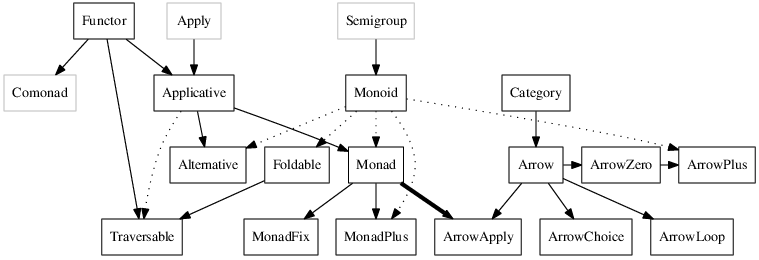
\includegraphics[scale=0.60000]{Typeclassopedia-diagram}\end{center}\end{changemargin}\newpage{}\section{Still for the curious: The Hask Category}In this section, we will dive in the \textbf{Hask} category, identifying some Haskell funcstions with their mathematical equivalent in Category Theory. Recalling from the first chapter:\begin{itemize}\item[$\mathfrak{Hask}$] : Obj($\mathfrak{Hask}$) -- the class of all Haskell types. Hom($\mathfrak{Hask}$) -- Haskell functions. The composition law is the $\mathtt{(.)}$ operator.\end{itemize}\subsection{Checking that \textbf{Hask} is a category}We can check the first and second law easily: we know \fbox{(.)} is an associative function, and clearly, for any \fbox{f} and \fbox{g}, \fbox{f . g} is another function. \par{}In Hask, the identity morphism is \fbox{id}, and we have trivially:\begin{verbatim}  id . f = f . id = f  
\end{verbatim}\par{}This isn't an exact translation of the law above, though; we're missing subscripts. The function \fbox{id} in Haskell is \textit{polymorphic}-- it can take many different types for its domain and range, or, in category-speak, can have many different source and target objects. But morphisms in category theory are by definition \textit{monomorphic}-- each morphism has one specific source object and one specific target object. A polymorphic Haskell function can be made monomorphic by specifying its type (\textit{instantiating} with a monomorphic type), so it would be more precise if we said that the identity morphism from \textbf{Hask} on a type \fbox{A} is \verb`(id :: A -> A)`. With this in mind, the above law would be rewritten as:\begin{verbatim}  (id :: B -> B) . f = f . (id :: A -> A) = f  
\end{verbatim} However, for simplicity, we will ignore this distinction when the meaning is clear.\par{}Actually, there is a subtlety here: because \fbox{(.)} is a lazy function, if \fbox{f} is \fbox{undefined}, we have that \verb`id . f = \_ -> `$\bot$ . Now, while this may seem equivalent to $\bot$ for all intents and purposes, you can actually tell them apart using the strictifying function \fbox{seq}, meaning that the last category law is broken. We can define a new strict composition function, \begin{verbatim}  f .! g = ((.) $! f) $! g   
\end{verbatim} that makes \textbf{Hask} a category. We proceed by using the normal \fbox{(.)}, though, and attribute any discrepancies to the fact that \fbox{seq} breaks an awful lot of the nice language properties anyway.\subsection{Functors on \textbf{Hask}}The Functor typeclass you have probably seen in Haskell does in fact tie in with the categorical notion of a functor. Remember that a functor has two parts: it maps objects in one category to objects in another and morphisms in the first category to morphisms in the second. Functors in Haskell are from \textbf{Hask} to \textit{func}, where \textit{func} is the subcategory of \textbf{Hask} defined on just that functor's types. E.g. the list functor goes from \textbf{Hask} to \textbf{Lst}, where \textbf{Lst} is the category containing only \textit{list types}, that is, \fbox{[T]} for any type \fbox{T}. The morphisms in \textbf{Lst} are functions defined on list types, that is, functions \verb`[T] -> [U]` for types \fbox{T}, \fbox{U}. How does this tie into the Haskell typeclass \fbox{Functor}? Recall its definition:\begin{verbatim}  class Functor (f :: * -> *) where  
    fmap :: (a -> b) -> f a -> f b  
\end{verbatim}\par{}Let's have a sample instance, too:\begin{verbatim}  instance Functor Maybe where  
    fmap f (Just x) = Just (f x)  
    fmap _ Nothing  = Nothing  
\end{verbatim}\par{}Here's the key part: the \textit{type constructor }\fbox{Maybe} takes any type \fbox{T} to a new type, \fbox{Maybe T}. Also, \fbox{fmap} restricted to Maybe types takes a function \verb`a -> b` to a function \verb`Maybe a -> Maybe b`. But that's it! We've defined two parts, something that takes objects in \textbf{Hask} to objects in another category (that of Maybe types and functions defined on Maybe types), and something that takes morphisms in \textbf{Hask} to morphisms in this category. So Maybe is a functor.\par{}A useful intuition regarding Haskell functors is that they represent types that can be mapped over. This could be a list or a Maybe, but also more complicated structures like trees. A function that does some mapping could be written using \fbox{fmap}, then any functor structure could be passed into this function. E.g. you could write a generic function that covers all of \fbox{Data.List.map}, \fbox{Data.Map.map}, \fbox{Data.Array.IArray.amap}, and so on.\par{}What about the functor axioms? The polymorphic function \fbox{id} takes the place of $id_{A}$ for any \fbox{A}, so the first law states:\begin{verbatim}  fmap id = id   
\end{verbatim}\par{}With our above intuition in mind, this states that mapping over a structure doing nothing to each element is equivalent to doing nothing overall. Secondly, morphism composition is just \fbox{(.)}, so \begin{verbatim}  fmap (f . g) = fmap f . fmap g   
\end{verbatim}This second law is very useful in practice. Picturing the functor as a list or similar container, the right-hand side is a two-pass algorithm: we map over the structure, performing \fbox{g}, then map over it again, performing \fbox{f}. The functor axioms guarantee we can transform this into a single-pass algorithm that performs \fbox{f . g}. This is a process known as \textit{fusion}.\subsubsection{Translating categorical concepts into Haskell}Functors provide a good example of how category theory gets translated into Haskell. The key points to remember are that:\begin{itemize}\item We work in the category \textbf{Hask} and its subcategories.\item Objects are types. \item Morphisms are functions. Things that take a type and return another type are type constructors. \item Things that take a function and return another function are higher-order functions.\item Typeclasses, along with the polymorphism they provide, make a nice way of capturing the fact that in category theory things are often defined over a number of objects at once.\end{itemize}\subsection{Monads}Monads are obviously an extremely important concept in Haskell, and in fact they originally came from category theory.\footnote{Experienced category theorists will notice that we're simplifying things a bit here; instead of presenting \textit{unit} and \textit{join} as natural transformations, we treat them explicitly as morphisms, and require naturality as extra axioms alongside the standard monad laws (laws 3 and 4). The reasoning is simplicity; we are not trying to teach category theory as a whole, simply give a categorical background to some of the structures in Haskell. You may also notice that we are giving these morphisms names suggestive of their Haskell analogues, because the names $\eta{}$ and $\mu{}$ don't provide much intuition.} A monad is a special type of functor, from a category to that same category, that supports some additional structure. So, down to definitions. A monad is a functor $M:C\to{} C$, along with two morphisms for every object X in C:\begin{itemize}\item ${{unit}_{X}}^{M}: X\to{}M(X)$\item ${{join}_{X}}^{M}M(M(X))\to{}M(X)$\end{itemize}When the monad under discussion is obvious, we'll leave out the ${ }^{M}$ superscript for these functions and just talk about ${unit}_{X}$ and ${join}_{X}$ for some $X$.\subsubsection{Translating}Let's see how this translates to the Haskell typeclass Monad, then.\begin{verbatim}  class Functor m => Monad m where   
    return :: a -> m a   
    (>>=)  :: m a -> (a -> m b) -> m b   
\end{verbatim}\par{}The class constraint of \fbox{Functor m} ensures that we already have the functor structure: a mapping of objects and of morphisms. \fbox{return} is the (polymorphic) analogue to ${unit}_{X}$ for any $X$. But we have a problem. \par{}Although \fbox{return}'s type looks quite similar to that of \textit{unit}; the other function, {\scriptsize{}\fbox{$(>>=)$}}, often called \textit{bind}, bears no resemblance to \textit{join}. There is however another monad function, \begin{verbatim}  join :: Monad m => m (m a) -> m a  
\end{verbatim} that looks quite similar. Indeed, we can recover \fbox{join} and {\scriptsize{}\fbox{$(>>=)$}} from each other:\begin{verbatim}  join :: Monad m => m (m a) -> m a  
  join x = x >>= id  
 
  (>>=) :: Monad m => m a -> (a -> m b) -> m b  
  x >>= f = join (fmap f x)  
\end{verbatim}So specifying a monad's \fbox{return}, \fbox{fmap},  and \fbox{join} is equivalent to specifying its \fbox{return}\fbox{fmap},  and {\scriptsize{}\fbox{$(>>=)$}}. It just turns out that the normal way of defining a monad in category theory is to give \fbox{unit} and \fbox{join}, whereas Haskell programmers like to give \fbox{return} and \fbox{bind.}\footnote{This is perhaps due to the fact that Haskell programmers like to think of monads as a way of sequencing computations with a common feature, whereas in category theory the container aspect of the various structures is emphasised. \fbox{join} pertains naturally to containers (squashing two layers of a container down into one), but {\scriptsize{}\fbox{$(>>=)$}} is the natural sequencing operation (do something, feeding its results into something else).} Often, the categorical way makes more sense. Any time you have some kind of structure \textit{M} and a natural way of taking any object $X$ into $M(X)$, as well as a way of taking $M(M(X))$ into $M(X)$, you probably have a monad. We can see this in the following example section.\subsubsection{Example: the powerset functor is also a monad}The power set functor $P:\mathbf{Set}\to{}\mathbf{Set}$ forms a monad. For any set $S$ you have a ${unit}_{S}(x)$ $=$ $\{x\}$, mapping elements to their singleton set. Note that each of these singleton sets are trivially a subset of $S$, so ${unit}_{S}$ returns elements of the powerset of $S$, as is required. Also, you can define a function ${join}_{S}$ as follows: we receive an input $L\in{}\mathcal{P}(\mathcal{P}(S))$. This is:\begin{itemize}\item A member of the powerset of the powerset of S.\item So a member of the set of all subsets of the set of all subsets of S.\item So a set of subsets of S.\end{itemize}We then return the union of these subsets, giving another subset of S. Symbolically, \begin{equation*}{join}_{S}(L)=\bigcup L\end{equation*}Hence $\mathcal{P}$ is a monad.\footnote{If you can prove that certain laws hold, which we'll explore with lists in the next subsection.}\par{}In fact, $\mathcal{P}$ is almost equivalent to the list monad; with the exception that we're talking lists instead of sets, they're almost the same. Compare:\begin{verbatim}
 \end{verbatim}\par{}Power set functor on \textbf{Set}, given a set $S$ and a morphism $f : A \to{}B$\begin{verbatim}
 \end{verbatim}\begin{center}\begin{tabular}{|c|c|}\hline \textbf{Function type}&\textbf{Definition}\\\hline $P(f) :\mathcal{P}(A)\to{}\mathcal{P}(B)$&$(P(f))(S)=\{f(a) : a\in{}S\}$\\\hline ${unit}_{S}: S\to{}\mathcal{P}(S)$&${unit}_{S}(x)=\{x\}$\\\hline ${join}_{S} : \mathcal{P}(\mathcal{P}(S))\to{}\mathcal{P}(S)$&${join}_{S}(L)=\bigcup L$\\\hline \end{tabular}\end{center}\begin{verbatim}
 
 \end{verbatim}\par{}List monad from Haskell, given a type \fbox{T} and a function \verb`f :: A -> B`\begin{verbatim}
 \end{verbatim}\begin{center}\begin{tabular}{|c|c|}\hline \textbf{Function type}&\textbf{Definition}\\\hline \verb`  fmap f :: [A] -> [B]  `&\verb`  fmap f xs = [ f a | a <- xs ]   `\\\hline \verb`  return :: T -> [T]  `&\verb`  return x = [x]  `\\\hline \verb`  join :: [[T]] -> [T]  `&\verb`  join xs = concat xs  `\\\hline \end{tabular}\end{center}\begin{verbatim}
 \end{verbatim}\subsection{The monad laws and their importance}Just as functors had to obey certain axioms in order to be called functors, monads have a few of their own. We'll first list them, then translate to Haskell, then see why they're important.\par{}Given a monad $M : C\to{}C$ and a morphism $f:A\to{}B$ for $A,B\in{}C$, \begin{enumerate}\item $join\circ{}M(join)=join\circ{}join$\item $join\circ{}M(unit)=join\circ{}unit=id$\item $unit\circ{}f=M(f)\circ{}unit$\item $join\circ{}M(M(f)=M(f)\circ{}join$\end{enumerate}\par{}By now, the Haskell translations should be hopefully self-explanatory:\begin{enumerate}\item \fbox{join . fmap join = join . join}\item \fbox{join . fmap return = join . return = id}\item \fbox{return . f = fmap f . return}\item \fbox{join . fmap (fmap f) = fmap f . join}\end{enumerate}\par{}(Remember that \fbox{fmap} is the part of a functor that acts on morphisms.) These laws seem a bit impenetrable at first, though. What on earth do these laws mean, and why should they be true for monads? Let's explore the laws.\subsubsection{The first law}\fbox{join . fmap join = join . join}\par{}In order to understand this law, we'll first use the example of lists. The first law mentions two functions, \fbox{join . fmap join} (the left-hand side) and \fbox{join . join} (the right-hand side). What will the types of these functions be? Remembering that \fbox{join}'s type is \verb`[[a]] -> [a]` (we're talking just about lists for now), the types are both \verb`[[[a]]] -> [a]` (the fact that they're the same is handy; after all, we're trying to show they're completely the same function!). So we have a list of lists of lists. The left-hand side, then, performs \fbox{fmap join} on this 3-layered list, then uses \fbox{join} on the result. \fbox{fmap} is just the familiar \fbox{map} for lists, so we first map across each of the list of lists inside the top-level list, concatenating them down into a list each. Now we have a list of lists, which we then run through \fbox{join}. In summary, we `enter' the top level, collapse the second and third levels down, then collapse this new level with the top level.\par{}What about the right-hand side? We first run \fbox{join} on our list of list of lists. Although this is three layers, and you normally apply a two-layered list to \fbox{join}, this will still work, because a \fbox{[[[a]]]} is just \fbox{[[b]]}, where \fbox{b = [a]}, so in a sense, a three-layered list is just a two layered list, but rather than the last layer being `flat', it is composed of another list. So if we apply our list of lists (of lists) to \fbox{join}, it will flatten those outer two layers into one. As the second layer wasn't flat but instead contained a third layer, we will still end up with a list of lists, which the other join flattens. Summing up, the left-hand side will flatten the inner two layers into a new layer, then flatten this with the outermost layer. The right-hand side will flatten the outer two layers, then flatten this with the innermost layer. These two operations should be equivalent. It's sort of like a law of associativity for \fbox{join}.\par{}\fbox{Maybe} is also a monad, with \begin{verbatim}  return :: a -> Maybe a  
  return x = Just x  
 
  join :: Maybe (Maybe a) -> Maybe a  
  join Nothing         = Nothing  
  join (Just Nothing)  = Nothing  
  join (Just (Just x)) = Just x  
\end{verbatim}So if we had a \textit{three}-layered Maybe (i.e., it could be \fbox{Nothing}, \fbox{Just Nothing}, \fbox{Just (Just Nothing)} or \fbox{Just (Just (Just x)))}, the first law says that collapsing the inner two layers first, then that with the outer layer is exactly the same as collapsing the outer layers first, then that with the innermost layer.\subsubsection{The second law}\fbox{join . fmap return = join . return = id}\par{}What about the second law, then? Again, we'll start with the example of lists. Both functions mentioned in the second law are functions \verb`[a] -> [a]`. The left-hand side expresses a function that maps over the list, turning each element \fbox{x} into its singleton list \fbox{[x]}, so that at the end we're left with a list of singleton lists. This two-layered list is flattened down into a single-layer list again using the \fbox{join}. The right hand side, however, takes the entire list \fbox{[x, y, z, ...]}, turns it into the singleton list of lists \fbox{[[x, y, z, ...]]}, then flattens the two layers down into one again. This law is less obvious to state quickly, but it essentially says that applying \fbox{return} to a monadic value, then \fbox{join}ing the result should have the same effect whether you perform the \fbox{return} from inside the top layer or from outside it.\subsubsection{The third and fourth laws}\fbox{return . f = fmap f . return}
 
\noindent{}\fbox{join . fmap (fmap f) = fmap f . join}\par{}The last two laws express more self evident fact about how we expect monads to behave. The easiest way to see how they are true is to expand them to use the expanded form:\begin{verbatim}1.   \x -> return (f x) = \x -> fmap f (return x)   
\end{verbatim}\begin{verbatim}2.   \x -> join (fmap (fmap f) x) = \x -> fmap f (join x)   
\end{verbatim}\subsubsection{Application to do-blocks}Well, we have intuitive statements about the laws that a monad must support, but why is that important? The answer becomes obvious when we consider do-blocks. Recall that a do-block is just syntactic sugar for a combination of statements involving {\scriptsize{}\fbox{$(>>=)$}} as witnessed by the usual translation:\begin{verbatim}  do { x }                 -->  x   
  do { let { y = v }; x }  -->  let y = v in do { x }   
  do { v <- y; x }         -->  y >>= \v -> do { x }   
  do { y; x }              -->  y >>= \_ -> do { x }   
\end{verbatim}\par{}Also notice that we can prove what are normally quoted as the monad laws using \fbox{return} and {\scriptsize{}\fbox{$(>>=)$}} from our above laws (the proofs are a little heavy in some cases, feel free to skip them if you want to):\begin{verbatim}1.  return x >>= f = f x   -- First Law 
\end{verbatim}\par{}Proof:\begin{verbatim}     return x >>= f   
   = join (fmap f (return x)) -- By the definition of (>>=)   
   = join (return (f x))      -- By law 3   
   = (join . return) (f x)   
   = id (f x)                 -- By law 2   
   = f x   
 
\end{verbatim}\begin{verbatim}2.  m >>= return = m   -- Second Law 
\end{verbatim}\par{}Proof:\begin{verbatim}    m >>= return   
   = join (fmap return m)    -- By the definition of (>>=)   
   = (join . fmap return) m   
   = id m                    -- By law 2   
   = m   
 
\end{verbatim}\begin{verbatim}3.  (m >>= f) >>= g = m >>= (\x -> f x >>= g)\end{verbatim}\par{}Proof (recall that \fbox{fmap f . fmap g = fmap (f . g)}):\begin{verbatim}    (m >>= f) >>= g                                                                               
  = (join (fmap f m)) >>= g                          -- By the definition of (>>=)             
  = join (fmap g (join (fmap f m)))                  -- By the definition of (>>=)             
  = (join . fmap g) (join (fmap f m))                                                          
  = (join . fmap g . join) (fmap f m)                                                          
  = (join . join . fmap (fmap g)) (fmap f m)         -- By law 4                               
  = (join . join . fmap (fmap g) . fmap f) m                                                   
  = (join . join . fmap (fmap g . f)) m              -- By the distributive law of functors    
  = (join . join . fmap (\x -> fmap g (f x))) m                                               
  = (join . fmap join . fmap (\x -> fmap g (f x))) m -- By law 1                              
  = (join . fmap (join . (\x -> fmap g (f x)))) m    -- By the distributive law of functors   
  = (join . fmap (\x -> join (fmap g (f x)))) m                                               
  = (join . fmap (\x -> f x >>= g)) m                -- By the definition of (>>=)            
  = join (fmap (\x -> f x >>= g) m)                                                           
  = m >>= (\x -> f x >>= g)                          -- By the definition of (>>=)            
\end{verbatim}\par{}These new monad laws, using \fbox{return} and {\scriptsize{}\fbox{$(>>=)$}}, can be translated into do-block notation.\begin{verbatim}
 \end{verbatim}\begin{center}\begin{tabular}{|c|c|}\hline \textbf{Points-free style}&\textbf{Do-block style}\\\hline \verb`  return x >>= f = f x  `&\verb`  do { v <- return x; f v } = do { f x }  `\\\hline \verb`  m >>= return = m  `&\verb`  do { v <- m; return v } = do { m }  `\\\hline \verb`  (m >>= f) >>= g = m >>= (\x -> f x >>= g)  `&\begin{minipage}{6cm}\begin{verbatim}  do { y <- do { x <- m; f x }; g y}  
= 
  do { x <- m; y <- f x; g y } \end{verbatim}\end{minipage}\\\hline \end{tabular}\end{center}\begin{verbatim}
 \end{verbatim}The monad laws are now common-sense statements about how do-blocks should function. If one of these laws were invalidated, users would become confused, as you couldn't be able to manipulate things within the do-blocks as would be expected. The monad laws are, in essence, usability guidelines.\appendix{}\chapter{Appendix: The fundamental groupoid}NOT directly RELATED TO MONAD\paragraph{ }Let X be a topological space. We define a category $\Pi(X)$ (which will turn out to be a groupoid) as follows.\begin{itemize}\item  The objects of $\Pi(X)$ are the points of X. \end{itemize}

 In order to define morphisms in $\Pi(X)$ we need to recall the notion of \textit{homotopy of paths}. Suppose $x,y\in{}X$ and ${\gamma{}}_{0},{\gamma{}}_{1}$ : $[0,1]\to{}X$ are continous maps (where the closed interval [0,1] is equipped with the usual topology) such that ${\gamma{}}_{0}(0) = x = {\gamma{}}_{1}(0)$ and ${\gamma{}}_{0}(1) = y = {\gamma{}}_{1}(1)$. (One can say that ${\gamma{}}_{0}$ and ${\gamma{}}_{1}$ are (continous) paths from x to y).

 We say that ${\gamma{}}_{0}$ and ${\gamma{}}_{1}$ are \textbf{homotopic} if there exists a continous map $H : [0,1]\times{}[0,1]\to{}X$, called a \textbf{homotopy} between ${\gamma{}}_{0}$ and ${\gamma{}}_{1}$, such that $H(t,0)={\gamma{}}_{0}(t)$ and $H(t,1)={\gamma{}}_{1}(t)$, $\forall{}t\in{}[0,1]$, and also $H(0,s)=x$ and $H(1,s)=y$, $\forall{}s\in{}[0,1]$. Observe that these conditions can be rephrased as follows. If we define ${H}_{s}(t)=H(t,s)$, then, for every fixed $s\in{}[0,1]$, ${H}_{s}$ should be a (continous) path from x to y, and, moreover, one should have ${H}_{0}={\gamma{}}_{0}$ and ${H}_{1}={\gamma{}}_{1}$.

 Check that being homotopic is an equivalence relation on continuous paths from x to y. This allows us to define, for every pair $x,y\in{}X$, the set of equivalence classes of continuous paths from x to y modulo homotopy.\begin{itemize}\item For two objects \textit{x, y} of $\Pi(X)$, we define ${Hom}_{\Pi(X)}(x, y)$ to be the set of homotopy classes of continuous paths from \textit{x} to \textit{y}.\end{itemize}Finally, we need to define composition of paths. If $\alpha{}$ : $[0,1]\to{} X $ and $\beta{}$ : $[0,1]\to{} Y $ are continuous maps such that $\alpha{}(1)=\beta{}(0)$, we can define a continuous map\begin{equation*}\beta{}\cdot{}\alpha{} : [0,1]\to{}X;\qquad{}t\mapsto{}\begin{cases} \alpha (2t), & \mbox{if } 0\leq t\leq \frac{1}{2} \\ \beta (2t-1) , & \mbox{if } \frac{1}{2}\leq t\leq 1 \end{cases}\end{equation*}Check that composition of paths respects homotopy. In other words, if ${\alpha{}}_{0}$ , ${\alpha{}}_{1}$ are two homotopic paths from $x\to{}y$, and ${\beta{}}_{0}$ , ${\beta{}}_{1}$ are two homotopic paths from $y\to{}z$, then the paths ${\beta{}}_{0}\cdot{}{\alpha{}}_{0}$ and ${\beta{}}_{1}\cdot{}{\alpha{}}_{0}$ from $x\to{}z$ are also homotopic.\begin{itemize}\item This allows us to define composition of morphisms in $\Pi(X)$ unambiguously: if $x,y,z\in{}X$, then to define the composition map\begin{equation*}Hom(y, z)\times{}Hom(x, y)\to{}Hom(x, z)\end{equation*}let us pick equivalence classes $f\in{}Hom(x, y)$ , $g\in{}Hom(y, z)$ and representatives $\alpha{}$ : $[0,1]\to{}X$, $\beta{}$ : $[0,1]\to{}X$ of $f$ and $g$, respectively. Then we define $g\circ{}f$ to be the equivalence class of $\beta{}\cdot{}\alpha{}$.\end{itemize}\begin{prop}Verify the following statements:\begin{enumerate}\item Composition of homotopy classes of continuous paths is associative. (There is something to think about, because composition of continuous paths, before passing to homotopy classes, is NOT associative!)\item The definitions above turn $\Pi(X)$ into a category.\item $\Pi(X)$ is in fact a groupoid. Indeed, if $f$ : $x\to{}y$ is a morphism in $\Pi(X)$ and $\alpha{}$ : $[0,1]\to{}X$ is a representative of f, as before, check that the equivalence class of the path ${\alpha{}}^{-1} : [0,1]\to{}X$ defined by ${\alpha{}}^{-1}(t)=\alpha{}(1-t)$ is an inverse of f.\end{enumerate}\end{prop}\paragraph{\textit{Def:}}One calls $\Pi(X)$ the \textbf{fundamental groupoid} of the topological space $X$. If we fix a point $x\in{}X$, then, in particular, all morphisms from $x$ to $x$ in $\Pi(X)$ form a group which we denote ${Aut}_{\Pi(X)}(x)$. In topology it has a diferent name: the \textit{fundamental group of X at the point x} is defined to be \begin{equation*}{\pi{}}_{1}(X,x):={Aut}_{\Pi(X)}(x)\end{equation*}Check that this definition of the fundamental group is equivalent to the other one(s) you have seen. The proof will be essentially tautological. The definition of the fundamental groupoid is no more complicated than the definition of the fundamental group; however, for many purposes it is much more convenient to think in terms of the fundamental groupoid rather than the fundamental group.\paragraph{ }For example, the definition of the fundamental groupoid is completely canonical, while the definition of the fundamental group depends on the choice of a base point. In particular, if $X$ has several connected components, then $\Pi(X)$ ``keeps track'' of all of them, while if we choose a base point $x\in{}X$, then ${\pi{}}_{1}(X,x)$ does not know anything about the connected components of $X$ that do not contain $x$. For instance, if $X$ is the disjoint union of a circle and a line, and $x\in{}X$ is a point lying on the line, then ${\pi{}}_{1}(X,x)$ is the trivial group, while $\Pi(X)$ looks like the ``disjoint union'' (you can try to think how to define the disjoint union of two categories in general - this is not dificult) of the fundamental groupoid of a circle and the fundamental groupoid of a line.\chapter{Appendix: Full Monad documentation}The full \fbox{Monad} code, as found in the Prelude documentation when searching "Monad" in Hoogle\begin{verbatim}{- | The 'Monad' class defines the basic operations over a /monad/, 
 a concept from a branch of mathematics known as /category theory/. 
 From the perspective of a Haskell programmer, however, it is best to 
 think of a monad as an /abstract datatype/ of actions. 
 Haskell's @do@ expressions provide a convenient syntax for writing 
 monadic expressions. 
 
 Instances of 'Monad' should satisfy the following laws: 
 
 * @'return' a '>>=' k  =  k a@ 
 * @m '>>=' 'return'  =  m@ 
 * @m '>>=' (\x -> k x '>>=' h)  =  (m '>>=' k) '>>=' h@ 
 
 Furthermore, the 'Monad' and 'Applicative' operations should relate as follows: 
 
 * @'pure' = 'return'@ 
 * @('<*>') = 'ap'@ 
 
 The above laws imply: 
 
 * @'fmap' f xs  =  xs '>>=' 'return' . f@ 
 * @('>>') = ('*>')@ 
 
 and that 'pure' and ('<*>') satisfy the applicative functor laws. 
 
 The instances of 'Monad' for lists, 'Data.Maybe.Maybe' and 'System.IO.IO' 
 defined in the "Prelude" satisfy these laws. 
 -}  
 class Applicative m => Monad m where 
     -- | Sequentially compose two actions, passing any value produced 
     -- by the first as an argument to the second. 
     (>>=)       :: forall a b. m a -> (a -> m b) -> m b 
 
     -- | Sequentially compose two actions, discarding any value produced 
     -- by the first, like sequencing operators (such as the semicolon) 
     -- in imperative languages. 
     (>>)        :: forall a b. m a -> m b -> m b 
     m >> k = m >>= \_ -> k -- See Note [Recursive bindings for Applicative/Monad] 
     {-# INLINE (>>) #-} 
 
     -- | Inject a value into the monadic type. 
     return      :: a -> m a 
     return      = pure 
 
     -- | Fail with a message.  This operation is not part of the 
     -- mathematical definition of a monad, but is invoked on pattern-match 
     -- failure in a @do@ expression. 
     fail        :: String -> m a 
     fail s      = error s 
 
 {- Note [Recursive bindings for Applicative/Monad] 
 ~~~~~~~~~~~~~~~~~~~~~~~~~~~~~~~~~~~~~~~~~~~~~~~~~~  
 
 The original Applicative/Monad proposal stated that after 
 implementation, the designated implementation of (>>) would become 
 
   (>>) :: forall a b. m a -> m b -> m b 
   (>>) = (*>) 
 
 by default. You might be inclined to change this to reflect the stated 
 proposal, but you really shouldn't! Why? Because people tend to define 
 such instances the /other/ way around: in particular, it is perfectly 
 legitimate to define an instance of Applicative (*>) in terms of (>>), 
 which would lead to an infinite loop for the default implementation of 
 Monad! And people do this in the wild. 
 
 This turned into a nasty bug that was tricky to track down, and rather 
 than eliminate it everywhere upstream, it's easier to just retain the 
 original default. 
 
 -}\end{verbatim}\chapter{Appendix: the Monoid type class}Not to be confused with the Monad class, the more pleasant Monoid class, with kind \verb` * -> Constraint `, found in the \fbox{Data.Monoid} module, modelizes the semigroups or monoids.\par{}A \textbf{monoid} in Mathematics is an algebraic structure consisting of a set of objects with an operation between them, being this operation \textit{associative} and with a \textit{neutral element}.  Phew! But what is the meaning of this? By \textit{associative} we mean that, if you have three elements $a$, $b$ and $c$, then $a*(b*c) = (a*b)*c$. A \textit{neutral element} is the one that does not worth to operate with, because it does nothing! To say, $e$ is a \textit{neutral element} if $e*a = a*e = a$, given any object $a$. As an example, you may take the real numbers as objects and the ordinary multiplication as operation.\par{}Now that you know the math basics behind the Monoid class, let's see its definition:\begin{verbatim}  class Monoid m where 
     mempty :: m 
     mappend :: m -> m -> m 
     mconcat :: [m] -> m 
     mconcat = foldr mappend mempty 
     (<>) :: m -> m -> m    -- infix synonym for mappend \end{verbatim}\par{}See that \textbf{mappend} corresponds to the monoid operation and \textbf{mempty} to its neutral element. The names of the methods may seem unsuitable, but they correspond to an example of monoid: the lists with the appending \verb`(++)` operation. Who is the neutral element here? The empty list:\begin{verbatim}    xs ++ [] = [] ++ xs = xs\end{verbatim}\par{}Some examples:\newpage{}\par{}The list monoid\begin{verbatim}instance Monoid [a] where  
         mempty  = [] 
         mappend = (++) 
         mconcat xss = [x | xs <- xss, x <- xs] 
 \end{verbatim}\par{}The monoid of functions with range a monoid\begin{verbatim}instance Monoid b => Monoid (a -> b) where 
         mempty _ = mempty 
         mappend f g x = f x `mappend` g x 
 \end{verbatim}\par{}The Unit monoid\begin{verbatim}instance Monoid () where 
         mempty        = () 
         _ `mappend` _ = () 
         mconcat _     = () 
 \end{verbatim}\par{}The cartesian product of two monoids\begin{verbatim}instance (Monoid a, Monoid b) => Monoid (a,b) where 
         mempty = (mempty, mempty) 
         (a1,b1) `mappend` (a2,b2) = 
                 (a1 `mappend` a2, b1 `mappend` b2) 
 \end{verbatim}\par{}Lexicographical ordering\begin{verbatim}instance Monoid Ordering where 
         mempty         = EQ 
         LT `mappend` _ = LT 
         EQ `mappend` y = y 
         GT `mappend` _ = GT 
 \end{verbatim}\par{}Lift a semigroup into `Maybe' forming a `Monoid'\begin{verbatim}instance Monoid a => Monoid (Maybe a) where 
   mempty = Nothing 
   Nothing `mappend` m = m 
   m `mappend` Nothing = m 
   Just m1 `mappend` Just m2 = Just (m1 `mappend` m2) 
\end{verbatim}\par{}As you can see in all the examples, the following rules are verified:\begin{verbatim}  (x <> y) <> z = x <> (y <> z)   -- associativity 
  mempty <> x = x                 -- left identity 
  x <> mempty = x                 -- right identity 
\end{verbatim}\chapter{Appendix: the Maybe monad}We introduced monads using \fbox{Maybe} as an example. The \fbox{Maybe} monad represents computations which might ``go wrong'' by not returning a value. For reference, here are our definitions of \fbox{return} and {\scriptsize{}\fbox{$(>>=)$}} for \fbox{Maybe} as we saw in the main body:\footnote{The definitions in the actual instance in \fbox{Data.Maybe} are written a little differently, but are fully equivalent to these. }\begin{verbatim}    return :: a -> Maybe a 
    return x  = Just x 

    (>>=)  :: Maybe a -> (a -> Maybe b) -> Maybe b 
    m >>= g = case m of 
                 Nothing -> Nothing 
                 Just x  -> g x 
\end{verbatim}\section{Safe functions}The \fbox{Maybe} datatype provides a way to make a safety wrapper around \textit{partial functions}, that is, functions which can fail to work for a range of arguments. For example, \fbox{head} and \fbox{tail} only work with non-empty lists. Another typical case, which we will explore in this section, are mathematical functions like \fbox{sqrt} and \fbox{log}; (as far as real numbers are concerned) these are only defined for non-negative arguments.\begin{verbatim} > log 1000 
 6.907755278982137 
 > log (-1000) 
 ''ERROR'' -- runtime error 
\end{verbatim}To avoid this crash, a ``safe'' implementation of log could be:\begin{verbatim} safeLog :: (Floating a, Ord a) => a -> Maybe a 
 safeLog x 
     | x > 0    = Just (log x) 
     | otherwise = Nothing 
\end{verbatim}\begin{verbatim} > safeLog 1000 
 Just 6.907755278982137 
 > safeLog -1000 
 Nothing 
\end{verbatim}We could write similar ``safe functions'' for all functions with limited domains such as division, square-root, and inverse trigonometric functions (\fbox{safeDiv}, \fbox{safeSqrt}, \fbox{safeArcSin}, etc. all of which would have the same \textit{type} as \fbox{safeLog} but definitions specific to their constraints)\par{}If we wanted to combine these monadic functions, the cleanest approach is with monadic composition and point-free style:\begin{verbatim} safeLogSqrt = safeLog <=< safeSqrt \end{verbatim}Written in this way, \fbox{safeLogSqrt} resembles a lot its unsafe, non-monadic counterpart:\begin{verbatim} unsafeLogSqrt = log . sqrt \end{verbatim}\section{Lookup tables}A lookup table relates \textit{keys} to \textit{values}. You look up a value by knowing its key and using the lookup table. For example, you might have a phone book application with a lookup table where contact names are keys to corresponding phone numbers.
 An elementary way of implementing lookup tables in Haskell is to use a list of pairs: \fbox{[(a, b)]}. Here \fbox{a} is the type of the keys, and \fbox{b} the type of the values.\footnote{ Check \fbox{Data.Map} for a different, and potentially more useful, implementation.}Here's how the phone book lookup table might look like:\begin{verbatim} phonebook :: [(String, String)] 
 phonebook = [ (`Bob',   `01788 665242'), 
               (`Fred',  `01624 556442'), 
               (`Alice', `01889 985333'), 
               (`Jane',  `01732 187565') ] 
\end{verbatim}The most common thing you might do with a lookup table is look up values. Everything is fine if we try to look up ``Bob'', ``Fred'', ``Alice'' or ``Jane'' in our phone book, but what if we were to look up ``Zoe''? 
Zoe isn't in our phone book, so the lookup would fail. Hence, the Haskell function to look up a value from the table is a \fbox{Maybe} computation (it is available from Prelude): \begin{verbatim} lookup :: Eq a => a  -- a key 
        -> [(a, b)]   -- the lookup table to use 
        -> Maybe b    -- the result of the lookup 
\end{verbatim}Let us explore some of the results from lookup:\begin{verbatim} Prelude> lookup `Bob' phonebook 
 Just `01788 665242' 
 Prelude> lookup `Jane' phonebook 
 Just `01732 187565' 
 Prelude> lookup `Zoe' phonebook 
 Nothing 
\end{verbatim}Now let's expand this into using the full power of the monadic interface. Say, we're now working for the government, and once we have a phone number from our contact, we want to look up this phone number in a big, government-sized lookup table to find out the registration number of their car. This, of course, will be another \fbox{Maybe}-computation. But if the person we're looking for isn't in our phone book, we certainly won't be able to look up their registration number in the governmental database.\par{}What we need is a function that will take the results from the first computation and put it into the second lookup \textit{only} if we get a successful value in the first lookup. Of course, our final result should be \fbox{Nothing} if we get \fbox{Nothing} from either of the lookups.\begin{verbatim} getRegistrationNumber :: String       -- their name 
                       -> Maybe String -- their Reg.Num. 
 getRegistrationNumber name =  
   lookup name phonebook >>= 
     (\number -> lookup number governmentDatabase) 
\end{verbatim}If we then wanted to use the result from the governmental database lookup in a third lookup (say we want to look up their registration number to see if they owe any car tax), then we could extend our \fbox{getRegistrationNumber} function:\begin{verbatim} getTaxOwed :: String       -- their name 
           -> Maybe Double -- the amount of tax they owe 
 getTaxOwed name =  
   lookup name phonebook >>= 
     (\number -> lookup number governmentDatabase) >>= 
       (\registration -> lookup registration taxDatabase) 
\end{verbatim}Or, using the \fbox{do}-block style:\begin{verbatim} getTaxOwed name = do 
   number       <- lookup name phonebook 
   registration <- lookup number governmentDatabase 
   lookup registration taxDatabase 
\end{verbatim}Let's just pause here and think about what would happen if we got a \fbox{Nothing} anywhere. By definition, when the first argument to {\scriptsize{}\fbox{$(>>=)$}} is \fbox{Nothing}, it just returns \fbox{Nothing} while ignoring whatever function it is given. Thus, a \fbox{Nothing} at any stage in the large computation will result in a \fbox{Nothing} overall, regardless of the other functions. After the first \fbox{Nothing} hits, all {\scriptsize{}\fbox{$(>>=)$}}s will just pass it to each other, skipping the other function arguments. The technical description says that the structure of the \fbox{Maybe} monad \textbf{propagates failures}.\section{Open monads}Another trait of the \fbox{Maybe} monad is that it is \textbf{open}: if we have a \fbox{Just} value, we can see the contents and extract the associated values through pattern matching.\begin{verbatim} zeroAsDefault :: Maybe Int -> Int 
 zeroAsDefault mx = case mx of 
     Nothing -> 0 
     Just x -> x 
\end{verbatim}This usage pattern of replacing \fbox{Nothing} with a default is captured by the \fbox{fromMaybe} function in \fbox{Data.Maybe}.\begin{verbatim} zeroAsDefault :: Maybe Int -> Int 
 zeroAsDefault mx = fromMaybe 0 mx 
\end{verbatim}The \fbox{maybe} Prelude function allows us to do it in a more general way, by supplying a function to modify the extracted value.\begin{verbatim} displayResult :: Maybe Int -> String 
 displayResult mx = maybe s1 ((s2++).show) mx 
   where 
     s1 = `There was no result' 
     s2 = `The result was'  
 
\end{verbatim}\begin{verbatim} Prelude> :t maybe 
 maybe :: b -> (a -> b) -> Maybe a -> b 
 Prelude> displayResult (Just 10) 
 `The result was 10' 
 Prelude> displayResult Nothing 
 `There was no result' 
\end{verbatim}This possibility makes sense for \fbox{Maybe}, as it allows us to recover from failures. Not all monads are open in this way; often, they are designed to hide unnecessary details. \fbox{return} and {\scriptsize{}\fbox{$(>>=)$}} alone do not allow us to extract the underlying value from a monadic computation, and so it is perfectly possible to make a ``no-exit'' monad, from which it is never possible to extract values. The most obvious example of that is the \fbox{IO} monad.\section{Maybe and safety}We have seen how \fbox{Maybe} can make code safer by providing a graceful way to deal with failure that does not involve runtime errors. Does that mean we should always use \fbox{Maybe} for everything? Not really.\par{}When you write a function, you are able to tell whether it might fail to produce a result during normal operation of the program\footnote{With ``normal operation'' we mean to exclude failure caused by uncontrollable circumstances in the real world, such as memory exhaustion or a dog chewing the printer cable. }, either because the functions you use might fail (as in the examples in this chapter) or because you know some of the argument or intermediate result values do not make sense (for instance, imagine a calculation that is only meaningful if its argument is less than 10). If that is the case, by all means use \fbox{Maybe} to signal failure; it is far better than returning an arbitrary default value or throwing an error.\par{}Now, adding \fbox{Maybe} to a result type without a reason would only make the code more confusing and no safer. The type signature of a function with unnecessary \fbox{Maybe} would tell users of the code that the function could fail when it actually can't.
 Of course, that is not as bad a lie as the opposite one (that is, claiming that a function will not fail when it actually can), but we really want honest code in \textit{all} cases. Furthermore, using \fbox{Maybe} forces us to propagate failure (with \fbox{fmap} or monadic code) and eventually handle the failure cases (using pattern matching, the \fbox{maybe} function, or \fbox{fromMaybe} from \fbox{Data.Maybe}). If the function cannot actually fail, coding for failure is an unnecessary complication.\chapter{Appendix: The List monad}Lists are a fundamental part of Haskell, and we've used them extensively before getting to this chapter. The novel insight is that the list type is a monad too!\par{}As monads, lists are used to model \textit{nondeterministic} computations which may return an arbitrary number of results. There is a certain parallel with how \fbox{Maybe} represented computations which could return zero or one value; but with lists, we can return zero, one, or many values (the number of values being reflected in the length of the list).\section{List instantiated as monad}The \fbox{return} function for lists simply injects a value into a list:\begin{verbatim}  return x  =  [x] 
\end{verbatim}In other words, \fbox{return} here makes a list containing one element, namely the single argument it took. The type of the \textit{list return} is \fbox{return :: $a \to{} [a]$}, or, equivalently, \fbox{return :: $a \to{}[\,]\:a$}. The latter style of writing it makes it more obvious that we are replacing the generic type constructor (which we had called \fbox{M} in Understanding monads) by the list type constructor \fbox{[ ]} (which is distinct from but easy to confuse with the empty list!).\par{}The binding operator is less trivial. We will begin by considering its type, which for the case of lists should be:\begin{verbatim}  [a] -> (a -> [b]) -> [b] 
\end{verbatim}This is just what we'd expect: it pulls out the value from the list to give to a function that returns a new list.\par{}The actual process here involves first mapping a given function over a given list to get back a list of lists, i.e. type \fbox{[[b]]} (of course, many functions which you might use in mapping do not return lists; but, as shown in the type signature above, \textbf{monadic binding for lists only works with functions that return lists}). To get back to a regular list, we then concatenate the elements of our list of lists to get a final result of type \fbox{[b]}. Thus, we can define the list version of {\scriptsize{}\fbox{$(>>=)$}}:\begin{verbatim}  xs >>= f = concat (map f xs) 
\end{verbatim}The bind operator is key to understanding how different monads do their jobs, and its definition indicates the chaining strategy for working with the monad.\par{}For the list monad, non-determinism is present because different functions may return any number of different results when mapped over lists.\subsubsection{Bunny invasion}\begin{verbatim}  Prelude> let generation = replicate 2             
  Prelude> ['bunny'] >>= generation                  
  ['bunny','bunny']                                  
  Prelude> ['bunny'] >>= generation >>= generation   
  ['bunny','bunny','bunny','bunny']                  
\end{verbatim}In this silly example all elements are equal, but the same overall logic could be used to model radioactive decay, or chemical reactions, or any phenomena that produces a series of elements starting from a single one.\section{Board game example}Suppose we are modeling a turn-based board game and want to find all the possible ways the game could progress. We would need a function to calculate the list of options for the next turn, given a current board state:\begin{verbatim}  nextConfigs :: Board -> [Board]                     
  nextConfigs bd = undefined -- details not important  
\end{verbatim}To figure out all the possibilities after two turns, we would again apply our function to each of the elements of our new list of board states. Our function takes a single board state and returns a list of possible new states. Thus, we can use monadic binding to map the function over each element from the list:\begin{verbatim}  nextConfigs bd >>= nextConfigs\end{verbatim}In the same fashion, we could bind the result back to the function yet again (ad infinitum) to generate the next turn's possibilities. Depending on the particular game's rules, we may reach board states that have no possible next-turns; in those cases, our function will return the empty list.\par{}On a side note, we could translate several turns into a do block (like we did for the grandparents example in Understanding monads):\begin{verbatim}  threeTurns :: Board -> [Board]  
  threeTurns bd = do           
    bd1 <- nextConfigs bd      
    bd2 <- nextConfigs bd1     
    nextConfigs bd2            
\end{verbatim}If the above looks too magical, keep in mind that \fbox{do} notation is syntactic sugar for {\scriptsize{}\fbox{$(>>=)$}} operations. To the right of each left-arrow, there is a function with arguments that evaluate to a list; the variable to the left of the arrow stands for the list elements. 
 After a left-arrow assignment line, there can be later lines that call the assigned variable as an argument for a function. This later function will be performed for \textit{each} of the elements from within the list that came from the left-arrow line's function. This per-element process corresponds to the `map' in the definition of {\scriptsize{}\fbox{$(>>=)$}}. A resulting list of lists (one per element of the original list) will be flattened into a single list (the `concat' in the definition of {\scriptsize{}\fbox{$(>>=)$}}).\section{List comprehensions}The list monad works in a way that has uncanny similarity to list comprehensions. Let's slightly modify the \fbox{do} block we just wrote for \fbox{threeTurns} so that it ends with a \fbox{return}...\begin{verbatim}  threeTurns bd = do          
    bd1 <- nextConfigs bd  
    bd2 <- nextConfigs bd1 
    bd3 <- nextConfigs bd2 
    return bd3             
\end{verbatim}This mirrors exactly the following list comprehension:\begin{verbatim}threeTurns bd = 
  [ bd3 | bd1 <- nextConfigs bd, bd2 <- nextConfigs bd1, bd3 <- nextConfigs bd2 ]\end{verbatim}(In a list comprehension, it is perfectly legal to use the elements drawn from one list to define the following ones, like we did here.)\par{}The resemblance is no coincidence: list comprehensions are, behind the scenes, defined in terms of \fbox{concatMap}\begin{verbatim}  concatMap f xs = concat (map f xs)  \end{verbatim}. That's just the list monad binding definition again! To summarize the nature of the list monad: binding for the list monad is a combination of concatenation and mapping, and so the combined function \fbox{concatMap} is effectively the same as {\scriptsize{}\fbox{$(>>=)$}} for lists (except for different syntactic order).\par{}For the correspondence between list monad and list comprehension to be complete, we need a way to reproduce the filtering that list comprehensions can do. Search for Additive Monads (MonadPlus).\chapter{Appendix: The IO (Input/Output) monad}Haskell is a \textit{functional} and \textit{lazy} language. However, the real world effects of input/output operations can't be expressed through pure functions. Furthermore, in most cases I/O can't be done lazily. Since lazy computations are only performed when their values become necessary, unfettered lazy I/O would make the order of execution of the real world effects unpredictable. Haskell addresses these issues through the \fbox{IO} monad.\section{Input/output and purity}Haskell functions are \textit{pure}: when given the same arguments, they return the same results. Pure functions are reliable and predictable; they ease debugging and validation. Test cases can also be set up easily since we can be sure that nothing other than the arguments will influence a function's result. Being entirely contained within the program, the Haskell compiler can evaluate functions thoroughly in order to optimize the compiled code.\par{}So, how do we manage actions like opening a network connection, writing a file, reading input from the outside world, or anything else that does something more than returning a calculated result? Well, the key is: \textit{these actions are not functions}. The \fbox{IO} monad is a means to represent actions as Haskell values, so that we can manipulate them with pure functions.\section{Combining functions and I/O actions}Let's combine functions with I/O to create a full program that will:\begin{enumerate}\item Ask the user to insert a string\item Read their string\item Use \fbox{fmap} to apply a function \fbox{shout} that capitalizes all the letters from the string\item Write the resulting string\end{enumerate}\begin{verbatim}  module Main where 
 
  import Data.Char (toUpper) 
  import Control.Monad 
 
  main = putStrLn "Write your string: " >> fmap shout getLine >>= putStrLn 
 
  shout = map toUpper 
 
\end{verbatim}We have a full-blown program, but we didn't include any type definitions. Which parts are functions and which are IO actions or other values? We can load our program in GHCi and check the types:\begin{verbatim}  main :: IO ()                                       
  putStrLn :: String -> IO ()                      
  "Write your string: " :: [Char]  
  (>>) :: Monad m => m a -> m b -> m b             
  fmap :: Functor m => (a -> b) -> m a -> m b      
  shout :: [Char] -> [Char]                        
  getLine :: IO String                             
  (>>=) :: Monad m => m a -> (a -> m b) -> m b     
\end{verbatim}\par{}Whew, that is a lot of information there. We've seen all of this before, but let's review.\par{}\fbox{main} is \fbox{IO ()}. That's not a function. Functions are of types \fbox{$ a \to{} b $}. Our entire program is an IO action.\par{}\fbox{putStrLn} is a function, but it results in an IO action. The ``Write your string:'' text is a \fbox{String} (remember, that's just a synonym for \fbox{[Char]}). It is used as an argument for \fbox{putStrLn} and is incorporated into the IO action that results. So, \fbox{putStrLn} is a function, but \fbox{putStrLn x} evaluates to an IO action. The \fbox{()} part of the IO type indicates that nothing is available to be passed on to any later functions or actions.That last part is key. We sometimes say informally that an IO action ``returns'' something; however, taking that too literally leads to confusion. It is clear what we mean when we talk about \textit{functions} returning results, but IO actions are not functions. Let's skip down to \fbox{getLine} - an IO action that \textit{does} provide a value. \fbox{getLine} is not a function that returns a \fbox{String} because \fbox{getLine}\textit{ isn't a function}. Rather, \fbox{getLine} is an IO action which, when evaluated, will materialize a \fbox{String}, which can then be passed to later functions through, for instance, \fbox{fmap} and {\scriptsize{}\fbox{$(>>=)$}}.When we use \fbox{getLine} to get a \fbox{String}, the value is monadic because it is wrapped in \fbox{IO} functor (which happens to be a monad). We cannot pass the value directly to a function that takes plain (non-monadic, or non-functorial) values. \fbox{fmap} does the work of taking a non-monadic function while passing in and returning monadic values. \par{}As we've seen already, {\scriptsize{}\fbox{$(>>=)$}} does the work of passing a monadic value into a function that takes a non-monadic value and returns a monadic value. It may seem inefficient for \fbox{fmap} to take the non-monadic result of its given function and return a monadic value only for {\scriptsize{}\fbox{$(>>=)$}} to then pass the underlying non-monadic value to the next function. It is precisely this sort of chaining, however, that creates the reliable sequencing that make monads so effective at integrating pure functions with IO actions. \subsubsection{\textit{do} notation review}Given the emphasis on sequencing, the \fbox{do} notation can be especially appealing with the \fbox{IO} monad. Our program \begin{verbatim}  putStrLn "Write your string: " >> fmap shout getLine >>= putStrLn 
 \end{verbatim}could be written as:\begin{verbatim}  do putStrLn "Write your string: "  
     string <- getLine                            
     putStrLn (shout string)                      
\end{verbatim}\section{The universe as part of our program}One way of viewing the \fbox{IO} monad is to consider \fbox{IO a} as a computation which provides a value of type \fbox{a} while changing \textit{the state of the world} by doing input and output. Obviously, you cannot literally set the state of the world; it is hidden from you, as the \fbox{IO} functor is abstract (that is, you cannot dig into it to see the underlying values; it is closed in a way opposite to that in which \fbox{Maybe} can be said to be open). Seen this way, \fbox{IO} is roughly analogous to the \fbox{State} monad, which we will meet shortly. With \fbox{State}, however, the state being changed is made of normal Haskell values, and so we can manipulate it directly with pure functions.\par{}Understand that this idea of the universe as an object affected and affecting Haskell values through \fbox{IO} is only a metaphor; a loose interpretation at best. The more mundane fact is that \fbox{IO} simply brings some very base-level operations into the Haskell language.\footnote{The technical term is ``primitive'', as in primitive operations. } Remember that Haskell is an abstraction, and that Haskell programs must be compiled to machine code in order to actually run. The actual workings of IO happen at a lower level of abstraction, and are wired into the very definition of the Haskell language.\footnote{The same can be said about all higher-level programming languages, of course. Incidentally, Haskell's IO operations can actually be extended via the \textit{Foreign Function Interface} (FFI) which can make calls to C libraries. As C can use inline assembly code, Haskell can indirectly engage with anything a computer can do. Still, Haskell functions manipulate such outside operations only \textit{indirectly} as values in IO functors.}\section{Pure and impure}Consider the following snippet:\begin{verbatim}speakTo :: (String -> String) -> IO String                                                     
  speakTo fSentence = fmap fSentence getLine                                             
 
  -- Usage example.                                                                         
  sayHello :: IO String                                                                     
  sayHello = speakTo (\name -> "Hello, " ++ name ++ "!")   
\end{verbatim}In most other programming languages, which do not have separate types for I/O actions, \fbox{speakTo} would have a type akin to:\begin{verbatim}  speakTo :: (String -> String) -> String 
 \end{verbatim}With such a type, however, \fbox{speakTo} would not be a function at all! Functions produce the same results when given the same arguments; the \fbox{String} delivered by \fbox{speakTo}, however, also depends on whatever is typed at the terminal prompt. In Haskell, we avoid that pitfall by returning an \fbox{IO String}, which is not a \fbox{String} but a promise that \textit{some }\fbox{String} will be delivered by carrying out certain instructions involving I/O (in this case, the I/O consists of getting a line of input from the terminal). Though the \fbox{String} can be different each time \fbox{speakTo} is evaluated, the I/O instructions are always the same.\par{}When we say Haskell is a purely functional language, we mean that all of its functions are \textit{really} functions, which is not the case in most other languages. To be precise, Haskell expressions are always \textit{referentially transparent}; that is, you can always replace an expression (such as \fbox{speakTo}) with its value (in this case, \fbox{\textbackslash{}fSentence -> fmap fSentence getLine}) without changing the behaviour of the program. The \fbox{String} delivered by \fbox{getLine}, in contrast, is opaque; its value is not specified and can't be discovered in advance by the program. If \fbox{speakTo} had the problematic type we mentioned above, \fbox{sayHello} would be a \fbox{String}; however, replacing it by any specific string would break the program.\par{}In spite of Haskell being purely functional, \fbox{IO} actions can be said to be \textit{impure} because their impact on the outside world are \textit{side effects} (as opposed to the regular effects that are entirely contained within Haskell). Programming languages that lack purity may have side-effects in many other places connected with various calculations. Purely functional languages, however, assure that \textit{even expressions with impure values are referentially transparent}. That means we can talk about, reason about and handle impurity in a purely functional way, using purely functional machinery such as functors and monads. While \fbox{IO} actions are impure, all of the Haskell functions that manipulate them remain pure.\par{}Functional purity, coupled to the fact that I/O shows up in types, benefit Haskell programmers in various ways. The guarantees about referential transparency increase a lot the potential for compiler optimizations. \fbox{IO} values being distinguishable through types alone make it possible to immediately tell where we are engaging with side effects or opaque values. As \fbox{IO} itself is just another functor, we maintain to the fullest extent the predictability and ease of reasoning associated with pure functions.\section{Functional and imperative}When we introduced monads, we said that a monadic expression can be interpreted as a statement of an imperative language. That interpretation is immediately compelling for \fbox{IO}, as the language around IO actions looks a lot like a conventional imperative language. It must be clear, however, that we are talking about an \textit{interpretation}. We are not saying that monads or \fbox{do} notation turn Haskell into an imperative language. The point is merely that you can view and understand monadic code in terms of imperative statements. The semantics may be imperative, but the implementation of monads and {\scriptsize{}\fbox{$(>>=)$}} is still purely functional. To make this distinction clear, let's look at a little illustration:\begin{verbatim}  int x;                  
   scanf("%d", &x);     
   printf("%d\n", x);   
 \end{verbatim}This is a snippet of C, a typical imperative language. In it, we declare a variable \fbox{x}, read its value from user input with \fbox{scanf} and then print it with \fbox{printf}. We can, within an \fbox{IO} do block, write a Haskell snippet that performs the same function and looks quite similar:\begin{verbatim}  x <- readLn  
   print x   
 \end{verbatim}Semantically, the snippets are nearly equivalent.\footnote{One difference is that \fbox{x} is a mutable variable in C, and so it is possible to declare it in one statement and set its value in the next; Haskell never allows such mutability. If we wanted to imitate the C code even more closely, we could have used an \fbox{IORef}, which is a cell that contains a value which can be destructively updated. For obvious reasons, \fbox{IORefs} can only be used within the \fbox{IO} monad.}  In the C code, however, the statements directly correspond to instructions to be carried out by the program. The Haskell snippet, on the other hand, is desugared to:\begin{verbatim}  readLn >>= \x -> print x  
\end{verbatim}The desugared version has no statements, only functions being applied. We tell the program the order of the operations indirectly as a simple consequence of \textit{data dependencies}: when we chain monadic computations with {\scriptsize{}\fbox{$(>>=)$}}, we get the later results by applying functions to the results of the earlier ones. It just happens that, for instance, evaluating \fbox{print x} leads to a string to be printed in the terminal.\par{}When using monads, Haskell allows us to write code with imperative semantics while keeping the advantages of functional programming.\section{I/O in the libraries}So far the only I/O primitives we have used were \fbox{putStrLn} and \fbox{getLine} and small variations thereof. The standard libraries, however, offer many other useful functions and actions involving \fbox{IO}. We present some of the most important ones in the next appendix, including the basic functionality needed for reading from and writing to files.\section{monadic control structures}Given that monads allow us to express sequential execution of actions in a wholly general way, could we use them to implement common iterative patterns, such as loops? In this section, we will present a few of the functions from the standard libraries which allow us to do precisely that. While the examples are presented here applied to \fbox{IO}, keep in mind that the following ideas apply to \textit{every} monad.\par{}Remember, there is nothing magical about monadic values; we can manipulate them just like any other values in Haskell. Knowing that, we might think to try the following function to get five lines of user input:\begin{verbatim}  fiveGetLines = replicate 5 getLine 
 \end{verbatim}That won't do, however (try it in GHCi!). The problem is that \fbox{replicate} produces, in this case, a list of actions, while we want an action which returns a list (that is, \fbox{IO [String]} rather than \fbox{[IO String]}). What we need is a \textit{fold} to run down the list of actions, executing them and combining the results into a single list. As it happens, there is a Prelude function which does that: \fbox{sequence}.\begin{verbatim}  sequence :: (Monad m) => [m a] -> m [a] 
 \end{verbatim}And so, we get the desired action with:\begin{verbatim} fiveGetLines = sequence $ replicate 5 getLine 
 \end{verbatim}\fbox{replicate} and \fbox{sequence} form an appealing combination; so \fbox{Control.Monad} offers a \fbox{replicateM} function for repeating an action an arbitrary number of times. \fbox{Control.Monad} provides a number of other convenience functions in the same spirit - monadic zips, folds, and so on.\begin{verbatim} fiveGetLinesAlt = replicateM 5 getLine 
 \end{verbatim}A particularly important combination is \fbox{map} and \fbox{sequence}. Together, they allow us to make actions from a list of values, run them sequentially, and collect the results. \fbox{mapM}, a Prelude function, captures this pattern:\begin{verbatim} mapM :: (Monad m) => (a -> m b) -> [a] -> m [b] 
 \end{verbatim}We also have variants of the above functions with a trailing underscore in the name, such as \fbox{sequence\_{}}, \fbox{mapM\_{}} and \fbox{replicateM\_{}}. These discard any final values and so are appropriate when you are only interested in performing actions. Compared with their underscore-less counterparts, these functions are like the distinction between {\scriptsize{}\fbox{$(>>=)$}} and {\scriptsize{}\fbox{$(>>=)$}}. \fbox{mapM\_{}} for instance has the following type:\begin{verbatim} mapM_ :: (Monad m) => (a -> m b) -> [a] -> m () 
 \end{verbatim}Finally, it is worth mentioning that \fbox{Control.Monad} also provides \fbox{forM} and \fbox{forM\_{}}, which are flipped versions of \fbox{mapM} and \fbox{mapM\_{}}. \fbox{forM\_{}} happens to be the idiomatic Haskell counterpart to the imperative for-each loop; and the type signature suggests that neatly:\begin{verbatim} forM_ :: (Monad m) => [a] -> (a -> m b) -> m () 
 \end{verbatim}\chapter{Appendix: The IO library}Here, we'll explore the most commonly used elements of the System.IO module.\begin{verbatim}  data IOMode  = ReadMode   | WriteMode    
               | AppendMode | ReadWriteMode 
 
  openFile     :: FilePath -> IOMode -> IO Handle 
  hClose       :: Handle -> IO () 
 
  hIsEOF       :: Handle -> IO Bool 
 
  hGetChar     :: Handle -> IO Char  
  hGetLine     :: Handle -> IO String 
  hGetContents :: Handle -> IO String 
 
  getChar      :: IO Char 
  getLine      :: IO String 
  getContents  :: IO String 
 
  hPutChar     :: Handle -> Char -> IO () 
  hPutStr      :: Handle -> String -> IO () 
  hPutStrLn    :: Handle -> String -> IO () 
 
  putChar      :: Char -> IO () 
  putStr       :: String -> IO () 
  putStrLn     :: String -> IO () 
 
  readFile     :: FilePath -> IO String 
  writeFile    :: FilePath -> String -> IO () 
\end{verbatim}\paragraph{Note}\fbox{FilePath} is a \textit{type synonym} for \fbox{String}. So, for instance, the \fbox{readFile} function takes a \fbox{String} (the file to read) and returns an action that, when run, produces the contents of that file.\par{}Most of the IO functions are self-explanatory. The \fbox{openFile} and \fbox{hClose } functions open and close a file, respectively. The \fbox{IOMode} argument determines the mode for opening the file. \fbox{hIsEOF} tests for end-of file. \fbox{hGetChar} and \fbox{hGetLine} read a character or line (respectively) from a file. \fbox{hGetContents} reads the entire file. The \fbox{getChar}, \fbox{getLine}, and \fbox{getContents} variants read from standard input. \fbox{hPutChar} prints a character to a file; \fbox{hPutStr} prints a string; and \fbox{hPutStrLn} prints a string with a newline character at the end. The variants without the \fbox{h} prefix work on standard output. The \fbox{readFile} and \fbox{writeFile} functions read and write an entire file without having to open it first.\section{Bracket}The \fbox{bracket} function comes from the \fbox{Control.Exception} module. It helps perform actions safely.\begin{verbatim}  bracket :: IO a -> (a -> IO b) -> (a -> IO c) -> IO c 
\end{verbatim}Consider a function that opens a file, writes a character to it, and then closes the file. When writing such a function, one needs to be careful to ensure that, if there were an error at some point, the file is still successfully closed. The \fbox{bracket} function makes this easy. It takes three arguments: The first is the action to perform at the beginning. The second is the action to perform at the end, regardless of whether there's an error or not. The third is the action to perform in the middle, which might result in an error. For instance, our character-writing function might look like:\begin{verbatim}  writeChar :: FilePath -> Char -> IO ()  
  writeChar fp c = 
      bracket 
        (openFile fp WriteMode) 
        hClose 
        (\h -> hPutChar h c) 
\end{verbatim}This will open the file, write the character, and then close the file. However, if writing the character fails, \fbox{hClose} will still be executed, and the exception will be reraised afterwards. That way, you don't need to worry too much about catching the exceptions and about closing all of your handles.\section{A file reading program}We can write a simple program that allows a user to read and write files. The interface is admittedly poor, and it does not catch all errors (such as reading a non-existent file). Nevertheless, it should give a fairly complete example of how to use IO. Enter the following code into ``FileRead.hs'', and compile/run:\begin{verbatim}module Main 
      where 
 
  import System.IO 
  import Control.Exception 
 
  main = doLoop 
 
  doLoop = do 
    putStrLn "Enter a command rFN wFN or q to quit:" 
    command <- getLine 
    case command of 
      'q':_ -> return () 
      'r':filename -> do putStrLn ("Reading " ++ filename) 
                         doRead filename 
                         doLoop 
      'w':filename -> do putStrLn ("Writing " ++ filename) 
                         doWrite filename 
                         doLoop 
      _            -> doLoop 
 
  doRead filename = 
      bracket (openFile filename ReadMode) hClose 
              (\h -> do contents <- hGetContents h 
                        putStrLn "The first 100 chars:" 
                        putStrLn (take 100 contents)) 
 
  doWrite filename = do 
    putStrLn "Enter text to go into the file:" 
    contents <- getLine 
    bracket (openFile filename WriteMode) hClose 
            (\h -> hPutStrLn h contents) 
\end{verbatim}What does this program do? First, it issues a short string of instructions and reads a command. It then performs a \textbf{case} switch on the command and checks first to see if the first character is a `q'. If it is, it returns a value of unit type.\paragraph{Note}The \fbox{return} function is a function that takes a value of type \fbox{a} and returns an action of type \fbox{IO a}. Thus, the type of \fbox{return ()} is \fbox{IO ()}.\par{}If the first character of the command wasn't a `q', the program checks to see if it was an `r' followed by some string that is bound to the variable \fbox{filename}. It then tells you that it's reading the file, does the read and runs \fbox{doLoop} again. The check for `w' is nearly identical. Otherwise, it matches \fbox{\_{}}, the wildcard character, and loops to \fbox{doLoop}.\par{}The \fbox{doRead} function uses the \fbox{bracket} function to make sure there are no problems reading the file. It opens a file in \fbox{ReadMode}, reads its contents and prints the first 100 characters.\par{}The \fbox{doWrite} function asks for some text, reads it from the keyboard, and then writes it to the specified file. \paragraph{Note}Both \fbox{doRead} and \fbox{doWrite} could have been made simpler by using \fbox{readFile} and \fbox{writeFile}, but they were written in the extended fashion to show how the more complex functions are used.\par{}The program has one major problem: it will die if you try to read a file that doesn't already exist or if you specify some bad filename like \verb`*bs^#_@`. You may think that the calls to \fbox{bracket} in \fbox{doRead} and \fbox{doWrite} should take care of this, but they don't. They only catch exceptions within the main body, not within the startup or shutdown functions (\fbox{openFile} and \fbox{hClose}, in these cases). To make this completely reliable, we would need a way to catch exceptions raised by \fbox{openFile}.\chapter{Appendix: The State monad (Random Number Generation)}If you have programmed in any other language before, you likely wrote some functions that ``kept state''. For those new to the concept, a \textit{state} is one or more variables that are required to perform some computation but are not among the arguments of the relevant function. Object-oriented languages, like C++, suggest extensive use of state variables within objects in the form of member variables. Programs written in procedural languages, like C, typically use variables declared outside the current scope to keep track of state.\par{}In Haskell, however, such techniques are not as straightforward to apply. They require mutable variables and imply functions will have hidden dependencies, which is at odds with Haskell's functional purity. Fortunately, in most cases it is possible to avoid such extra complications and keep track of state in a functionally pure way. We do so by passing the state information from one function to the next, thus making the hidden dependencies explicit. The \fbox{State} type is a tool crafted to make this process of threading state through functions more convenient. In this chapter, we will see how it can assist us in a typical problem involving state: generating pseudo-random numbers.\section{Pseudo-Random Numbers}Generating actual random numbers is far from easy. Computer programs almost always use \textit{pseudo}-random numbers instead. They are called ``pseudo'' because they are not truly random. Rather, they are genererated by algorithms (the pseudo-random number generators) which take an initial state (commonly called the seed) and produce from it a sequence of numbers that have the appearance of being random.\footnote{A common source of seeds is the current date and time as given by the internal clock of the computer. Assuming the clock is functioning correctly, it can provide unique seeds suitable for most day-to-day needs (as opposed to applications which demand high-quality randomness, as in cryptography or statistics)}\par{}Every time a pseudo-random number is requested, state somewhere must be updated, so that the generator can be ready for producing a fresh, different random number. Sequences of pseudo-random numbers can be replicated exactly if the initial seed and the generating algorithm are known.\subsection{Implementation in Haskell}Producing a pseudo-random number in most programming languages is very simple: there is a function somewhere in the libraries that provides a pseudo-random value (perhaps even a truly random one, depending on how it is implemented). Haskell has a similar one in the \fbox{System.Random} module from the \fbox{random} package:\begin{verbatim}  GHCi> :m System.Random              
  GHCi> :t randomIO                
  randomIO :: Random a => IO a     
  GHCi> randomIO                   
  -1557093684                      
  GHCi> randomIO                   
  1342278538                       
\end{verbatim}\par{}\fbox{randomIO} is an \fbox{IO} action. It couldn't be otherwise, as it makes use of mutable state, which is kept out of reach from our Haskell programs. Thanks to this hidden dependency, the pseudo-random values it gives back can be different every time.\subsection{Example: rolling dice}Suppose we are coding a game in which at some point we need an element of chance. In real-life games that is often obtained by means of dice. So, let's create a dice-throwing function. We'll use the \fbox{IO} function \fbox{randomIO}, which allows us to specify a range from which the pseudo-random values will be taken. For a 6 die, the call will be \fbox{randomIO (1,6)}.\begin{verbatim}  import Control.Monad                                                   
  import System.Random                                             
 
  rollDiceIO :: IO (Int, Int)                                         
  rollDiceIO = liftM2 (,) (randomRIO (1,6)) (randomRIO (1,6))         
\end{verbatim}\par{}That function rolls two dice. Here, \fbox{liftM2} is used to make the non-monadic two-argument function \fbox{(,)} work within a monad. The \fbox{(,)} is the non-infix version of the tuple constructor. Thus, the two die rolls will be returned as a tuple in \fbox{IO}.\subsubsection{Getting rid of \textit{IO}}A disadvantage of \fbox{randomIO} is that it requires us to use \fbox{IO} and store our state outside the program, where we can't control what happens to it. We would rather only use I/O when there is an unavoidable reason to interact with the outside world.\par{}To avoid bringing \fbox{IO} into play, we can build a \textit{local} generator. The \fbox{random} and \fbox{mkStdGen} functions in \fbox{System.Random} allow us to generate tuples containing a pseudo-random number together with an updated generator to use the next time the function is called.\begin{verbatim}  GHCi> :m System.Random                               
  GHCi> let generator = mkStdGen 0                  
    -- ``0'' is our seed                              
  GHCi> :t generator                                
  generator :: StdGen                               
  GHCi> generator                                   
  1 1                                               
  GHCi> :t random                                   
  random :: (RandomGen g, Random a) => g -> (a, g)  
  GHCi> random generator :: (Int, StdGen)           
  (2092838931,1601120196 1655838864)                
\end{verbatim}\paragraph{Note }In \fbox{random generator :: (Int, StdGen)}, we use the \fbox{::} to introduce a \textit{type annotation}, which is essentially a type signature that we can put in the middle of an expression. Here, we are saying that the expression to the right, \fbox{random generator} has type \fbox{(Int, StdGen)}. It makes sense to use a type annotation here because, as we will discuss later, \fbox{random} can produce values of different types, so if we want it to give us an \fbox{Int} we'd better specify it in some way.\par{}While we managed to avoid \fbox{IO}, there are new problems. First and foremost, if we want to use \fbox{generator} to get random numbers, the obvious definition...\begin{verbatim}  GHCi> let randInt = fst . random $ generator :: Int   
  GHCi> randInt                                      
  2092838931                                         
\end{verbatim}... is useless. It will always give back the same value, \fbox{2092838931}, as the same generator in the same state will be used every time. To solve that, we can take the second member of the tuple (that is, the new generator) and feed it to a \textit{new} call to \fbox{random}:\begin{verbatim}  GHCi> let (randInt, generator') = random generator :: (Int, StdGen)     
  GHCi> randInt                                                        
    -- Same value                                                      
  2092838931                                                           
  GHCi> random generator' :: (Int, StdGen)                             
    -- Using new generator' returned from ``random generator''         
  (-2143208520,439883729 1872071452)                                   
\end{verbatim}That, of course, is clumsy and rather tedious, as we now need to deal with the fuss of carefully passing the generator around.\subsection{Dice without IO}We can re-do our dice throw with our new approach using the \fbox{randomR} function:\begin{verbatim}  GHCi> randomR (1,6) (mkStdGen 0) 
  (6, 40014 40692) 
\end{verbatim}The resulting tuple combines the result of throwing a single die with a new generator. A simple implementation for throwing two dice is then:\begin{verbatim}  clumsyRollDice :: (Int, Int)                     
  clumsyRollDice = (n, m)                       
          where                                 
          (n, g) = randomR (1,6) (mkStdGen 0)   
          (m, _) = randomR (1,6) g              
\end{verbatim}\par{}The implementation of \fbox{clumsyRollDice} works as an one-off, but we have to manually pass the generator \fbox{g} from one \fbox{where} clause to the other. This approach becomes increasingly cumbersome as our programs get more complex, which means we have more values to shift around. It is also error-prone: what if we pass one of the middle generators to the wrong line in the \fbox{where} clause?\par{}What we really need is a way to automate the extraction of the second member of the tuple (i.e. the new generator) and feed it to a new call to \fbox{random}. This is where the \fbox{State} comes into the picture.\section{Introducing \textit{State}}\paragraph{Note }In this chapter we will use the state monad provided by the module \fbox{Control.Monad.Trans.State} of the \fbox{transformers} package. By reading Haskell code in the wild, you will soon meet \fbox{Control.Monad.State}, a module of the closely related \fbox{mtl} package. The differences between these two modules need not concern us at the moment; everything we discuss here also applies to the \fbox{mtl} variant.\par{}The Haskell type \fbox{State} describes functions that consume a state and produce both a result and an updated state, which are given back in a tuple.\par{}The state function is wrapped by a data type definition which comes along with a \fbox{runState} accessor so that pattern matching becomes unnecessary. For our current purposes, the \fbox{State} type might be defined as:\begin{verbatim}  newtype  State s a  =  State { runState :: s -> (a, s) } 
\end{verbatim}Here, \fbox{s} is the type of the state, and \fbox{a} the type of the produced result. Calling the type \fbox{State} is arguably a bit of a misnomer because the wrapped value is not the state itself but a \textit{state processor}.\subsubsection{newtype}Note that we defined the data type with the \fbox{newtype} keyword, rather than the usual \fbox{data}. \fbox{newtype} can be used only for types with just one constructor and just one field. \par{}It ensures that the trivial wrapping and unwrapping of the single field is eliminated by the compiler. For that reason, simple wrapper types such as \fbox{State} are usually defined with \fbox{newtype}. Would defining a synonym with \fbox{type} be enough in such cases? Not really, because \fbox{type} does not allow us to define instances for the new data type, which is what we are about to do...\subsection{Where did the \textit{State} constructor go?}When you start using \fbox{Control.Monad.Trans.State}, you will quickly notice there is no \fbox{State} constructor available. The \fbox{transformers} package implements the \fbox{State} type in a somewhat different way. The differences do not affect how we use or understand \fbox{State}; except that, instead of a \fbox{State} constructor, \fbox{Control.Monad.Trans.State} exports a \fbox{state} function,\begin{verbatim}  state :: (s -> (a, s)) -> State s a  
\end{verbatim}which does the same job. As for \textit{why} the implementation is not the obvious one we presented above, we will get back to that a few chapters down the road.\subsection{Instantiating the monad}So far, all we have done was to wrap a function type and give it a name. There is another ingredient, however: \fbox{State} is a monad, and that gives us very handy ways of using it. Unlike the instances of \fbox{Functor} or \fbox{Monad} we have seen so far, \fbox{State} has \textit{two} type parameters. Since the type class only allows one parametrised parameter, the last one, we have to indicate the other one, \fbox{s}, will be fixed.\begin{verbatim}  instance Monad (State s) where 
\end{verbatim}That means there are actually \textit{many} different \fbox{State} monads, one for each possible type of state - \fbox{State String}, \fbox{State Int}, \fbox{State SomeLargeDataStructure}, and so forth. Naturally, we only need to write one implementation of \fbox{return} and {\scriptsize{}\fbox{$(>>=)$}}; the methods will be able to deal with all choices of \fbox{s}.\par{}The \fbox{return} function is implemented as:\begin{verbatim}  return :: a -> State s a  
  return x = state ( \ st -> (x, st) )     
 \end{verbatim}\par{}Giving a value (\fbox{x}) to \fbox{return} produces a function which takes a state (\fbox{st}) and returns it unchanged, together with value we want to be returned. As a finishing step, the function is wrapped up with the \fbox{state} function.\par{}Binding is a bit intricate:\begin{verbatim}  (>>=) :: State s a -> (a -> State s b) -> State s b    
  pr >>= k = state $ \ st ->                          
     let (x, st') = runState pr st                    
         -- Running the first processor on st.        
     in runState (k x) st'                            
         -- Running the second processor on st'.      
\end{verbatim}\par{}{\scriptsize{}\fbox{$(>>=)$}} is given a state processor (\fbox{pr}) and a function (\fbox{k}) that is used to create another processor from thGe result of the first one. The two processors are combined into a function that takes the \fbox{initial} state (\fbox{st}) and returns the \textit{second} result and the \textit{third} state (i.e. the output of the second processor). Overall, {\scriptsize{}\fbox{$(>>=)$}} here allows us to run two state processors in sequence, while allowing the result of the first stage to influence what happens in the second one.\par{}One detail in the implementation is how \fbox{runState} is used to undo the \fbox{State} wrapping, so that we can reach the function that will be applied to the states. The type of \fbox{runState pr}, for instance, is \verb`s -> (a, s)`.\subsection{Setting and accessing the State}The monad instance allows us to manipulate various state processors, but you may at this point wonder where exactly the \textit{original} state comes from in the first place. That issue is handily dealt with by the function \fbox{put}: \begin{verbatim}  put newState = state $ \_ -> ((), newState)  
\end{verbatim}Given a state (the one we want to introduce), \fbox{put} generates a state processor which ignores whatever state it receives, and gives back the state we originally provided to \fbox{put}. Since we don't care about the result of this processor (all we want to do is to replace the state), the first element of the tuple will be \fbox{()}, the universal placeholder value.\par{}As a counterpart to \fbox{put}, there is \fbox{get}:\begin{verbatim}  get = state $ \st -> (st, st)  
\end{verbatim}The resulting state processor gives back the state \fbox{st} it is given in both as a result and as a state. That means the state will remain unchanged, and that a copy of it will be made available for us to manipulate.\subsection{Getting Values and State}As we have seen in the implementation of {\scriptsize{}\fbox{$(>>=)$}}, \fbox{runState} is used to unwrap the \fbox{State a b} value to get the actual state processing function, which is then applied to some initial state. Other functions which are used in similar ways are \fbox{evalState} and \fbox{execState}. Given a \fbox{State a b} and an initial state, the function \fbox{evalState} will give back only the result value of the state processing, whereas \fbox{execState} will give back just the new state.\begin{verbatim}  evalState :: State s a -> s -> a              
  evalState pr st = fst (runState pr st) 
  
  execState :: State s a -> s -> s           
  execState pr st = snd (runState pr st)     
\end{verbatim}\subsection{Dice and state}Time to use the \fbox{State} monad for our dice throw examples.\begin{verbatim}  import Control.Monad.Trans.State   
  import System.Random            
\end{verbatim}We want to generate \fbox{Int} dice throw results from a pseudo-random generator of type \fbox{StdGen}. Therefore, the type of our state processors will be \fbox{State StdGen Int}, which is equivalent to \fbox{$StdGen \textbackslash{};\to{} (Int, StdGen)$} bar the wrapping.\par{}We can now implement a processor that, given a \fbox{StdGen} generator, produces a number between 1 and 6. Now, the type of \fbox{randomR} is:\begin{verbatim}  -- The StdGen type we are using is an instance of RandomGen.  
  randomR :: (Random a, RandomGen g) => (a, a) -> g -> (a, g)  
\end{verbatim}Doesn't it look familiar? If we assume \fbox{a} is \fbox{Int} and \fbox{g} is \fbox{StdGen} it becomes:\begin{verbatim}  randomR (1, 6) :: StdGen -> (Int, StdGen)   
\end{verbatim}We already have a state processing function! All that is missing is to wrap it with \fbox{state}:\begin{verbatim}  rollDie :: State StdGen Int   
  rollDie = state $ randomR (1, 6)   
\end{verbatim}For illustrative purposes, we can use \fbox{get}, \fbox{put} and do-notation to write \fbox{rollDie} in a very verbose way which displays explicitly each step of the state processing:\begin{verbatim}  rollDie :: State StdGen Int                                          
  rollDie = do generator <- get                                     
               let (value, newGenerator) = randomR (1,6) generator  
               put newGenerator                                     
               return value                                         
\end{verbatim}Let's go through each of the steps:\begin{enumerate}\item First, we take out the pseudo-random generator from the monadic context with \fbox{$<-$}, so that we can manipulate it.\item Then, we use the \fbox{randomR} function to produce an integer between 1 and 6 using the generator we took. We also store the new generator graciously returned by \fbox{randomR}.\item We then set the state to be the \fbox{newGenerator} using \fbox{put}, so that any further \fbox{randomR} in the do-block, or further on in a {\scriptsize{}\fbox{$(>>=)$}} chain, will use a different pseudo-random generator.\item Finally, we inject the result back into the \fbox{State StdGen} monad using \fbox{return}.\end{enumerate}We can finally use our monadic die. As before, the initial generator state itself is produced by the \fbox{mkStdGen} function.\begin{verbatim}  GHCi> evalState rollDie (mkStdGen 0)  
  6   
\end{verbatim}Why have we involved monads and built such an intricate framework only to do exactly what \fbox{fst \$ randomR (1,6)} already does? Well, consider the following function:\begin{verbatim}  rollDice :: State StdGen (Int, Int)   
  rollDice = liftM2 (,) rollDie rollDie   
\end{verbatim}We obtain a function producing \textit{two} pseudo-random numbers in a tuple. Note that these are in general different:\begin{verbatim}  GHCi> evalState rollDice (mkStdGen 666)  
   (6,1)   
\end{verbatim}Under the hood, state is being passed through {\scriptsize{}\fbox{$(>>=)$}} from one \fbox{rollDie} computation to the other. Doing that was previously very clunky using \fbox{randomR (1,6)} alone because we had to pass state manually. Now, the monad instance is taking care of that for us. Assuming we know how to use the lifting functions, constructing intricate combinations of pseudo-random numbers (tuples, lists, whatever) has suddenly become much easier.\section{Pseudo-random values of different types}Until now, we have used only \fbox{Int} as type of the value produced by the pseudo-random generator. However, looking at the type of \fbox{randomR} shows we are not restricted to \fbox{Int}. It can generate values of any type in the \fbox{Random} class from \fbox{System.Random}. There already are instances for \fbox{Int}, \fbox{Char}, \fbox{Integer}, \fbox{Bool}, \fbox{Double} and \fbox{Float}, so you can immediately generate any of those.\par{}Because \fbox{State StdGen} is ``agnostic'' in regard to the type of the pseudo-random value it produces, we can write a similarly ``agnostic'' function that provides a pseudo-random value of unspecified type (as long as it is an instance of \fbox{Random}):\begin{verbatim}  getRandom :: Random a => State StdGen a   
  getRandom = state random  
\end{verbatim}Compared to \fbox{rollDie}, this function does not specify the \fbox{Int} type in its signature and uses\fbox{random} instead of \fbox{randomR}; otherwise, it is just the same. \fbox{getRandom} can be used for any instance of \fbox{Random}:\begin{verbatim}  GHCi> evalState getRandom (mkStdGen 0) :: Bool        
  True                                               
  GHCi> evalState getRandom (mkStdGen 0) :: Char     
  'ﲭ'                                           
  GHCi> evalState getRandom (mkStdGen 0) :: Double   
  0.9872770354820595                                 
  GHCi> evalState getRandom (mkStdGen 0) :: Integer  
  2092838931                                         
\end{verbatim}Indeed, it becomes quite easy to conjure all these at once:\begin{verbatim}  someTypes :: State StdGen (Int, Float, Char)                                  
  someTypes = liftM3 (,,) getRandom getRandom getRandom                  
  
  allTypes :: State StdGen (Int, Float, Char, Integer, Double, Bool, Int)    
  allTypes = liftM (,,,,,,) getRandom                                        
                       `ap` getRandom                                        
                       `ap` getRandom                                        
                       `ap` getRandom                                        
                       `ap` getRandom                                        
                       `ap` getRandom                                        
                       `ap` getRandom                                        
\end{verbatim}For \fbox{allTypes}, since there is no \fbox{liftM7} (the standard libraries only go to \fbox{liftM5}) we have used the \fbox{ap} function from \fbox{Control.Monad} instead. \fbox{ap} fits multiple computations into an application of a multiple argument function, which here is the (lifted) 7-element-tuple constructor. To understand \fbox{ap}further, look at its signature:\begin{verbatim}  ap :: (Monad m) => m (a -> b) -> m a -> m b  
\end{verbatim}Remember then that the type variable \fbox{a} in Haskell can be replaced by a function type as well as a regular value one, and compare to:\begin{verbatim}  GHCi>:t liftM (,,,,,,) getRandom                                        
  liftM (,,,,,) getRandom :: (Random a1) =>                            
                             State StdGen (b -> c -> d -> e -> f -> g  
                                 -> (a1, b, c, d, e, f, g))            
\end{verbatim}The monad \fbox{m} obviously becomes \fbox{State StdGen}, while \fbox{ap}'s first argument is a function\begin{verbatim}  b -> c -> d -> e -> f -> g -> (a1, b, c, d, e, f, g)\end{verbatim}Applying \fbox{ap} over and over (in this case 6 times), we finally get to the point where \fbox{b} is an actual value (in our case, a 7-element tuple), not another function. To sum it up, \fbox{ap} applies a function-in-a-monad to a monadic value (compare with \fbox{liftM} / \fbox{fmap}, which applies a function \textit{not} in a monad to a monadic value).\par{}So much for understanding the implementation. Function \fbox{allTypes} provides pseudo-random values for all default instances of \fbox{Random}; an additional \fbox{Int} is inserted at the end to prove that the generator is not the same, as the two \fbox{Int}s will be different.\begin{verbatim}  GHCi> evalState allTypes (mkStdGen 0)  
  GHCi>(2092838931,9.953678e-4,'󉣲',-868192881,0.4188001483955421,False,316817438)  
\end{verbatim}\chapter{The System.Random library}This library deals with the common task of pseudo-random number generation.\footnote{This implementation uses the Portable Combined Generator of L'Ecuyerfor 32-bit computers, transliterated by Lennart Augustsson. It has a period of roughly 2.30584e18.} 

 The library makes it possible to generate repeatable results, by starting with a specified initial random number generator, or to get different results on each run by using the system-initialised generator or by supplying a seed from some other source.\footnote{For example, the third decimal of the internal clock}\par{}The library is split into two layers:\begin{itemize}\item A core \textit{random number generator} provides a supply of bits. The class \fbox{RandomGen} provides a common interface to such generators. The library provides one instance of \fbox{RandomGen}, the abstract data type \fbox{StdGen}. Programmers may, of course, supply their own instances of \fbox{RandomGen}.\item The class \fbox{Random} provides a way to extract values of a particular type from a random number generator. For example, the \fbox{Float} instance of \fbox{Random} allows one to generate random values of type \fbox{Float}.\end{itemize}\section{The \textit{RandomGen} class}The class \fbox{RandomGen} provides a common interface to random number generators. The most common approach is using the \fbox{StdGen} type, presented in the next subsection.\begin{verbatim}  class RandomGen g where                                    
  
  Minimal complete definition                               
    next, split                                           
  
  Methods                                                   
    next     :: g -> (Int , g)                              
    split    :: g -> (g , g)                                
    genRange :: g -> (Int , Int)                            
    genRange _ = (minBound , maxBound)                    
  
  Instances                                                 
    RandomGen StdGen                                      
  
\end{verbatim}\par{}The \fbox{next} operation returns an \fbox{Int} that is uniformly distributed in the range returned by \fbox{genRange} (including both end points), and a new generator.\par{}The \fbox{genRange} operation yields the range of values returned by the generator. The default definition spans the full range of \fbox{Int}.\par{}It is required that:\begin{itemize}\item If \verb`(a,b) = genRange g`, then \verb`a < b`.\item \fbox{genRange} always returns a pair of defined \fbox{Int}s.\end{itemize}The second condition ensures that \fbox{genRange} cannot examine its argument, and hence the value it returns can be determined only by the instance of \fbox{RandomGen}. That in turn allows an implementation to make a single call to \fbox{genRange} to establish a generator's range, without being concerned that the generator returned by (say) \fbox{next} might have a different range to the generator passed to \fbox{next}.\par{}The \fbox{split} operation allows one to obtain two distinct random number generators. This is very useful in functional programs (for example, when passing a random number generator down to recursive calls), but very little work has been done on statistically robust implementations of \fbox{split}.\section{The type \textit{StdGen} and the global number generator}\subsection{\textit{StdGen}}\begin{verbatim}  data StdGen                                                
  
  Instances                                                 
    Read StdGen                                             
    Show StdGen                                             
    RandmGen StdGen                                       
  
  mkStdGen :: Int -> StdGen                               
  
\end{verbatim}\par{}The \fbox{StdGen} instance of \fbox{RandomGen} has a \fbox{genRange} of at least 30 bits.\par{}The result of repeatedly using \fbox{next} should be statistically robust.\par{}The \fbox{Show} and \fbox{Read} instances of \fbox{StdGen} provide a primitive way to save the state of a random number generator. It is required that \verb`read (show g) == g`.\par{}In addition, \fbox{reads} may be used to map an arbitrary string (not necessarily one produced by \fbox{show}) onto a value of type \fbox{StdGen}. In general, the \fbox{Read} instance of \fbox{StdGen} has the following properties:\begin{itemize}\item It guarantees to succeed on any string. \item It guarantees to consume only a finite portion of the string. \item Different argument strings are likely to result in different results. \end{itemize}\par{}The function \fbox{mkStdGen} provides an alternative way of producing an initial generator, by mapping an \fbox{Int} into a generator. Again, distinct arguments should be likely to produce distinct generators.\subsection{The global number generator}There is a single, implicit, global random number generator of type \fbox{StdGen}, held in some global variable maintained by the \fbox{IO} monad. It is initialised automatically in some system-dependent fashion, for example, by using the time of day, or Linux's kernel random number generator. To get deterministic behaviour, use \fbox{setStdGen}.\begin{verbatim}  getStdRandom :: (StdGen -> (a, StdGen)) -> IO a   
\end{verbatim}\par{}Uses the supplied function to get a value from the current global random generator, and updates the global generator with the new generator returned by the function.\begin{verbatim}  getStdGen :: IO StdGen    
\end{verbatim}\par{}Gets the global random number generator.\begin{verbatim}  setStdGen :: StdGen -> IO ()  
\end{verbatim}\par{}Sets the global random number generator.\begin{verbatim}  newStdGen :: IO StdGen       
\end{verbatim}\par{}Applies \fbox{split} to the current global random generator, updates it with one of the results, and returns the other.\section{Random vaues of other types: the \textit{Random} class}With a source of random number supply in hand, the \fbox{Random} class allows the programmer to extract random values of a variety of types.\begin{verbatim}  class Random a where                                   
  
  Minimal complete definition                           
    randomR, random                                   
  
  Methods                                               
    randomR   :: RandomGen g => (a, a) -> g -> (a, g)   
    random    :: RandomGen g => g -> (a, g)             
    randomRs  :: RandomGen g => (a, a) -> g -> [a]      
    randoms   :: RandomGen g => g -> [a]                
    randomRIO :: (a, a) -> IO a                         
    randomIO  :: IO a                                 
  
  Instances                                             
    Random Bool                                         
    Random Char                                         
    Random Double                                       
    Random Float                                        
    Random Int                                          
    ...                                               
  
\end{verbatim}\par{}\fbox{randomR} takes a range \textit{(lo,hi)} and a random number generator \fbox{g}, and returns a random value uniformly distributed in the closed interval \textit{[lo,hi]}, together with a new generator. It is unspecified what happens if $lo>hi$. For continuous types there is no requirement that the values \textit{lo} and \textit{hi} are ever produced, but they may be, depending on the implementation and the interval.\par{}\fbox{random} is the same as \fbox{randomR}, but using a default range determined by the type:\begin{itemize}\item For bounded types (instances of \fbox{Bounded}, such as \fbox{Char}), the range is normally the whole type.\item For fractional types, the range is normally the semi-closed interval \textit{[0,1)}.\item For \fbox{Integer}, the range is (arbitrarily) the range of \fbox{Int}.\end{itemize}\par{}\fbox{randomRs} is a plural variant of \fbox{randomR}, producing an infinite list of random values instead of returning a new generator.\par{}\fbox{randoms} is a plural variant of \fbox{random}, producing an infinite list of random values instead of returning a new generator.\par{}\fbox{randomRIO} is a variant of \fbox{randomR} that uses the global random number generator.\par{}\fbox{randomIO} is a variant of \fbox{random} that uses the global random number generator.\section{Other functions (that are \textbf{not} exported)}The following code is found in \href{http://hackage.haskell.org/package/random-1.1/docs/src/System-Random.html}{System.Random}\footnote{\url{http://hackage.haskell.org/package/random-1.1/docs/src/System-Random.html}} but not exported.\subsection{The global number generator coding}First, some note found early in the module\begin{verbatim}  -- The standard nhc98 implementation of Time.ClockTime does not match         
  -- the extended one expected in this module, so we lash-up a quick       
  -- replacement here.                                                     
  #ifdef __NHC__                                                           
  foreign import ccall "time.h time" readtime :: Ptr CTime -> IO CTime     
  getTime :: IO (Integer, Integer)                                         
  getTime = do CTime t <- readtime nullPtr;  return (toInteger t, 0)       
  #else                                                                    
  getTime :: IO (Integer, Integer)                                         
  getTime = do                                                             
    utc <- getCurrentTime                                                  
    let daytime = toRational $ utctDayTime utc                             
    return $ quotRem (numerator daytime) (denominator daytime)             
  #endif                                                                   
\end{verbatim}The function \fbox{getTime} is used in:\begin{verbatim}  mkStdRNG :: Integer -> IO StdGen                                
  mkStdRNG o = do                                            
      ct          <- getCPUTime                              
      (sec, psec) <- getTime                                 
      return (createStdGen (sec * 12345 + psec + ct + o))    
\end{verbatim}Which finally gives us\begin{verbatim}  theStdGen :: IORef StdGen              
  theStdGen  = unsafePerformIO $ do   
     rng <- mkStdRNG 0                
     newIORef rng                     
\end{verbatim}\chapter{Appendix: Summary of functions }Everything has been taken from the Haskell documentation\section{Functor context}\begin{verbatim}class Functor f where                                                        
  The Functor class is used for types that can be mapped over.          
  
  Instances of Functor should satisfy the following laws:                 
    fmap id  ==  id                                                       
    fmap (f . g)  ==  fmap f . fmap g                                   
  
  Minimal complete definition                                             
    fmap                                                                
  
  Methods                                                                 
    fmap :: (a -> b) -> f a -> f b                                        
    (<$) :: a -> f b -> f a                             infixl 4        
  
  Predefined functions  (in Data.Functor)                                 
    (<$>) :: Functor f => (a -> b) -> f a -> f b        infixl 4          
    (<$>) = fmap                                                          
    ($>) :: Functor f => f a -> b -> f b                infixl 4          
    ($>) = flip (<$)                                                      
    void :: Functor f => f a -> f ()                                      
    void x = () <$ x                                                      
\end{verbatim}\indent{}{\scriptsize{}\fbox{$(<\$>)$}} is an infix synonym for \fbox{fmap}.\par{}The method {\scriptsize{}\fbox{$(<\$)$}} replaces all locations in the input with the same value. The default definition is \fbox{fmap . const}, but this may be overriden with a more efficient version.\par{}{\scriptsize{}\fbox{$(\$>)$}} is a flipped version of {\scriptsize{}\fbox{$(<\$)$}}.\par{}\fbox{void} value discards or ignores the result of evaluation, such as the return value of an \fbox{System.IO.IO} action.\newpage{}\section{Applicative context}The\fbox{Control.Applicative} module describes a structure intermediate between a functor and a monad (technically, a strong lax monoidal functor). Compared with monads, this interface lacks the full power of the binding operation {\scriptsize{}\fbox{$(>>=)$}}, but \begin{enumerate}\item it has more instances.\item it is sufficient for many uses, e.g. context-free parsing, or the Traversable class.\item instances can perform analysis of computations before they are executed, and thus produce shared optimizations.\end{enumerate}\begin{verbatim}class Functor f => Applicative f where                                             
  A functor with application, providing operations to                           
  embed pure expressions (pure), and                                            
  sequence computations and combine their results: (<*>).                     
  
  Instances of Functor should satisfy the following laws:                       
    pure id <*> v = v                                  -- identity              
    pure (.) <*> u <*> v <*> w = u <*> (v <*> w)       -- composition           
    pure f <*> pure x = pure (f x)                     -- homomorphism          
    u <*> pure y = pure ($ y) <*> u                    -- interchange         
  
    As a consequence of these laws, the Functor instance for f will satisfy     
      fmap f x = pure f <*> x                                                 
  
    If f is also a Monad, it should satisfy                                     
      pure = return                                                             
      (<*>) = ap                                                                
      (which implies that pure and <*> satisfy the applicative functor laws). 
  
  Minimal complete definition                                                   
    pure, (<*>)                                                               
  
  Methods                                                                       
    pure :: a -> f a                                                            
    (<*>) :: f (a -> b) -> f a -> f b                     infixl 4              
    (*>) :: f a -> f b -> f b                             infixl                
    u *> v = pure (const id) <*> u <*> v                                        
    (<*) :: f a -> f b -> f a                             infixl 4              
    u <* v = pure const <*> u <*> v                                           
  
  Utility functions                                                             
    (<**>) :: Applicative f => f a -> f (a -> b) -> f b   infixl 4              
    (<**>) = liftA2 (flip ($))                                                  
    liftA  :: Applicative f => (a -> b) -> f a -> f b                            
    liftA f a = pure f <*> a                                                    
    liftA2 :: Applicative f => (a -> b -> c) -> f a -> f b -> f c               
    liftA2 f a b = fmap f a <*> b                                               
    liftA3 :: Applicative f => (a -> b -> c -> d) -> f a -> f b -> f c -> f d   
    liftA3 f a b c = fmap f a <*> b <*> c                                       
    when   :: (Applicative f) => Bool -> f () -> f ()                           
    when p s = if p then s else pure ()                                         
\end{verbatim}\par{}{\scriptsize{}\fbox{$(*>)$}} and {\scriptsize{}\fbox{$(<*)$}} are already defined, but may be overriden with equivalent specialized implementations.\par{}{\scriptsize{}\fbox{$(<**>)$}} is a variant of {\scriptsize{}\fbox{$(<*>)$}} with the arguments reversed.\par{}\fbox{liftA} lifts a function to actions. This function may be used as a value for \fbox{fmap} in a \fbox{Functor} instance.\par{}\fbox{liftA2} lifts a binary function to actions.\par{}\fbox{liftA3} lifts a ternary function to actions.\par{}\fbox{when} is a conditional execution of \fbox{Applicative} expressions.\newpage{}\section{Monad context}\begin{verbatim}class Applicative m => Monad m where                                               
  
  Instances of Monad should satisfy the following laws:                           
    return a >>= k  =  k a                                                        
    m >>= return  =  m                                                            
    m >>= (x -> k x >>= h)  =  (m >>= k) >>= h                                  
  
  Furthermore, the Monad and Applicative operations should relate as follows:     
    pure = return                                                                 
    (<*>) = ap                                                                    
  The above laws imply:                                                           
    fmap f xs  =  xs >>= return . f                                               
    (>>) = (*>)                                                                   
    pure and (<*>) satisfy the applicative functor laws.                        
  
  Minimal complete definition                                                     
    (>>=)                                                                       
  
  Methods                                                                         
    (>>=)    :: m a -> (a -> m b) -> m b                     infixl 1               
    (>>)     :: m a -> m b -> m b                            infixl 1               
    m >> k   =   m >>= \_ -> k                                                   
    return   :: a -> m a                                                            
    return   =   pure                                                             
    fail     :: String -> m a                                                       
    fail s   =   error s                                                        
  
  Utility functions                                                               
    join     :: (Monad m) => m (m a) -> m a                                         
    join x            =  x >>= id                                                 
    (=<<)    :: Monad m => (a -> m b) -> m a -> m b                                 
    f =<< x    =    x >>= f                                                       
    sequence :: Monad m => [m a] -> m [a]                                         
    sequence = mapM id                                                            
    mapM     :: Monad m => (a -> m b) -> [a] -> m [b]                               
    mapM f as = foldr k (return []) as                                            
    where                                                                         
      k a r = do { x <- f a; xs <- r; return (x:xs) }                             
    liftM    :: (Monad m) => (a1 -> r) -> m a1 -> m r                               
    liftM f m1         = do { x1 <- m1; return (f x1) }                           
    liftM2   :: (Monad m) => (a1 -> a2 -> r) -> m a1 -> m a2 -> m r                 
    liftM2 f m1 m2     = do { x1 <- m1; x2 <- m2; return (f x1 x2) }              
    liftM3   :: (Monad m) => (a1 -> a2 -> a3 -> r) -> m a1 -> m a2 -> m a3 -> m r   
    liftM3 f m1 m2 m3  = do { x1 <- m1; x2 <- m2; x3 <- m3; return (f x1 x2 x3) } 
    ap       :: (Monad m) => m (a -> b) -> m a -> m b                               
    ap m1 m2           = do { x1 <- m1; x2 <- m2; return (x1 x2) }                 
\end{verbatim}\newpage{}\section{Alternative context}\begin{verbatim}class Applicative f => Alternative f where                                          
  A monoid on applicative functors.                                            
  
  If defined, some and many should be the least solutions of the equations:      
    some v = (:) <$> v <*> many v                                                
    many v = some v <|> pure []                                                
  
  Minimal complete definition                                                    
    empty, (<|>)                                                                 
  Methods                                                                        
    empty :: f a                                                                 
      The identity of <|>                                                        
    (<|>) :: f a -> f a -> f a                            infixl 3               
      An associative binary operation                                            
    some :: f a -> f [a]                                                         
      One or more                                                                
    many :: f a -> f [a]                                                         
      Zero or more.                                                            
  
  Utility functions                                                              
    optional :: Alternative f => f a -> f (Maybe a)                              
      One or none.                                                               
\end{verbatim}\newpage{}\section{Module System.Random}\begin{verbatim}  class RandomGen g where                                    
  
  Minimal complete definition                               
    next, split                                           
  
  Methods                                                   
    next     :: g -> (Int , g)                              
    split    :: g -> (g , g)                                
    genRange :: g -> (Int , Int)                            
    genRange _ = (minBound , maxBound)                    
  
  Instances                                                 
    RandomGen StdGen                                      
  
\end{verbatim}\begin{verbatim}  data StdGen                                                
  
  Instances                                                 
    Read StdGen                                             
    Show StdGen                                             
    RandmGen StdGen                                       
  
  mkStdGen :: Int -> StdGen                               
  
\end{verbatim}\begin{verbatim}  class Random a where                                   
  
  Minimal complete definition                           
    randomR, random                                   
  
  Methods                                               
    randomR   :: RandomGen g => (a, a) -> g -> (a, g)   
    random    :: RandomGen g => g -> (a, g)             
    randomRs  :: RandomGen g => (a, a) -> g -> [a]      
    randoms   :: RandomGen g => g -> [a]                
    randomRIO :: (a, a) -> IO a                         
    randomIO  :: IO a                                 
  
  Instances                                             
    Random Bool                                         
    Random Char                                         
    Random Double                                       
    Random Float                                        
    Random Int                                          
    ...                                               
  
\end{verbatim}\newpage{}And the global random number generator\begin{verbatim}  getStdRandom :: (StdGen -> (a, StdGen)) -> IO a   
\end{verbatim}\par{}Uses the supplied function to get a value from the current global random generator, and updates the global generator with the new generator returned by the function.\begin{verbatim}  getStdGen :: IO StdGen    
\end{verbatim}\par{}Gets the global random number generator.\begin{verbatim}  setStdGen :: StdGen -> IO ()  
\end{verbatim}\par{}Sets the global random number generator.\begin{verbatim}  newStdGen :: IO StdGen       
\end{verbatim}\par{}Applies \fbox{split} to the current global random generator, updates it with one of the results, and returns the other.\newpage{}\section{Module Control.Monad}The Functor, Monad and MonadPlus classes, with some useful operations on monads. Some of the information is already exposed in the previous sections.\begin{verbatim}class Functor f where                                                            
  already seen                                                              
  
class Applicative m => Monad m where                                          
  already seen                                                              
  
class (Alternative m, Monad m) => MonadPlus m where                           
  Monads that also support choice and failure.                              
  
  Instances of MonadPlus should satisfy the following laws:                   
    mzero `mplus` m = m                                                       
    m `mplus` mzero = m                                                       
    associativity of mplus                                                    
    mzero >>= f     = mzero                                                   
    m >> mzero      = mzero                                                 
  
  Minimal complete definition                                                 
    Nothing                                                                   
  Methods                                                                     
    mzero :: m a                                                              
    mplus :: m a -> m a -> m a                                              
  
Basic Monad functions                                                         
  mapM      :: (Traversable t, Monad m) => (a -> m b) -> t a -> m (t b)       
  mapM_     :: (Foldable t, Monad m)    => (a -> m b) -> t a -> m ()          
  forM      :: (Traversable t, Monad m) => t a -> (a -> m b) -> m (t b)       
  forM_     :: (Foldable t, Monad m)    => t a -> (a -> m b) -> m ()          
  sequence  :: (Traversable t, Monad m) => t (m a) -> m (t a)                 
  sequence_ :: (Foldable t, Monad m)    => t (m a) -> m ()                    
  (=<<)     :: Monad m   => (a -> m b) -> m a -> m b                infixr 1  
  (>=>)     :: Monad m   => (a -> m b) -> (b -> m c) -> a -> m c    infixr 1  
  (<=<)     :: Monad m   => (b -> m c) -> (a -> m b) -> a -> m c    infixr 1  
  forever   :: Monad m   => m a -> m b                                        
  void      :: Functor f => f a -> f ()                                     
  
Generalisations of list functions                                             
  join      :: Monad m => m (m a) -> m a                                      
  msum      :: (Foldable t, MonadPlus m) => t (m a) -> m a                    
  mfilter      :: MonadPlus m => (a -> Bool) -> m a -> m a                    
  filterM      :: Monad m => (a -> m Bool) -> [a] -> m [a]                    
  mapAndUnzipM :: Monad m => (a -> m (b, c)) -> [a] -> m ([b], [c])           
  zipWithM     :: Monad m => (a -> b -> m c) -> [a] -> [b] -> m [c]           
  zipWithM_    :: Monad m => (a -> b -> m c) -> [a] -> [b] -> m ()            
  foldM     :: (Foldable t, Monad m) => (b -> a -> m b) -> b -> t a -> m b    
  foldM_    :: (Foldable t, Monad m) => (b -> a -> m b) -> b -> t a -> m ()   
  replicateM   :: Monad m => Int -> m a -> m [a]                              
  replicateM_  :: Monad m => Int -> m a -> m ()                             
  
Conditional execution of monadic expressions                                  
  guard     :: Alternative f => Bool -> f ()                                  
  when      :: Applicative f => Bool -> f () -> f ()                          
  unless    :: Applicative f => Bool -> f () -> f ()                        
  
Monadic lifting operators                                                     
  liftM  :: Monad m => (a1 -> r) -> m a1 -> m r                               
  liftM2 :: Monad m => (a1 -> a2 -> r) -> m a1 -> m a2 -> m r                 
  liftM3 :: Monad m => (a1 -> a2 -> a3 -> r) -> m a1 -> m a2 -> m a3 -> m r   
  liftM4 :: Monad m => (a1 -> a2 -> a3 -> a4 -> r) -> m a1 -> m a2 -> m a3 -> m a4 -> m r                  
  liftM5 :: Monad m => (a1 -> a2 -> a3 -> a4 -> a5 -> r) -> m a1 -> m a2 -> m a3 -> m a4 -> m a5 -> m r    
  ap :: Monad m => m (a -> b) -> m a -> m b                                 
  
Strict monadic functions                                                      
  (<$!>)    :: Monad m => (a -> b) -> m a -> m b                    infixl 4  
\end{verbatim}\paragraph{Naming conventions}The functions in this library use the following naming conventions:\begin{itemize}\item A postfix `M' always stands for a function in the Kleisli category: The monad type constructor \fbox{m} is added to function results (modulo currying) and nowhere else. So, for example,\begin{verbatim}  filter  ::              (a ->   Bool) -> [a] ->   [a]  
  filterM :: (Monad m) => (a -> m Bool) -> [a] -> m [a]   
\end{verbatim}\item A postfix `\_{}' changes the result type from \fbox{m a} to \fbox{m ()}. Thus, for example:\begin{verbatim}  sequence  :: Monad m => [m a] -> m [a]   
  sequence_ :: Monad m => [m a] -> m ()   
\end{verbatim}\item A prefix `m' generalizes an existing function to a monadic form. Thus, for example:\begin{verbatim}  sum  :: Num a       => [a]   -> a   
  msum :: MonadPlus m => [m a] -> m a   
\end{verbatim}\end{itemize}\chapter{Exercises}These exercises have been taken from several different sources, and are not necessarily sorted by any criteria\section{Basic \textit{Functor} and \textit{Applicative} exercises}\begin{enumerate}\item Define instances of \fbox{Functor} for the following types: \begin{itemize}\item A rose tree, defined as: \fbox{data Tree a = Node a [Tree a]}\item \fbox{Either e} for a fixed \fbox{e}.\item The function type \fbox{$((\to{})\;r)$}. In this case, \fbox{f a} will be \fbox{$(r\to{}a)$}\end{itemize}\item Check that the Applicative laws hold for the instance for \fbox{Maybe} presented in the main body:\begin{verbatim}  instance Applicative Maybe where            
      pure                  = Just         
      (Just f) <*> (Just x) = Just (f x)   
      _        <*> _        = Nothing      
\end{verbatim}\item Write \fbox{Applicative} instances for \begin{itemize}\item \fbox{Either e}, for a fixed \fbox{e}\item \fbox{$((\to{})\;r)$}, for a fixed \fbox{r}\end{itemize}\end{enumerate}\newpage{}\section{Advanced \textit{Monad} and \textit{Applicative} exercises}\begin{enumerate}\item What is the expected behavior of \fbox{sequence} for the \fbox{Maybe} monad?\item Write a definition of {\scriptsize{}\fbox{$(<*>)$}} using {\scriptsize{}\fbox{$(>>=)$}} and \fbox{fmap}. Do not use do-notation.\item Implement\begin{verbatim}   liftA5 :: Applicative f => (a -> b -> c -> d -> e -> k)  
   -> f a -> f b -> f c -> f d -> f e -> f k \end{verbatim}\item For the list functor, implement from scratch (that is, without using anything from \fbox{Applicative} or \fbox{Monad} directly) both {\scriptsize{}\fbox{$(<*>)$}} and its version with the ``wrong'' sequencing of effects,\begin{verbatim}   (<|*|>) :: Applicative f => f (a -> b) -> f a -> f b   
\end{verbatim}\item \label{ej8}Rewrite the definition of commutativity for a \fbox{Monad};\begin{verbatim}   liftA2 f u v = liftA2 (flip f) v u -- Commutativity  
      -- Or, equivalently,  
   f <$> u <*> v = flip f <$> v <*> u  
\end{verbatim}using do-notation instead of \fbox{ap} or \fbox{liftM2}.\item Are the following applicative functors commutative?\begin{itemize}\item \fbox{ZipList}\item \fbox{$((\to{})\;r)$}\item \fbox{State s} (Use the \fbox{newtype} definition from the \fbox{State} appendix).\end{itemize}\par{}Hint: You may find the answer to exercise \ref{ej8} (in this section) useful.\item What is the result of \verb`[2,7,8] *> [3,9]`? Try to guess without writing.)\item Implement {\scriptsize{}\fbox{$(<**>)$}} in terms of other \fbox{Applicative} functions.\item As we have just seen, some functors allow two legal implementations of {\scriptsize{}\fbox{$(<*>)$}} which are only different in the sequencing of effects. Why there is not an analogous issue involving {\scriptsize{}\fbox{$(>>=)$}}?\end{enumerate}\par{}The next few exercises concern the following tree data structure:\footnote{In case you are wondering, ``AT'' stands for ``apple tree''.}\begin{verbatim}  data AT a = L a | B (AT a) (AT a)  
\end{verbatim}\begin{enumerate}[resume]\item Write \fbox{Functor}, \fbox{Applicative} and \fbox{Monad} instances for \fbox{AT}. Do not use shortcuts such as \fbox{pure = return}. The \fbox{Applicative} and \fbox{Monad} instances should match; in particular, {\scriptsize{}\fbox{$(>>=)$}} should be equivalent to \fbox{ap}, which follows from the \fbox{Monad} instance.\item Implement the following functions, using either the \fbox{Applicative} instance, the \fbox{Monad} one or neither of them, if neither is enough to provide a solution. Between Applicative and Monad, choose the \textit{least} powerful one which is still good enough for the task. Justify your choice for each case in a few words.\begin{itemize}\item \verb`fructify :: AT a -> AT a`, which grows the tree by replacing each leaf \fbox{L} with a branch \fbox{B} containing two copies of the leaf.\item \verb`prune :: a -> (a -> Bool) -> AT a -> AT a`, with \fbox{prune z p t} replacing a branch of \fbox{t} with a leaf carrying the default value \fbox{z} whenever any of the leaves directly on it satisfies the test \fbox{p}.\item \verb`reproduce :: (a -> b) -> (a -> b) -> AT a -> AT b`, with \newline{}\fbox{reproduce f g t} resulting in a new tree with two modified copies of \fbox{t} on the root branch. The left copy is obtained by applying \fbox{f} to the values in \fbox{t}, and the same goes for \fbox{g} and the right copy.\end{itemize}\item There is another legal instance of \fbox{Applicative} for \fbox{AT} (the reversed sequencing version of the original one doesn't count). Write it. \par{}Hint: this other instance can be used to implement\begin{verbatim}  sagittalMap :: (a -> b) -> (a -> b) -> AT a -> AT b  
\end{verbatim}which, when given a branch, maps one function over the left child tree and the other over the right child tree.\item Write implementations for \fbox{unit} and {\scriptsize{}\fbox{$(*\&*)$}} in terms of \fbox{pure} and {\scriptsize{}\fbox{$(<*>)$}}, and vice-versa.\item Formulate the law of commutative applicative functors,\begin{verbatim}   liftA2 f u v = liftA2 (flip f) v u -- Commutativity  
      -- Or, equivalently,  
   f <$> u <*> v = flip f <$> v <*> u  
\end{verbatim} in terms of the \fbox{Monoidal} methods.\item Write from scratch \fbox{Monoidal} instances for:\begin{itemize}\item \fbox{ZipList}\item \fbox{$((\to{})\;r)$}\end{itemize}\end{enumerate}\newpage{}\section{\textit{State} exercises}\begin{enumerate}\item Implement a function \verb`rollNDiceIO :: Int -> IO [Int]` that, given an integer (a number of die rolls), returns a list of that number of pseudo-random integers between 1 and 6.\item Implement a function \verb`rollDice :: StdGen -> ((Int, Int), StdGen)` that, given a generator, returns a tuple with our random numbers as first element and the last generator as the second.\item Similarly to what was done for \fbox{rollNDiceIO}, implement a function \begin{verbatim}  rollNDice :: Int -> State StdGen [Int]  
\end{verbatim} that, given an integer, returns a list with that number of pseudo-random integers between 1 and 6.\item Write an instance of \fbox{Functor} for \fbox{State s}. Your final answer should not use anything that mentions \fbox{Monad} in its type (that is, \fbox{return}, {\scriptsize{}\fbox{$(>>=)$}}, etc.). Then, explain in a few words what the \fbox{fmap} you wrote does.\par{}(Hint: If you get stuck, have another look at the comments about \fbox{liftM} in the main body.)\item Besides \fbox{put} and \fbox{get}, there are also \begin{verbatim}  modify :: (s -> s) -> State s ()  
\end{verbatim}which modifies the current state using a function, and\begin{verbatim}  gets :: (s -> a) -> State s a  
\end{verbatim}which produces a modified copy of the state while leaving the state itself unchanged. Write implementations for them.\item If you are not convinced that \fbox{State} is worth using, try to implement a function equivalent to \fbox{evalState allTypes} without making use of monads, i.e. with an approach similar to \fbox{clumsyRollDice} above.\end{enumerate}\newpage{}\section{\textit{MonadPlus} exercises}\begin{enumerate}\item Prove the MonadPlus laws for Maybe and the list monad.\item We could augment our above parser to involve a parser for any character: \begin{verbatim}  -- | Consume a given character in the input, and return the character we            
  --   just consumed, paired with rest of the string. We use a do-block  so that 
  --   if the pattern match fails at any point, fail of the Maybe monad (i.e.        
  --   Nothing) is returned.                                                       
  char :: Char -> String -> Maybe (Char, String)                                   
  char c s = do                                                          
    let (c':s') = s                                                         
    if c == c' then Just (c, s') else Nothing                         
\end{verbatim}It would then be possible to write a \fbox{hexChar} function which parses any valid hexadecimal character (0-9 or a-f). Try writing this function \par{}(hint: \verb`map digit [0..9] :: [String -> Maybe Int]`).\end{enumerate}\section{Monad transformers exercises'}\begin{enumerate}\item Why is it that the \fbox{lift} function has to be defined separately for each monad, where as \fbox{liftM} can be defined in a universal way?\item \fbox{Identity} is a trivial functor, defined in \fbox{Data.Functor.Identity} as:\begin{verbatim}  newtype Identity a = Identity { runIdentity :: a }\end{verbatim}It has the following Monad instance: \begin{verbatim}  instance Monad Identity where  
      return a = Identity a  
      m >>= k  = k (runIdentity m)  
\end{verbatim}Implement a monad transformer \fbox{IdentityT}, analogous to \fbox{Identity} but wrapping values of type \fbox{m a} rather than \fbox{a}. Write at least its \fbox{Monad} and \fbox{MonadTrans} instances.\item Implement \verb`state :: MonadState s m => (s -> (a, s)) -> m a` in terms of \fbox{get} and \fbox{put}.\item Are \fbox{MaybeT (State s)} and \fbox{StateT s Maybe} equivalent? (Hint: one approach is comparing what the \fbox{run...T} unwrappers produce in each case.)\end{enumerate}\newpage{}\section{Hask category exercises}\begin{enumerate}\item As was mentioned, any partial order $(P,\leq{} $ is a category with objects the elements of P and a morphism between elements $a$ and $b$ iff $a\leq{}b$. Which of the above laws guarantees the transitivity of $ \leq{} $ ? \item Check the functor laws for the Maybe and list functors.\item Verify that the list and \fbox{Maybe} monads do in fact obey the first monad law, \begin{verbatim}  join . fmap join = join . join  
\end{verbatim} with some examples to see precisely how the layer flattening works.\item Prove the second monad law, \fbox{join . fmap return = join . return = id} for the \fbox{Maybe} monad.\item Convince yourself that the 3rd and 4th laws should hold true for any monad by exploring what they mean, in a similar style to how the first and second laws were explored.\item In fact, the two versions of the laws we gave: \begin{verbatim}  -- Categorical:                              
  join . fmap join = join . join            
  join . fmap return = join . return = id   
  return . f = fmap f . return              
  join . fmap (fmap f) = fmap f . join   
 
  -- Functional:                            
  m >>= return = m                          
  return m >>= f = f m                      
  (m >>= f) >>= g = m >>= (\x -> f x >>= g) 
\end{verbatim}are entirely equivalent. We showed that we can recover the functional laws from the categorical ones. Go the other way; show that starting from the functional laws, the categorical laws hold. It may be useful to remember the following definitions:\begin{verbatim}  join m = m >>= id  
  fmap f m = m >>= return . f  
\end{verbatim}\end{enumerate}\chapter{My solutions for the exercises}Solutions will be given in packs, one for each section\section{Basic \textit{Functor} and \textit{Applicative} solutions}\begin{enumerate}\item Define instances of \fbox{Functor} for the following types: \begin{itemize}\item A rose tree, defined as: \fbox{data Tree a = Node a [Tree a]}\item \fbox{Either e} for a fixed \fbox{e}.\item The function type \fbox{$((\to{})\;r)$}. In this case, \fbox{f a} will be \fbox{$(r\to{}a)$}\end{itemize}\item Check that the Applicative laws hold for the instance for \fbox{Maybe} presented in the main body:\begin{verbatim}  instance Applicative Maybe where            
      pure                  = Just         
      (Just f) <*> (Just x) = Just (f x)   
      _        <*> _        = Nothing      
\end{verbatim}\item Write \fbox{Applicative} instances for \begin{itemize}\item \fbox{Either e}, for a fixed \fbox{e}\item \fbox{$((\to{})\;r)$}, for a fixed \fbox{r}\end{itemize}\end{enumerate}\newpage{}\begin{verbatim}{-# LANGUAGE TypeSynonymInstances #-}

import Control.Applicative



------------------------------------------------------------------------
--      FIRST EXERCISE OF BASIC FUNCTOR AND APPLICATIVE SECTION       --
------------------------------------------------------------------------

data Tree a = Node a [Tree a]
 deriving (Eq, Show)


instance Functor Tree where
  fmap f (Node n ts)  = Node (f n) ( map (fmap f) ts )





mapTree :: (a -> b) -> Tree a -> Tree b
mapTree f (Node n [])     = Node (f n) []
mapTree f (Node n (t:ts)) = Node (f n) list
  where
    list  = (mapTree f t) : mapp (mapTree f) ts
    mapp _ [] = []
    mapp g (x:xs) = (g x):(mapp g xs)

-- NO HAY FORMA DE ESCRIBIR LOS DOS BUCLES RECURSIVOS EN UNA SOLA LINEA?

--  fmap f (Node n [])     = Node (f n) []
--  fmap f (Node n (t:ts)) = Node (f n) ????


n1 = Node 1 []
n2 = Node 2 []
n3 = Node 3 []
n4 = Node 4 []
n5 = Node 5 []
n6 = Node 6 []
n7 = Node 7 []

t1 = Node 10 [n1,n2,n3]
t2 = Node 11 [n4,n5]
t3 = Node 12 [n6]
t4 = Node 13 [n7]

t10 = Node 20 [t1,t2,t3,t4]


ej1 :: IO (Tree Int)
ej1 = do
  let t10' = fmap (100+) t10
  putStrLn (show t10)
  putStrLn (show t10')
  return t10'

-- Checking the correctness of the solution:
-- https://hackage.haskell.org/package/containers-0.5.7.1/docs/src/Data.Tree.html#line-74


------------------------------------------------------------------------


data Either' a b = Left' a | Right' b

instance Functor (Either' a) where
  fmap _ (Left' x)  = Left' x
  fmap f (Right' y) = Right' (f y)


-- Checking the laws:

-- fmap id (Left x) = Left x == Left x                       OK
-- fmap id (Right y) = Right (id y) = Right y == Right y     OK

-- fmap (f.g) (Left x) = Left x  == Left x = fmap f (Left x) = fmap f (fmap g (Left x))  OK
-- fmap (f.g) (Right y) = Right ((f.g) y)  
--   ==          --------------------------------> because   (f.g) y  ==  f (g y)        OK
--  Right (f (g y)) = fmap f (Right (g y)) = fmap f (fmap g (Right y))  


------------------------------------------------------------------------

type FuncsWithFixedDomain r = (->) r

-- *Main> :k FuncsWithFixedDomain
-- FuncsWithFixedDomain :: * -> * -> *
-- *Main> :k FuncsWithFixedDomain Int
-- FuncsWithFixedDomain Int :: * -> *


-- instance Functor (FuncsWithFixedDomain r) where  ==>  ERROR

-- [1 of 1] Compiling Main             ( BasicFunctorAndApp.hs, interpreted )

-- BasicFunctorAndApp.hs:88:10:
--     Duplicate instance declarations:
--       instance Functor (FuncsWithFixedDomain r)
--         -- Defined at BasicFunctorAndApp.hs:88:10
--       instance Functor ((->) r) -- Defined in ‘GHC.Base’
-- Failed, modules loaded: none.

-- http://hackage.haskell.org/package/base-4.8.2.0/docs/src/GHC.Base.html#line-612


mapF :: (a -> b) -> (r -> a) -> (r -> b)
mapF alpha f =  alpha . f


-- *Main> (mapF (2+) length ) [1,2,3]
-- 5
-- (0.00 secs, 0 bytes)


-- Checking the laws:

-- mapF id f = id . f  ==  f                                                           OK

-- mapF (alpha.beta) f = (alpha.beta).f  
--       ==          -------------------> because   (alpha.beta).f  == alpha.(beta.f)  OK
--  alpha.(beta.f) = mapF alpha (beta.f) = mapF alpha (mapF beta f)





------------------------------------------------------------------------
--     SECOND EXERCISE OF BASIC FUNCTOR AND APPLICATIVE SECTION       --
------------------------------------------------------------------------

data Maybe' a = Just' a | Nothing'

instance Functor Maybe' where
  fmap f Nothing' = Nothing'
  fmap f (Just' x) = Just' (f x)


instance Applicative Maybe' where
  pure = Just'
  (Just' f) <*> (Just' x) = Just' (f x)
  _        <*> _          = Nothing'



-- Checking the laws:

-- Identity:
--   (pure id) <*> Nothing   ==  Nothing
--   (pure id) <*> (Just x) = (Just id) <*> (Just x) = Just (id x)  ==  Just x
-- Homomorphism
--   (pure f) <*> (pure x) = (Just f) <*> (Just x) == Just (f x) == pure (f x)
-- Interchange
--   Nothing <*> (pure x) = Nothing <*> (Just x) == Nothing ==  (Just ($ y)) <*> Nothing
--   (Just f) <*> (pure x) = Just (f x)  ==  Just (f $ x) = (Just ($ x)) <*> (Just f)
-- Composition
--   pure (.) <*> Just u <*> Just v <*> Just a = Just (u.v) <*> Just a  ==  Just ((u.v) a)
--     ==
--    Just u <*> Just (v a) = Just u <*> (Just v <*> Just a)




------------------------------------------------------------------------
--      THIRD EXERCISE OF BASIC FUNCTOR AND APPLICATIVE SECTION       --
------------------------------------------------------------------------


instance Applicative (Either' e) where
  pure x = Right' x
  (Right' f) <*> (Right' x) = Right' (f x)
  _          <*> (Left' x)  = Left' x


-- Checking the laws:
--   analogous to the Maybe instance


------------------------------------------------------------------------



-- instance Applicative (FuncsWithFixedDomain r) where
--   pure x = const x
--   (alpha <*> f) rVal = alpha r (f rVal)


-- http://hackage.haskell.org/package/base-4.8.2.0/docs/src/GHC.Base.html#line-616




 \end{verbatim}\newpage{}\section{Advanced \textit{Monad} and \textit{Applicative} solutions}\begin{enumerate}\item What is the expected behavior of \fbox{sequence} for the \fbox{Maybe} monad?\item Write a definition of {\scriptsize{}\fbox{$(<*>)$}} using {\scriptsize{}\fbox{$(>>=)$}} and \fbox{fmap}. Do not use do-notation.\item Implement\begin{verbatim}   liftA5 :: Applicative f => (a -> b -> c -> d -> e -> k)  
   -> f a -> f b -> f c -> f d -> f e -> f k \end{verbatim}\item For the list functor, implement from scratch (that is, without using anything from \fbox{Applicative} or \fbox{Monad} directly) both {\scriptsize{}\fbox{$(<*>)$}} and its version with the ``wrong'' sequencing of effects,\begin{verbatim}   (<|*|>) :: Applicative f => f (a -> b) -> f a -> f b   
\end{verbatim}\item \label{ej8}Rewrite the definition of commutativity for a \fbox{Monad};\begin{verbatim}   liftA2 f u v = liftA2 (flip f) v u -- Commutativity  
      -- Or, equivalently,  
   f <$> u <*> v = flip f <$> v <*> u  
\end{verbatim}using do-notation instead of \fbox{ap} or \fbox{liftM2}.\item Are the following applicative functors commutative?\begin{itemize}\item \fbox{ZipList}\item \fbox{$((\to{})\;r)$}\item \fbox{State s} (Use the \fbox{newtype} definition from the \fbox{State} appendix).\end{itemize}\par{}Hint: You may find the answer to exercise \ref{ej8} (in this section) useful.\item What is the result of \verb`[2,7,8] *> [3,9]`? Try to guess without writing.)\item Implement {\scriptsize{}\fbox{$(<**>)$}} in terms of other \fbox{Applicative} functions.\item As we have just seen, some functors allow two legal implementations of {\scriptsize{}\fbox{$(<*>)$}} which are only different in the sequencing of effects. Why there is not an analogous issue involving {\scriptsize{}\fbox{$(>>=)$}}?\end{enumerate}\par{}The next few exercises concern the following tree data structure:\footnote{In case you are wondering, ``AT'' stands for ``apple tree''.}\begin{verbatim}  data AT a = L a | B (AT a) (AT a)  
\end{verbatim}\begin{enumerate}[resume]\item Write \fbox{Functor}, \fbox{Applicative} and \fbox{Monad} instances for \fbox{AT}. Do not use shortcuts such as \fbox{pure = return}. The \fbox{Applicative} and \fbox{Monad} instances should match; in particular, {\scriptsize{}\fbox{$(>>=)$}} should be equivalent to \fbox{ap}, which follows from the \fbox{Monad} instance.\item Implement the following functions, using either the \fbox{Applicative} instance, the \fbox{Monad} one or neither of them, if neither is enough to provide a solution. Between Applicative and Monad, choose the \textit{least} powerful one which is still good enough for the task. Justify your choice for each case in a few words.\begin{itemize}\item \verb`fructify :: AT a -> AT a`, which grows the tree by replacing each leaf \fbox{L} with a branch \fbox{B} containing two copies of the leaf.\item \verb`prune :: a -> (a -> Bool) -> AT a -> AT a`, with \fbox{prune z p t} replacing a branch of \fbox{t} with a leaf carrying the default value \fbox{z} whenever any of the leaves directly on it satisfies the test \fbox{p}.\item \verb`reproduce :: (a -> b) -> (a -> b) -> AT a -> AT b`, with \newline{}\fbox{reproduce f g t} resulting in a new tree with two modified copies of \fbox{t} on the root branch. The left copy is obtained by applying \fbox{f} to the values in \fbox{t}, and the same goes for \fbox{g} and the right copy.\end{itemize}\item There is another legal instance of \fbox{Applicative} for \fbox{AT} (the reversed sequencing version of the original one doesn't count). Write it. \par{}Hint: this other instance can be used to implement\begin{verbatim}  sagittalMap :: (a -> b) -> (a -> b) -> AT a -> AT b  
\end{verbatim}which, when given a branch, maps one function over the left child tree and the other over the right child tree.\item Write implementations for \fbox{unit} and {\scriptsize{}\fbox{$(*\&*)$}} in terms of \fbox{pure} and {\scriptsize{}\fbox{$(<*>)$}}, and vice-versa.\item Formulate the law of commutative applicative functors,\begin{verbatim}   liftA2 f u v = liftA2 (flip f) v u -- Commutativity  
      -- Or, equivalently,  
   f <$> u <*> v = flip f <$> v <*> u  
\end{verbatim} in terms of the \fbox{Monoidal} methods.\item Write from scratch \fbox{Monoidal} instances for:\begin{itemize}\item \fbox{ZipList}\item \fbox{$((\to{})\;r)$}\end{itemize}\end{enumerate}\newpage{}\begin{verbatim}import Control.Applicative
import Control.Monad


------------------------------------------------------------------------
--   FIRST EXERCISE OF THE ADVANCED MONAD AND APPLICATIVE SECTION     --
------------------------------------------------------------------------


-- sequence :: Monad m => [m a] -> m [a]

-- Looking at the type signature, the expected behavior could be:
-- sequence [Just 5, Just 6, Just 7, Nothing] == Just [5,6,7]
-- sequence [Nothing, Nothing, Nothing] == Nothing

-- However, taking a closer look, 
-- sequence :: Monad m => [m a] -> m [a]
-- sequence = mapM id
--
-- mapM :: Monad m => (a -> m b) -> [a] -> m [b]
-- mapM f as = foldr k (return []) as
--   where
--     k a r = do { x <- f a; xs <- r; return (x:xs) }

-- The base case of the foldr call inside mapM is (return []), so it should be:
-- sequence [Nothing, Nothing, Nothing] == Just []


-- Finally, the real behavior is:
-- *Main> sequence [Nothing, Nothing, Nothing]
-- Nothing
-- (0.00 secs, 0 bytes)
-- *Main> sequence [Nothing, Nothing, Nothing, Just 5, Just 7]
-- Nothing
-- (0.00 secs, 0 bytes)
-- *Main> sequence [Just 5, Just 7]
-- Just [5,7]
-- (0.00 secs, 0 bytes)

-- To understand this:
--   in (MapM id) ,  we have  id :: m b -> m b
--   essentially, as soon as we get a Nothing in the do block, we have  Nothing >>= ... 
--   which always ends up being Nothing




------------------------------------------------------------------------
--   SECOND EXERCISE OF THE ADVANCED MONAD AND APPLICATIVE SECTION    --
------------------------------------------------------------------------



-- (<*>) :: Applicative f => f (a -> b) -> f a -> f b
-- Recalling:
-- (>>=) :: Monad f => f a -> (a -> f b) -> f b 
-- fmap  :: Functor f => (a -> b) -> f a -> f b


myApply :: (Functor m, Monad m) => m (a -> b) -> m a -> m b
myApply phi m =   phi >>= (\f -> fmap f m) 


-- *Main> myApply (Just (2+)) (Just 3)
-- Just 5

-- *Main> myApply [(1+), (2*), id] [10,20,30]
-- [11,21,31,20,40,60,10,20,30]




------------------------------------------------------------------------
--   THIRD EXERCISE OF THE ADVANCED MONAD AND APPLICATIVE SECTION     --
------------------------------------------------------------------------


liftA5 :: Applicative f => (a -> b -> c -> d -> e -> k)
  -> f a -> f b -> f c -> f d -> f e -> f k

liftA5 func a b c d e = fmap func a <*> b <*> c <*> d <*> e
--                      (          )     )     )     )     )




------------------------------------------------------------------------
--   FOURTH EXERCISE OF THE ADVANCED MONAD AND APPLICATIVE SECTION    --
------------------------------------------------------------------------


myListApply :: [ a -> b ] -> [a] -> [b]
myListApply fs as  =  concatMap (\f -> map f as) fs


-- *Main> myListApply [(1+), (2*), id] [10,20,30]
-- [11,21,31,20,40,60,10,20,30]


fs <|*|> xs = concatMap (\x -> fmap ($ x) fs) xs




------------------------------------------------------------------------
--   FIFTH EXERCISE OF THE ADVANCED MONAD AND APPLICATIVE SECTION     --
------------------------------------------------------------------------


-- Commutativity:
--   liftA2 f u v  ==  liftA2 (flip f) v u
--  or equivalently
--   f <$> u <*> v  ==  flip f <$> v <*> u

-- Or equivalently:
--   do {x <- u; y <- v; return (f x y)} 
--     ==
--   do {y <- v; x <- u; return ((flip f) y x)}
--     ==
--   do {y <- v; x <- u; return (f x y)}


-- *Main> let aux f u v = do {x <- u; y <- v; return (f x y)}
-- (0.02 secs, 0 bytes)
-- *Main> :t aux
-- aux :: Monad m => (t -> t1 -> b) -> m t -> m t1 -> m b
-- *Main> :t liftA2
-- liftA2 :: Applicative f => (a -> b -> c) -> f a -> f b -> f c
-- *Main> :t liftM2
-- liftM2 :: Monad m => (a1 -> a2 -> r) -> m a1 -> m a2 -> m r




------------------------------------------------------------------------
--   SIXTH EXERCISE OF THE ADVANCED MONAD AND APPLICATIVE SECTION     --
------------------------------------------------------------------------


-- Is  ZipList  (found in Control.Applicative) a commutative applicative functor?
--   newtype ZipList a = ZipList { getZipList :: [a] }
--   instance Applicative ZipList where
--     (ZipList fs) <*> (ZipList xs) = ZipList (zipWith ($) fs xs)
--     pure x                        = ZipList (repeat x)

-- (f <$> (ZipList l1)) <*> (ZipList l2)
--   ==  (ZipList (map f l1)) <*> ZipList l2
--   ==  ZipList (zipWith ($) (map f l1) l2)
--   ==  ZipList (zipWith ($) (map (flip f) l2) l1)
--   ==  (ZipList (map (flip f) l2)) <*> ZipList l1
--   == ( (flip f) <$> (ZipList l2) ) <*> (ZipList l1)


-- Is  ((->) r)  a commutative applicative functor?
-- instance Applicative ((->) a) where
--     pure = const
--     (<*>) f g x = f x (g x)

-- We have 
--   f :: a -> b -> c
--   g :: r -> a
--   h :: r -> b
-- So
-- (f <$> g <*> h) x
--   ==  ((f.g) <*> h) x
--   ==  (f.g) x (h x)
--   ==  ((flip f).h) x (g x)
--   ==  ( ((flip f).h) <*>  g ) x
--   ==  ( ((flip f) <$> h) <*> g ) x


-- Is  State s  a commutative applicative functor?
--   No, because the order of computations affects the result

-- https://en.wikibooks.org/wiki/Haskell/Solutions/Applicative_functors



------------------------------------------------------------------------
--  SEVENTH EXERCISE OF THE ADVANCED MONAD AND APPLICATIVE SECTION    --
------------------------------------------------------------------------


-- [2,7,8] *> [3,9] ?

-- *Main> :t (*>)
-- (*>) :: Applicative f => f a -> f b -> f b
-- *Main> :t (<*>)
-- (<*>) :: Applicative f => f (a -> b) -> f a -> f b
-- *Main> :t ($>)

-- <interactive>:1:1:
--     Not in scope: ‘$>’
--     Perhaps you meant one of these:
--       ‘>>’ (imported from Control.Monad), ‘$!’ (imported from Prelude),
--       ‘>’ (imported from Prelude)
-- *Main> :t (>>)
-- (>>) :: Monad m => m a -> m b -> m b

-- So it could be:
--   [2,7,8] *> [3,9]  ==  [3,9]
-- However:
--   *Main> [2,7,8] *> [3,9]
--   [3,9,3,9,3,9]
--   (0.02 secs, 0 bytes)
--   *Main>  [2,7,8] >> [3,9]
--   [3,9,3,9,3,9]
--   (0.00 secs, 0 bytes)
-- Because:
--   (*>) u v = pure (const id) <*> u <*> v
-- *Main> :t const
-- const :: a -> b -> a
-- *Main> :t id
-- id :: a -> a
-- *Main> :t (const id)
-- (const id) :: b -> a -> a
-- So:
--   [2,7,8] *> [3,9]
--   ==  [ (const id) ] <*> [2,7,8] <*> [3,9]
--   ==  [const id 2 , const id 7 , const id 8 ] <*> [3,9]
--   ==  [const id 2 3 , const id 2 9 , ... , const id 8 9]
--   ==  [3,9,3,9,3,9]

-- *Main> [2,7,8] <* [3,9]
-- [2,2,7,7,8,8]
-- (0.00 secs, 0 bytes)
-- *Main> [3,9] *> [2,7,8]
-- [2,7,8,2,7,8]
-- (0.00 secs, 0 bytes)

-- In conclusion, for lists:
--   l1 (*>) l2  repeats l2 as many times as length l1
--   l1 (<*) l2  repeats each element of l1 as many times as length l2




------------------------------------------------------------------------
--   EIGHTH EXERCISE OF THE ADVANCED MONAD AND APPLICATIVE SECTION    --
------------------------------------------------------------------------


-- (<**>) :: Applicative f => f a -> f (a -> b) -> f b
--   Recalling:  (<**>)  is NOT  flip (<*>)


myInvertedApply :: Applicative f => f a -> f (a -> b) -> f b
myInvertedApply = liftA2 (flip ($))


-- (searched hoogle because i was lazy)

-- Recalling:
-- Commutativity:
--   liftA2 f u v  ==  liftA2 (flip f) v u




------------------------------------------------------------------------
--    NINTH EXERCISE OF THE ADVANCED MONAD AND APPLICATIVE SECTION    --
------------------------------------------------------------------------


-- from the Haskell documentation:
--   (=<<) :: Monad m => (a -> m b) -> m a -> m b
--   f =<< x         = x >>= f

-- *Main> :t (*>)
-- (*>) :: Applicative f => f a -> f b -> f b
-- *Main> :t (<*)
-- (<*) :: Applicative f => f a -> f b -> f a
-- *Main> :t (<*>)
-- (<*>) :: Applicative f => f (a -> b) -> f a -> f b
-- *Main> :t (<**>)
-- (<**>) :: Applicative f => f a -> f (a -> b) -> f b

-- It does not happen because the order of computations is fixed:
--   First, the monadic action x
--   Second, retrieve the hidden value in x and apply f
-- It doesn't make sense to think that we can evaluate any monadic action in f
-- first, because we need a value  a  from  m a  before




------------------------------------------------------------------------
--    TENTH EXERCISE OF THE ADVANCED MONAD AND APPLICATIVE SECTION    --
------------------------------------------------------------------------


data AT a = L a | B (AT a) (AT a)
  deriving (Show)

at1 :: AT Int
at1 = B (L 5) (B (L 2) (L 100))

at2 :: AT (Int -> Char)
at2 = let f=toEnum.(100+) in B (B (L f) (L f)) (B (L f) (B (L f) (L f)))

at3 :: AT (Int -> Int)
at3 = B (L (2*)) ( B (L (1+)) (L (3*)) )


-- Working with finite trees


mapAT :: (a -> b) -> AT a -> AT b
mapAT f (L a) = L (f a)
mapAT f (B l r) = B (mapAT f l) (mapAT f r)


instance Functor AT where
  fmap = mapAT

-- fmap id (L x) = L (id x)  ==  L x
-- fmap id (B l r) = B (fmap id l) (fmap id r)  ==  B l r 
--   should be proved by induction (over the depth of the tree?)

-- fmap (f.g) (L x) = L ( f (g x) )
--   ==
-- fmap f (L (g x)) = (fmap f).(fmap g) (L x)



-- For each leaf in the tree of functions, substitute it with the tree
-- resulting from applying that function to the tree of values:
applyAT :: AT (a -> b) -> AT a -> AT b
applyAT at_fs at_xs = case at_fs of 
  (L f)   -> mapAT f at_xs
  (B l r) -> B (applyAT l at_xs) (applyAT r at_xs)


instance Applicative AT where
  pure x = L x
  fs <*> xs = applyAT fs xs

-- pure id <*> at 
--   = (L id) <*> at 
--   = mapAT id at
--   = at           (checked in the Functor part)
--   == at          (as we wanted)

-- (pure f) <*> (pure x) 
--   = (L f) <*> (L x)
--   = mapAT f (L x)
--   = L (f x)
--   == pure (f x)  (as we wanted)

-- pure (.) <*> gs <*> fs <*> xs
--   ==   ????
-- gs <*> (fs <*> xs) 
--
-- pure (.) <*> gs <*> fs <*> xs
--   = (L (.)) <*> gs <*> fs <*> xs
--   = (mapAT (.) gs) <*> fs <*> xs
--   = case gs of
--     (L g) =>
--       = L (g.) <*> fs <*> xs
--         = case fs of
--           (L f) =>
--             = L (g.f) <*> xs
--             = mapAT (g.f) xs
--             == mapAT g (mapAT f xs)
--               = gs <*> (fs <*> xs)
-- and the other cases are `trivial':
--   applyAT (B l r) xs = B (applyAT l xs) (applyAT r xs)
-- so everything is decided in the leaves

-- fs <*> (pure y)
--   = fs <*> (L y)
--   == substitute each leaf (L f) in fs by [L (f y)]
--   = mapAT ($ y) fs
--   = L ($ y) <*> fs 
--   = pure ($ y) <*> fs



bindAT :: AT a -> (a -> AT b) -> AT b
bindAT (L x) f   = f x
bindAT (B l r) f = B (bindAT l f) (bindAT r f)


instance Monad AT where
  return x = (L x)
  (>>=)    = bindAT


-- return a >>= f
--   = (L a) >>= f
--   = f a         (by the def of >>=)
--   == f a        (as we wanted)

-- at >>= return
--   = case at of
--     (L a) =>
--       = (L a) >>= return
--       = return a
--       == (L a)  (as we wanted)
--     (B l r) =>
--       = B (l>>=return) (r>>=return)
--         (reduced to the leaf case)

-- at >>= (\x -> f x >>= g)
--   ==   ????
-- (at >>= f) >>= g
--
-- case at of (L a):
--   = (L a) >>= (\x -> f x >>= g)
--   = (\x -> f x >>= g) a
--   = (f a) >>= g
--   == (f a) >>= g
--   = ((L a) >>= f) >>= g
--   = (at >>= f) >>= g


-- Is (<*>) equal to ap?
--   ap :: (Monad m) => m (a -> b) -> m a -> m b
--   ap m1 m2 = do {x1 <- m1; x2 <- m2; return (x1 x2)}
-- Translating the do block first
--   ap m1 m2  =  m1 >>= ( \x1 -> m2 >>= \x2 -> return (x1 x2) )
-- So:
--   ap at_fs at_xs
--     = at_fs >>= ( \x1 -> at_xs >>= \x2 -> return (x1 x2) )
--     case  at_fs of (L f)
--       = ( \x1 -> at_xs >>= \x2 -> return (x1 x2) ) f
--       = at_xs >>= (\x2 -> return (f x2))
--         case at_xs of (L x)
--           = (\x2 -> return (f x2)) x
--           = return (f x)
--           = L (f x)
--           == (L f) <*> (L x)




------------------------------------------------------------------------
--  ELEVENTH EXERCISE OF THE ADVANCED MONAD AND APPLICATIVE SECTION   --
------------------------------------------------------------------------


-- Grow the tree by replacing each leaf with a branch
-- containing two copies of the leaf.

fructify1 :: AT a -> AT a
fructify1 at =  at >>= (\a -> B (L a) (L a))

fructify1' :: AT a -> AT a
fructify1' at =  join ( fmap (\a -> B (L a) (L a)) at )

fructify2 :: AT a -> AT a
fructify2 at =  (fmap g at) <*> (B (L 0) (L 0))
  where g a = \_ -> a

fructify2' :: AT a -> AT a
fructify2' at =  (fmap const at) <*> (B (L "hi") (L "bye"))

fructify2'' :: AT a -> AT a
fructify2'' at = at <* (B (L True) (L False))

wrongFructify at = at *> (B (L 0) (L 0))



-- Replace a branch of a tree with a leaf carrying the default 
-- value z whenever any of the leaves directly on it satisfies the test p

prune :: a -> (a -> Bool) -> AT a -> AT a
-- prune z p t = boolT ???
--   where boolT = fmap p t
-- None of the instances above allows to cut parts of the tree because
-- each of them only grows the tree(s). 
prune z p (L x)              = if p x then (L z) else (L x)
prune z p t@(B (L x) (L y) ) = if (p x) || (p y) then (L z) else t
prune z p (B (L x) t)        = if p x then (L z) else B (L x) (prune z p t)
prune z p (B t (L y))        = if p y then (L z) else B (prune z p t) (L y)
prune z p (B l r)            = B (prune z p l) (prune z p r)


-- *Main> at1
-- B (L 5) (B (L 2) (L 100))
-- (0.00 secs, 12846520 bytes)
-- *Main> prune (-1) (<3) at1
-- B (L 5) (L (-1))
-- (0.00 secs, 0 bytes)
-- *Main> prune (-1) (<10) at1
-- L (-1)
-- (0.00 secs, 0 bytes)



-- Duplicate a tree applying two different functions

reproduce :: (a -> b) -> (a -> b) -> AT a -> AT b
reproduce f g t = B (fmap f t) (fmap g t)

reproduce2 :: (a -> b) -> (a -> b) -> AT a -> AT b
reproduce2 f g t = (B (L f) (L g)) <*> t

reproduce2' :: (a -> b) -> (a -> b) -> AT a -> AT b
reproduce2' f g t =  (B (L f) (L g)) >>= (\f -> fmap f t)

reproduce2'' :: (a -> b) -> (a -> b) -> AT a -> AT b
reproduce2'' f g t = (B (L f) (L g)) `ap` t




------------------------------------------------------------------------
--   TWELFTH EXERCISE OF THE ADVANCED MONAD AND APPLICATIVE SECTION   --
------------------------------------------------------------------------

-- First, the reversed sequencing version of (<*>)
--   (first, search for the leaves in the tree of values
--    second, pass each value to every function in the tree of funcs)
applyAT'' :: AT (a -> b) -> AT a -> AT b
applyAT'' at_fs (L x) = mapAT ($ x) at_fs
applyAT'' at_fs (B l r) = B (applyAT'' at_fs l) (applyAT'' at_fs r)

-- *Main> applyAT at3 at1
-- B (B (L 10) (B (L 4) (L 200))) (B (B (L 6) (B (L 3) (L 101))) (B (L 15) (B (L 6) (L 300))))
-- (0.00 secs, 0 bytes)
-- *Main> applyAT'' at3 at1
-- B (B (L 10) (B (L 6) (L 15))) (B (B (L 4) (B (L 3) (L 6))) (B (L 200) (B (L 101) (L 300))))
-- (0.00 secs, 0 bytes)


-- And the other version:

applyAT' :: AT (a -> b) -> AT a -> AT b
applyAT' (L f) at   = mapAT f at
applyAT' (B l r) at = B (applyAT' r at) (applyAT' l at)


-- *Main> applyAT at3 at1
-- B (B (L 10) (B (L 4) (L 200))) (B (B (L 6) (B (L 3) (L 101))) (B (L 15) (B (L 6) (L 300))))
-- (0.00 secs, 0 bytes)
-- *Main> applyAT' at3 at1
-- B (B (B (L 15) (B (L 6) (L 300))) (B (L 6) (B (L 3) (L 101)))) (B (L 10) (B (L 4) (L 200)))
-- (0.00 secs, 0 bytes)

-- pure id <*> t == t ??
-- pure id <*> t
--   = (L id) <*> t
--   = mapAT f t
--   == t

-- pure f <*> pure x == pure (f x) ??
-- pure f <*> pure x
--   = (L f) <*> (L x)
--   = mapAT f (L x) 
--   = L (f x)
--   == pure (f x)

-- fs <*> pure x == pure ($ x) <*> fs ??
-- fs <*> pure x == pure ($ x) <*> fs
--   iff fs <*> (L x) == L ($ x) <*> fs
--   iff fs <*> (L x) == mapAT ($ x) fs
-- Now, fs <*> (L x) =
--   case fs of
--     (L f):
--       = (L f) <*> (L x)
--       = L (f x) 
--       == L ($ x) <*> (L f)
--     (B l r):
--       = (B l r) <*> (L x)
--       = B (r <*> (L x)) (l <*> (L x))
--       =/= B (mapAT ($ x) l) (mapAT ($ x) r) ?!?!?!?!?
--       = mapAT ($ x) (B l r)
--       = L ($ x) <*> (B l r)

-- To solve that problem, i thought about: 
-- -- First, we need an illegal version of fmap:

mapAT' :: (a -> b) -> AT a -> AT b
mapAT' f (L x)   = L (f x)
mapAT' f (B l r) = B (mapAT' f r) (mapAT' f l)

-- Occurs that 
-- mapAT' id (B (L 1) (L 2)) 
--   = B (mapAT' id (L 2)) (mapAT' id (L 1))
--   = B (L 2) (L 1)
--   =/= B (L 1) (L 2)
-- However, the applicative instance seems ok   <-- NO:
--   pure id <*> t  =/=  t

-- So i went to
-- https://en.wikibooks.org/wiki/Haskell/Solutions/Applicative_functors#111
-- And found:

-- instance Applicative AT where
--     pure x                  = L x
--     L f       <*> tx        = fmap f tx
--     tf        <*> L x       = fmap ($ x) tf
--     B tfl tfr <*> B txl txr = B (tfl <*> txl) (tfr <*> txr)

-- " It only combines subtrees with matching positions in the tree structures. 
-- The resulting behaviour is similar to that of ZipLists, 
-- except that when the subtree shapes are different:
-- it inserts missing branches rather than removing extra ones 
-- (and it couldn't be otherwise, since there are no empty ATs). 
-- By the way, sagittalMap would have the exact same implementation of reproduce, 
-- only using this instance. "

-- And seems ok:

-- pure id <*> t == t  OK
-- pure f <*> pure x == pure (f x)  OK
-- fs <*> pure x == pure ($ x) <*> fs  OK
-- pure (.) <*> gs <*> fs <*> as == gs <*> (fs <*> as)  OK


data AT' a = L' a | B' (AT' a) (AT' a)
  deriving (Show)

at1' :: AT' Int
at1' = B' (L' 5) (B' (L' 2) (L' 100))

at2' :: AT' (Int -> Char)
at2' = let f=toEnum.(100+) in B' (B' (L' f) (L' f)) (B' (L' f) (B' (L' f) (L' f)))

at3' :: AT' (Int -> Int)
at3' = B' (L' (2*)) ( B' (L' (1+)) (L' (3*)) )   


instance Functor AT' where
  fmap f (L' x) = L' (f x)
  fmap f (B' l r) = B' (fmap f l) (fmap f r)

instance Applicative AT' where
  pure = L'
  L' f       <*> tx        = fmap f tx
  tf        <*> L' x       = fmap ($ x) tf
  B' tfl tfr <*> B' txl txr = B' (tfl <*> txl) (tfr <*> txr)



-- *Main> at3 <*> at1
-- B (B (L 10) (B (L 4) (L 200))) (B (B (L 6) (B (L 3) (L 101))) (B (L 15) (B (L 6) (L 300))))
-- (0.00 secs, 0 bytes)
-- *Main> at3' <*> at1'
-- B' (L' 10) (B' (L' 3) (L' 300))
-- (0.02 secs, 0 bytes)




------------------------------------------------------------------------
-- THIRTEENTH EXERCISE OF THE ADVANCED MONAD AND APPLICATIVE SECTION  --
------------------------------------------------------------------------

-- Recalling:
--   unit  :: Monoidal f => f ()
--   (*&*) :: Monoidal f => f a -> f b -> f (a,b)
--   pure  :: Applicative f => a -> f a
--   (<*>) :: Applicative f => f (a -> b) -> f a -> f b

-- IMPLEMENTING THE MONOIDAL CLASS:
-- (because its not defined in the Prelude)

class Functor f => Monoidal f where
  unit  :: f ()
  (*&*) :: f a -> f b -> f (a,b)


myUnit :: Applicative f => f ()
myUnit = pure ()

myOP :: Applicative f => f a -> f b -> f (a,b)
myOP a b = (fmap (,) a) <*> b


-- *Main> myOP [1,2,3] [4,5,6]
-- [(1,4),(1,5),(1,6),(2,4),(2,5),(2,6),(3,4),(3,5),(3,6)]
-- (0.02 secs, 0 bytes)


instance Monoidal [] where
  unit = [()]
  (*&*) l1 l2 = concatMap (((flip zip) l2) . repeat) l1 

-- *Main> [1,2,3] *&* [4,5,6]
-- [(1,4),(1,5),(1,6),(2,4),(2,5),(2,6),(3,4),(3,5),(3,6)]
   


pureGivenMonoidal :: Monoidal f => a -> f a
pureGivenMonoidal x = fmap (\_ -> x) unit

applyGivenMonoidal :: Monoidal f => f (a -> b) -> f a -> f b
applyGivenMonoidal fs as = fmap (\(f,a) -> f a) (fs *&* as)




------------------------------------------------------------------------
-- FOURTEENTH EXERCISE OF THE ADVANCED MONAD AND APPLICATIVE SECTION  --
------------------------------------------------------------------------

-- Commutativity:
--   liftA2 f u v  ==  liftA2 (flip f) v u
--  or equivalently
--   f <$> u <*> v  ==  flip f <$> v <*> u
-- Or equivalently:
--   do {x <- u; y <- v; return (f x y)} 
--     ==
--   do {y <- v; x <- u; return ((flip f) y x)}
--     ==
--   do {y <- v; x <- u; return (f x y)}

-- Or equivalently:
--   fmap (\(f,a) -> f a) ((f <$> u) *&* v) 
--     ==
--   fmap (\(f,a) -> f a) ((flip f) <$> v *&* u)




------------------------------------------------------------------------
--  FIFTEENTH EXERCISE OF THE ADVANCED MONAD AND APPLICATIVE SECTION  --
------------------------------------------------------------------------

instance Monoidal ZipList where
  unit = ZipList [()]
  (*&*) (ZipList l1) (ZipList l2) = ZipList (zip l1 l2)


-- *Main> (,) <$> (ZipList [1,2,3,4]) <*> (ZipList [10,11,12])
-- ZipList {getZipList = [(1,10),(2,11),(3,12)]}
-- (0.00 secs, 0 bytes)
-- *Main> (ZipList [1,2,3,4]) *&* (ZipList [10,11,12])
-- ZipList {getZipList = [(1,10),(2,11),(3,12)]}
-- (0.00 secs, 0 bytes)



instance Monoidal ((->) r) where
  unit = const ()
  (*&*) f g = \r -> (f r, g r)


-- *Main> ((,) <$> (\n -> 2*n) <*> (\n -> 3*n)) 5
-- (10,15)
-- (0.00 secs, 0 bytes)
-- *Main> ((\n -> 2*n) *&* (\n -> 3*n)) 5
-- (10,15)
-- (0.00 secs, 0 bytes)


\end{verbatim}\newpage{}\section{\textit{State} exercises}\begin{enumerate}\item Implement a function \verb`rollNDiceIO :: Int -> IO [Int]` that, given an integer (a number of die rolls), returns a list of that number of pseudo-random integers between 1 and 6.\item Implement a function \verb`rollDice :: StdGen -> ((Int, Int), StdGen)` that, given a generator, returns a tuple with our random numbers as first element and the last generator as the second.\item Similarly to what was done for \fbox{rollNDiceIO}, implement a function \begin{verbatim}  rollNDice :: Int -> State StdGen [Int]  
\end{verbatim} that, given an integer, returns a list with that number of pseudo-random integers between 1 and 6.\item Write an instance of \fbox{Functor} for \fbox{State s}. Your final answer should not use anything that mentions \fbox{Monad} in its type (that is, \fbox{return}, {\scriptsize{}\fbox{$(>>=)$}}, etc.). Then, explain in a few words what the \fbox{fmap} you wrote does.\par{}(Hint: If you get stuck, have another look at the comments about \fbox{liftM} in the main body.)\item Besides \fbox{put} and \fbox{get}, there are also \begin{verbatim}  modify :: (s -> s) -> State s ()  
\end{verbatim}which modifies the current state using a function, and\begin{verbatim}  gets :: (s -> a) -> State s a  
\end{verbatim}which produces a modified copy of the state while leaving the state itself unchanged. Write implementations for them.\item If you are not convinced that \fbox{State} is worth using, try to implement a function equivalent to \fbox{evalState allTypes} without making use of monads, i.e. with an approach similar to \fbox{clumsyRollDice} above.\end{enumerate}\newpage{}\begin{verbatim}{-# LANGUAGE TypeSynonymInstances #-}

import Control.Monad
import Control.Monad.State
import Control.Applicative
import System.Random



------------------------------------------------------------------------
--                FIRST EXERCISE OF THE STATE SECTION                 --
------------------------------------------------------------------------

rollNDiceIO :: Int -> IO [Int]
rollNDiceIO n = (take n) <$> (getStdGen >>= f)
  where
    f = \ gen -> return (randomRs (1,6) gen)


{-

*Main> rollNDiceIO 10
Loading package array-0.5.0.0 ... linking ... done.
Loading package deepseq-1.3.0.2 ... linking ... done.
Loading package bytestring-0.10.4.0 ... linking ... done.
Loading package Win32-2.3.0.2 ... linking ... done.
Loading package old-locale-1.0.0.6 ... linking ... done.
Loading package time-1.4.2 ... linking ... done.
Loading package random-1.0.1.1 ... linking ... done.
[5,5,1,6,6,5,1,6,5,3]
(0.11 secs, 5620896 bytes)
*Main> rollNDiceIO 6
[5,5,1,6,6,5]
(0.00 secs, 0 bytes)
*Main> rollNDiceIO 10
[5,5,1,6,6,5,1,6,5,3]
(0.02 secs, 0 bytes)
*Main> rollNDiceIO 10
[5,5,1,6,6,5,1,6,5,3]
(0.00 secs, 0 bytes)
*Main> getStdGen
700125431 1
(0.00 secs, 0 bytes)
*Main> getStdGen
700125431 1
(0.00 secs, 0 bytes)
*Main> newStdGen
895916699 2147483398
(0.00 secs, 0 bytes)
*Main> getStdGen
700125432 40692
(0.00 secs, 0 bytes)
*Main> getStdGen
700125432 40692
(0.00 secs, 0 bytes)
*Main> newStdGen
895956713 40691
(0.00 secs, 0 bytes)
*Main> getStdGen
700125433 1655838864
(0.00 secs, 0 bytes)
*Main> rollNDiceIO 10
[4,5,4,3,5,6,6,5,2,5]
(0.00 secs, 0 bytes)

-}


rollNDiceIO' :: Int -> IO [Int]
rollNDiceIO' n = sequence (fmap randomRIO (replicate n (1,6)))

-- does exactly the same




------------------------------------------------------------------------
--                SECOND EXERCISE OF THE STATE SECTION                --
------------------------------------------------------------------------

{-
roll2Dice :: StdGen -> ((Int,Int) , StdGen)
roll2Dice gen = ((n1,n2) , b) where
  (gen1, gen2) = split gen
  n1 = fst $ randomR (1,6) gen1
  n2 = fst $ randomR (1,6) gen2
  b  = snd $ randomR (1,6) gen2

This version seems correct but gives an "ambiguous type" error
-}


roll2Dice' :: StdGen -> ((Int,Int) , StdGen)
roll2Dice' gen = ((n1,n2) , b) where
  (gen1, gen2) = split gen
  n1 = fst $ aux gen1
  n2 = fst $ aux gen2
  b  = snd $ aux gen2
  aux = (\g -> randomR (1,6) g)  :: StdGen -> (Int,StdGen)


{-

*Main> roll2Dice' (mkStdGen 0)
Loading package array-0.5.0.0 ... linking ... done.
Loading package deepseq-1.3.0.2 ... linking ... done.
Loading package bytestring-0.10.4.0 ... linking ... done.
Loading package Win32-2.3.0.2 ... linking ... done.
Loading package old-locale-1.0.0.6 ... linking ... done.
Loading package time-1.4.2 ... linking ... done.
Loading package random-1.0.1.1 ... linking ... done.
((6,1),1601120196 2147442707)
(0.08 secs, 6278672 bytes)
*Main> roll2Dice' (mkStdGen 0)
((6,1),1601120196 2147442707)
(0.02 secs, 0 bytes)
*Main> roll2Dice' (mkStdGen 38)
((6,2),166664317 2147442707)
(0.02 secs, 8181848 bytes)
*Main> roll2Dice' (mkStdGen 123)
((6,5),970416508 2147442707)
(0.00 secs, 0 bytes)
*Main> roll2Dice' (mkStdGen 3456789)
((2,1),1125608184 2147442707)
(0.00 secs, 0 bytes)
*Main> roll2Dice' (mkStdGen 4689273)
((3,4),1290960903 2147442707)
(0.00 secs, 0 bytes

-}


roll2Dice'' :: StdGen -> ((Int,Int) , StdGen)
roll2Dice'' gen = ((n1,n2) , res) where
  (n1,aux) = randomR (1,6) gen
  (n2,res) = randomR (1,6) aux 

-- *Main> roll2Dice' (mkStdGen 0)
-- ((6,1),1601120196 2147442707)
-- (0.00 secs, 0 bytes)
-- *Main> roll2Dice'' (mkStdGen 0)
-- ((6,6),1601120196 1655838864)
-- (0.02 secs, 8290224 bytes)




------------------------------------------------------------------------
--                THIRD EXERCISE OF THE STATE SECTION                 --
------------------------------------------------------------------------

rollNDice :: Int -> State StdGen [Int]
rollNDice n = state ( \gen -> ((take n) $ (randomRs (1,6) gen) , (snd.next) gen) )


{-

*Main> rollNDice 10

<interactive>:21:1:
    No instance for (Show (State StdGen [Int]))
      arising from a use of ‘print’
    In a stmt of an interactive GHCi command: print it
(0.02 secs, 0 bytes)
*Main> runState (rollNDice 10) (mkStdGen 0)
Loading package transformers-0.4.3.0 ... linking ... done.
Loading package mtl-2.2.1 ... linking ... done.
([6,6,4,1,5,2,4,2,2,1],40014 40692)
(0.02 secs, 0 bytes)
*Main> runState (rollNDice 10) (mkStdGen 0)
([6,6,4,1,5,2,4,2,2,1],40014 40692)
(0.00 secs, 0 bytes)
*Main> runState (rollNDice 11) (mkStdGen 0)
([6,6,4,1,5,2,4,2,2,1,6],40014 40692)
(0.00 secs, 0 bytes)
*Main> runState (rollNDice 11) (mkStdGen 534621)
([3,1,5,6,2,4,3,3,6,1,2],2065012641 40692)
(0.00 secs, 0 bytes)

-}




------------------------------------------------------------------------
--               FOURTH EXERCISE OF THE STATE SECTION                 --
------------------------------------------------------------------------


-- instance Functor (State s) where

{-
StateExercises.hs:188:10:
    Illegal instance declaration for ‘Functor (State s)’
      (All instance types must be of the form (T t1 ... tn)
       where T is not a synonym.
       Use TypeSynonymInstances if you want to disable this.)
    In the instance declaration for ‘Functor (State s)’
-}

-- After adding that at the top of this file:

{-
StateExercises.hs:190:10:
    Illegal instance declaration for ‘Functor (State s)’
      (All instance types must be of the form (T a1 ... an)
       where a1 ... an are *distinct type variables*,
       and each type variable appears at most once in the instance head.
       Use FlexibleInstances if you want to disable this.)
    In the instance declaration for ‘Functor (State s)’
-}

-- Redefining the State data (to avoid these problems):

data State' s a = St (s -> (a,s))

instance Functor (State' s) where
  fmap f (St g) = St ( \s -> ( f $ fst $ g s , snd $ g s) )


-- fmap id x == x ??
-- fmap id (St g)
--   = St ( \s -> ( fst $ g s , snd $ g s) )
--   = St ( \s -> g s)
--   == (St g)

-- fmap (g.f) x == (fmap g) . (fmap f) x ??
-- fmap (g.f) (St pr)
--   = ST ( \s -> ((f.g) $ fst $ pr s , snd $ pr s) )
--   == fmap g (St (\s -> (f $ fst $ pr s , snd $ pr s))) 
--   = ((fmap g) . (fmap f)) x

-- This Functor instance works as follow:
--   fmap f (St pr) 
--     with  f :: a -> b , pr :: s -> (a,s)
--   applies f to the first value of the pair returned by pr




------------------------------------------------------------------------
--               FIFTH EXERCISE OF THE STATE SECTION                  --
------------------------------------------------------------------------

myModify :: (s -> s) -> State s ()
myModify f = state ( \s -> (() , f s) )

-- *Main> runState (myModify (2*)) 5
-- ((),10)
-- (0.00 secs, 0 bytes)



myGets :: (s -> a) -> State s a
myGets f = state ( \s -> (f s , s) )

-- *Main> runState (myGets (toEnum :: Int -> Char)) 90 
-- ('Z',90)
-- (0.00 secs, 0 bytes)




------------------------------------------------------------------------
--               SIXTH EXERCISE OF THE STATE SECTION                  --
------------------------------------------------------------------------


-- evalState :: State s a -> s -> a

allTypes :: State StdGen (Int, Float, Char, Integer, Double, Bool, Int)
allTypes = liftM (,,,,,,) getRandom
                     `ap` getRandom
                     `ap` getRandom
                     `ap` getRandom
                     `ap` getRandom
                     `ap` getRandom
                     `ap` getRandom

getRandom :: Random a => State StdGen a
getRandom = state random



monsterRandom :: StdGen -> (Int, Float, Char, Integer, Double, Bool, Int)
monsterRandom gen = (n1,f1,c1,n2,d1,b1,n3)
  where
    (n1,g1) = random gen
    (f1,g2) = random g1
    (c1,g3) = random g2
    (n2,g4) = random g3
    (d1,g5) = random g4
    (b1,g6) = random g5
    (n3,_) = random g6



-- *Main> evalState allTypes (mkStdGen 0)
-- (-117157315039303149,0.4883204,'\260381',-2598893763451025729,0.30447780927171453,False,-5255441486919732037)
-- (0.02 secs, 0 bytes)
-- *Main> monsterRandom (mkStdGen 0)
-- (-117157315039303149,0.4883204,'\260381',-2598893763451025729,0.30447780927171453,False,-5255441486919732037)
-- (0.00 secs, 0 bytes)\end{verbatim}\newpage{}\section{\textit{MonadPlus} exercises}\begin{enumerate}\item Prove the MonadPlus laws for Maybe and the list monad.\item We could augment our above parser to involve a parser for any character: \begin{verbatim}  -- | Consume a given character in the input, and return the character we            
  --   just consumed, paired with rest of the string. We use a do-block  so that 
  --   if the pattern match fails at any point, fail of the Maybe monad (i.e.        
  --   Nothing) is returned.                                                       
  char :: Char -> String -> Maybe (Char, String)                                   
  char c s = do                                                          
    let (c':s') = s                                                         
    if c == c' then Just (c, s') else Nothing                         
\end{verbatim}It would then be possible to write a \fbox{hexChar} function which parses any valid hexadecimal character (0-9 or a-f). Try writing this function \par{}(hint: \verb`map digit [0..9] :: [String -> Maybe Int]`).\end{enumerate}\newpage{}\begin{verbatim}import Control.Monad

------------------------------------------------------------------------
--              FIRST EXERCISE OF THE MONADPLUS SECTION               --
------------------------------------------------------------------------


-- instance MonadPlus [] where
--   mzero = []
--   mplus = (++)

-- neutral element:
--  mzero `mplus` m = [] ++ m == m
--  m `mplus` mzero = m ++ [] == m

-- associativity
-- (l1 `mplus` l2) `mplus` l3
--   = (l1 ++ l2) ++ l3
--   == l1 ++ (l2 ++ l3)
--   = l1 `mplus` (l2 `mplus` l3)

-- interaction with the monad part

-- mzero >>= f  ==  mzero  ??
-- mzero >>= f
--   = [] >>= f
--   = concatMat f []
--   = []
--   == mzero

-- l >> mzero  ==  mzero  ??
-- l >> mzero
--   = l >> []
--   = l >>= (\_ -> [])
--   = concatMap (\_ -> []) l
--   = []
--   == mzero

-- (l1 `mplus` l2) >>= k
--   ==  ????
-- (l1 >>= k) `mplus` (l2 >>= k)

-- (l1 `mplus` l2) >>= k
--   = (l1 ++ l2) >>= k
--   = concatMap k (l1++l2)
--   == (concatMap k l1) ++ (concatMap k l2)
--   = (l1 >>= k) `mplus` (l2 >>= k)




------------------------------------------------------------------------
--             SECOND EXERCISE OF THE MONADPLUS SECTION               --
------------------------------------------------------------------------


char :: Char -> String -> Maybe (Char, String)
char c s = do
  let (c':s') = s
  if c == c' then Just (c,s') else Nothing


digit :: Int -> String -> Maybe Int
digit i s | i > 9 || i < 0 = Nothing
          | otherwise      = do 
  let (c:_) = s
  if [c] == show i then Just i else Nothing


hexChar :: String -> Maybe Char
hexChar s = (fmap (head . show) (isDigit s)) `mplus` isValidChar 
  where
    funcList    = map digit [0..9]
    isDigit x   = msum (map ($ x) funcList)
    char' c s   = fmap fst (char c s)
    funcList'   = map char' ['a','b','c','d','e','f']
    isValidChar = msum (map ($ s) funcList')\end{verbatim}\newpage{}\section{Monad transformers exercises'}\begin{enumerate}\item Why is it that the \fbox{lift} function has to be defined separately for each monad, where as \fbox{liftM} can be defined in a universal way?\item \fbox{Identity} is a trivial functor, defined in \fbox{Data.Functor.Identity} as:\begin{verbatim}  newtype Identity a = Identity { runIdentity :: a }\end{verbatim}It has the following Monad instance: \begin{verbatim}  instance Monad Identity where  
      return a = Identity a  
      m >>= k  = k (runIdentity m)  
\end{verbatim}Implement a monad transformer \fbox{IdentityT}, analogous to \fbox{Identity} but wrapping values of type \fbox{m a} rather than \fbox{a}. Write at least its \fbox{Monad} and \fbox{MonadTrans} instances.\item Implement \verb`state :: MonadState s m => (s -> (a, s)) -> m a` in terms of \fbox{get} and \fbox{put}.\item Are \fbox{MaybeT (State s)} and \fbox{StateT s Maybe} equivalent? (Hint: one approach is comparing what the \fbox{run...T} unwrappers produce in each case.)\end{enumerate}\newpage{}\begin{verbatim}


------------------------------------------------------------------------
--         FIRST EXERCISE OF THE MONAD TRANSFORMERS SECTION           --
------------------------------------------------------------------------\end{verbatim}\newpage{}\section{Hask category exercises}\begin{enumerate}\item As was mentioned, any partial order $(P,\leq{} $ is a category with objects the elements of P and a morphism between elements $a$ and $b$ iff $a\leq{}b$. Which of the above laws guarantees the transitivity of $ \leq{} $ ? \item Check the functor laws for the Maybe and list functors.\item Verify that the list and \fbox{Maybe} monads do in fact obey the first monad law, \begin{verbatim}  join . fmap join = join . join  
\end{verbatim} with some examples to see precisely how the layer flattening works.\item Prove the second monad law, \fbox{join . fmap return = join . return = id} for the \fbox{Maybe} monad.\item Convince yourself that the 3rd and 4th laws should hold true for any monad by exploring what they mean, in a similar style to how the first and second laws were explored.\item In fact, the two versions of the laws we gave: \begin{verbatim}  -- Categorical:                              
  join . fmap join = join . join            
  join . fmap return = join . return = id   
  return . f = fmap f . return              
  join . fmap (fmap f) = fmap f . join   
 
  -- Functional:                            
  m >>= return = m                          
  return m >>= f = f m                      
  (m >>= f) >>= g = m >>= (\x -> f x >>= g) 
\end{verbatim}are entirely equivalent. We showed that we can recover the functional laws from the categorical ones. Go the other way; show that starting from the functional laws, the categorical laws hold. It may be useful to remember the following definitions:\begin{verbatim}  join m = m >>= id  
  fmap f m = m >>= return . f  
\end{verbatim}\end{enumerate}\newpage{}\begin{verbatim}

------------------------------------------------------------------------
--            FIRST EXERCISE OF THE HASK CATEGORY SECTION             --
------------------------------------------------------------------------

-- Given a partially ordered set (P, <=), we can define a category whose
-- objects are the elements of P, and there is a morphism between elements
-- a and b  iff  a <= b

-- The transitivity of <= guarantees the existence of the composition law,
-- this is:
--   if f and g exist, with  f : a -> b  ,  g : b -> c
--   ==> a <= b  and  b <= c
--   ==> a <= c   (transitivity)
--   ==> exists h : a -> c
--         (so we can asign g.f = h)




------------------------------------------------------------------------
--           SECOND EXERCISE OF THE HASK CATEGORY SECTION             --
------------------------------------------------------------------------

-- Maybe functor:
{-
instance  Functor Maybe  where
    fmap _ Nothing       = Nothing
    fmap f (Just a)      = Just (f a)
-}

-- fmap id Nothing == Nothing 
-- fmap id (Just x) = Just (id x) == (Just x)

-- fmap (g.f) Nothing 
--   = Nothing
--   == fmap g Nothing
--   = fmap g (fmap f Nothing)

-- fmap (g.f) (Just x)
--   = Just ( g (f x) )
--   == fmap g (Just (f x))
--   = fmap g (fmap f (Just x))


-- List functor:
{-
instance Functor [] where
    {-# INLINE fmap #-}
    fmap = map
-}
{-
map _ []     = []
map f (x:xs) = f x : map f xs
-}

-- map id [] == []
-- map id (x:xs) 
--   = (id x) : map id xs
--   = x : map id xs
--   == (x:xs)

-- map (g.f) [] 
--   == []
--   = map g []
--   = map g (map f [])

-- map (g.f) (x:xs)
--   = (g (f x)) : map (g.f) xs
--   == map g ((f x):xs)
--   = map g (map f (x:xs))




------------------------------------------------------------------------
--            THIRD EXERCISE OF THE HASK CATEGORY SECTION             --
------------------------------------------------------------------------
{-
join x = x >>= id
-}

-- Maybe monad:
{-
instance  Monad Maybe  where
    (Just x) >>= k      = k x
    Nothing  >>= _      = Nothing
-}
{- occurs that
join :: Maybe (Maybe a) -> Maybe a
join Nothing         = Nothing
join (Just Nothing)  = Nothing
join (Just (Just x)) = Just x
-}

-- (join . fmap join) Nothing
--   = join Nothing
--   == Nothing
--   = join (join Nothing)

-- (join . fmap join) (Just Nothing)
--   == Nothing
--   = (join . join) (Just Nothing)

-- (join . fmap join) (Just (Just Nothing))
--   = join (Just (join (Just Nothing)))
--   = join (Just Nothing)
--   == Nothing
--   = join (Just Nothing)
--   = (join . join) (Just (Just Nothing))

-- (join . fmap join) (Just (Just (Just x)))
--   = join (Just (join (Just (Just x))))
--   = join (Just (Just x))
--   = Just x
--   == join (Just (Just x))
--   = (join . join) (Just (Just (Just x)))


-- List monad:
--   Some examples

{-
Prelude Control.Monad> (join . fmap join) [[]]
[]
(0.00 secs, 0 bytes)
Prelude Control.Monad> (join . fmap join) []
[]
(0.00 secs, 2959128 bytes)
Prelude Control.Monad> (join . fmap join) [[]]
[]
(0.00 secs, 0 bytes)
Prelude Control.Monad> (join . fmap join) [[[]]]
[]
(0.00 secs, 3707032 bytes)
Prelude Control.Monad> (join . fmap join) [[[[]]]]
[[]]
(0.02 secs, 0 bytes)
Prelude Control.Monad> (join . join) []
[]
(0.00 secs, 0 bytes)
Prelude Control.Monad> (join . join) [[]]
[]
(0.00 secs, 0 bytes)
Prelude Control.Monad> (join . join) [[[]]]
[]
(0.00 secs, 0 bytes)
Prelude Control.Monad> (join . join) [[[[]]]]
[[]]
(0.00 secs, 0 bytes)
-}
-- Prelude Control.Monad> fmap join [ [[1,2],[3]] , [[4,5],[6,7]] ]
-- [[1,2,3],[4,5,6,7]]     <-- CHECK THIS
-- (0.00 secs, 0 bytes)
-- Prelude Control.Monad> (join . fmap join) [ [[1,2],[3]] , [[4,5],[6,7]] ]
-- [1,2,3,4,5,6,7]
-- (0.00 secs, 0 bytes)
-- Prelude Control.Monad>  join [ [[1,2],[3]] , [[4,5],[6,7]] ]
-- [[1,2],[3],[4,5],[6,7]] <- AND THIS
-- (0.00 secs, 0 bytes)
-- Prelude Control.Monad> (join . join) [ [[1,2],[3]] , [[4,5],[6,7]] ]
-- [1,2,3,4,5,6,7]
-- (0.02 secs, 0 bytes)




------------------------------------------------------------------------
--            FOURTH EXERCISE OF THE HASK CATEGORY SECTION            --
------------------------------------------------------------------------

-- Second law:
--   join . fmap return = join . return = id

-- (join . fmap return) Nothing 
--   = join Nothing
--   = Nothing
--   == join (Just Nothing)
--   = (join . return) Nothing

-- (join . fmap return) (Just x)
--   = join (Just (Just x))
--   = Just x
--   == join (Just (Just x))
--   = (join . return) (Just x)




------------------------------------------------------------------------
--            FIFTH EXERCISE OF THE HASK CATEGORY SECTION             --
------------------------------------------------------------------------

-- Third law:
--   return . f = fmap f . return

-- f :: a -> b        , (return . f)      = a -> m b
-- return :: a -> m a , (fmap f . return) = a -> m b

-- States that applying a function to a value and then
-- embedding the result into the monad is the same as
-- embedding the value into the monad and then mapping the function.



-- Fourth law:
--   join . fmap (fmap f) = fmap f . join

-- (fmap f) :: m a -> m b ,
-- fmap (fmap f) :: m (m a) -> m (m b),
-- join . fmap (fmap f) :: m (m a) -> m b
-- AND on the other side:
-- join :: m (m a) -> m a ,
-- fmap f . join :: m (m a) -> m b

-- States that, when having a 2 layer monadic value m (m a)
-- its the same joining and then mapping or 
-- mapping to the inner layer and joining afterwards.




------------------------------------------------------------------------
--            SIXTH EXERCISE OF THE HASK CATEGORY SECTION             --
------------------------------------------------------------------------

-- Recalling:
--   join m   =  m >>= id
--   fmap f m =  m >>= return . f



-- First Law:
--   join . fmap join == join . join  ??

-- (join . fmap join) m
--   = join (fmap join m)
--   = join (m >>= return . join)
--   = (m >>= return . join) >>= id 
--   = (m >>= id) >>= id     *****
--   = join (m >>= id)
--   = join (join m)
--   = (join . join) m

-- ***** OBS: we need to prove that return.join == id
--            (which is the second law)


-- Second Law:
--   join . fmap return == join . return == id ??

-- (join . fmap return) m
--   = join (fmap return m)
--   = join (m >>= return . return)
--   = join (return m)

-- (join . return) m
--   = join (return m)
--   = return m >>= id
--   = id m
--   == m


-- Third Law:
--   return . f = fmap f . return

-- (return  . f) x
--   = return (f x)

-- (fmap f . return) x
--   = fmap f (return x)
--   = (return x) >>= return . f
--   = (return . f) x


-- Fourth Law:
--   join . fmap (fmap f) = fmap f . join

-- (fmap f . join) m
--   = fmap f (join m)
--   = fmap f (m >>= id)
--   = (m >>= id) >>= return . f
--   = (m >>= id) >>= fmap f . return

--   = m >>= (\m' -> id m' >>= return . f)
--   = m >>= (\m' -> m' >>= return . f)

-- (join . fmap (fmap f)) m
--   = join (fmap (fmap f) m)
--   = join (m >>= return . (fmap f))
--   = join (m >>= \x -> return (fmap f x))
--   = (m >>= \x -> return (fmap f x)) >>= id


\end{verbatim}\chapter{FAQS}Frequently Asked Questions, as found in high-quality webpages.\section{Where does the term ``Monad'' come from?}\section{A monad is just a monoid in the category of endofunctors, what's the problem?}\section{How to extract value from monadic action?}\section{How is \texorpdfstring{$<*>$} p pronounced?}\section{Distinction between typeclasses MonadPlus, Alternative and Monoid?}\section{Functions from `Alternative' type class}\section{Confused by the meaning of the `Alternative' type class and its relationship with other type classes}\section{What's wrong with GHC Haskell's current constraint system?}\section{Lax monoidal functors with a different monoidal structure}\cleardoublepage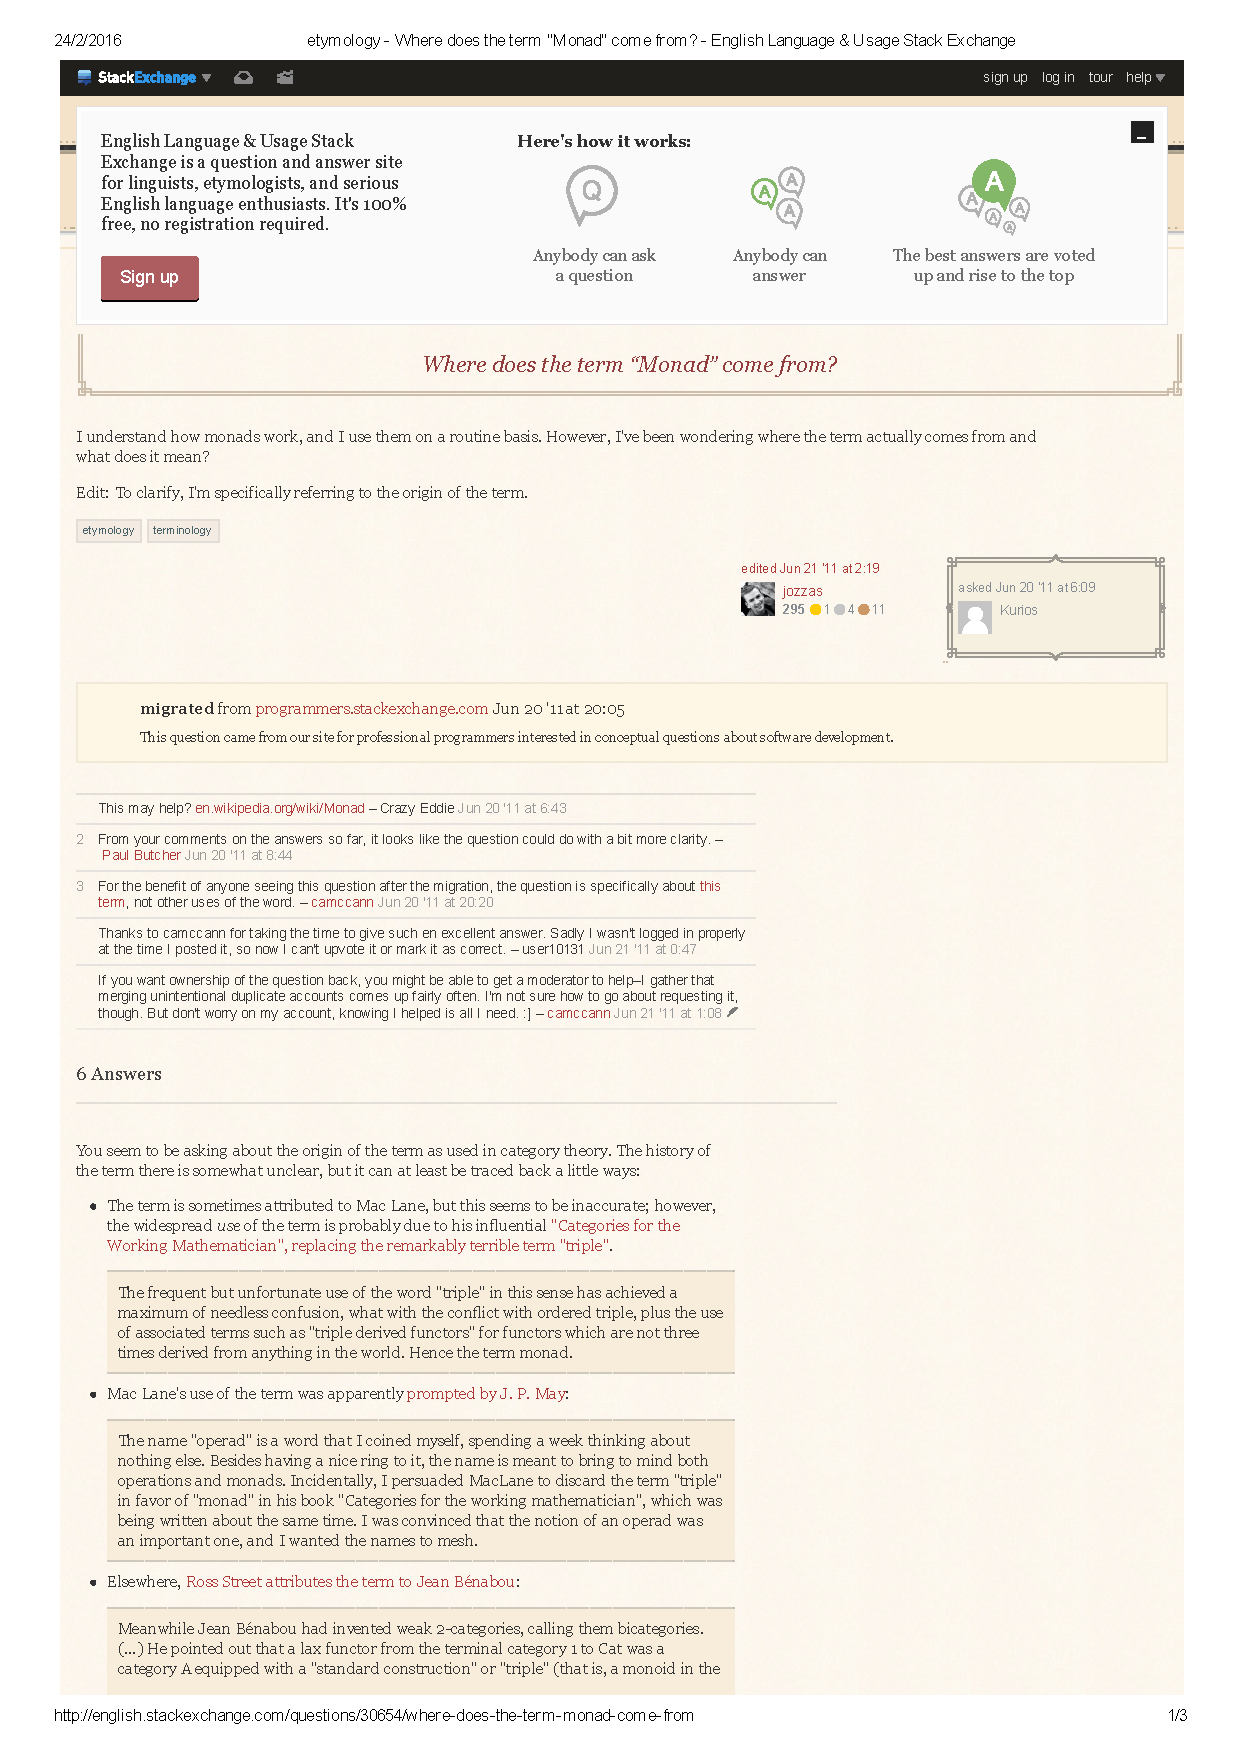
\includepdf[pages=-]{FAQ1.pdf}\cleardoublepage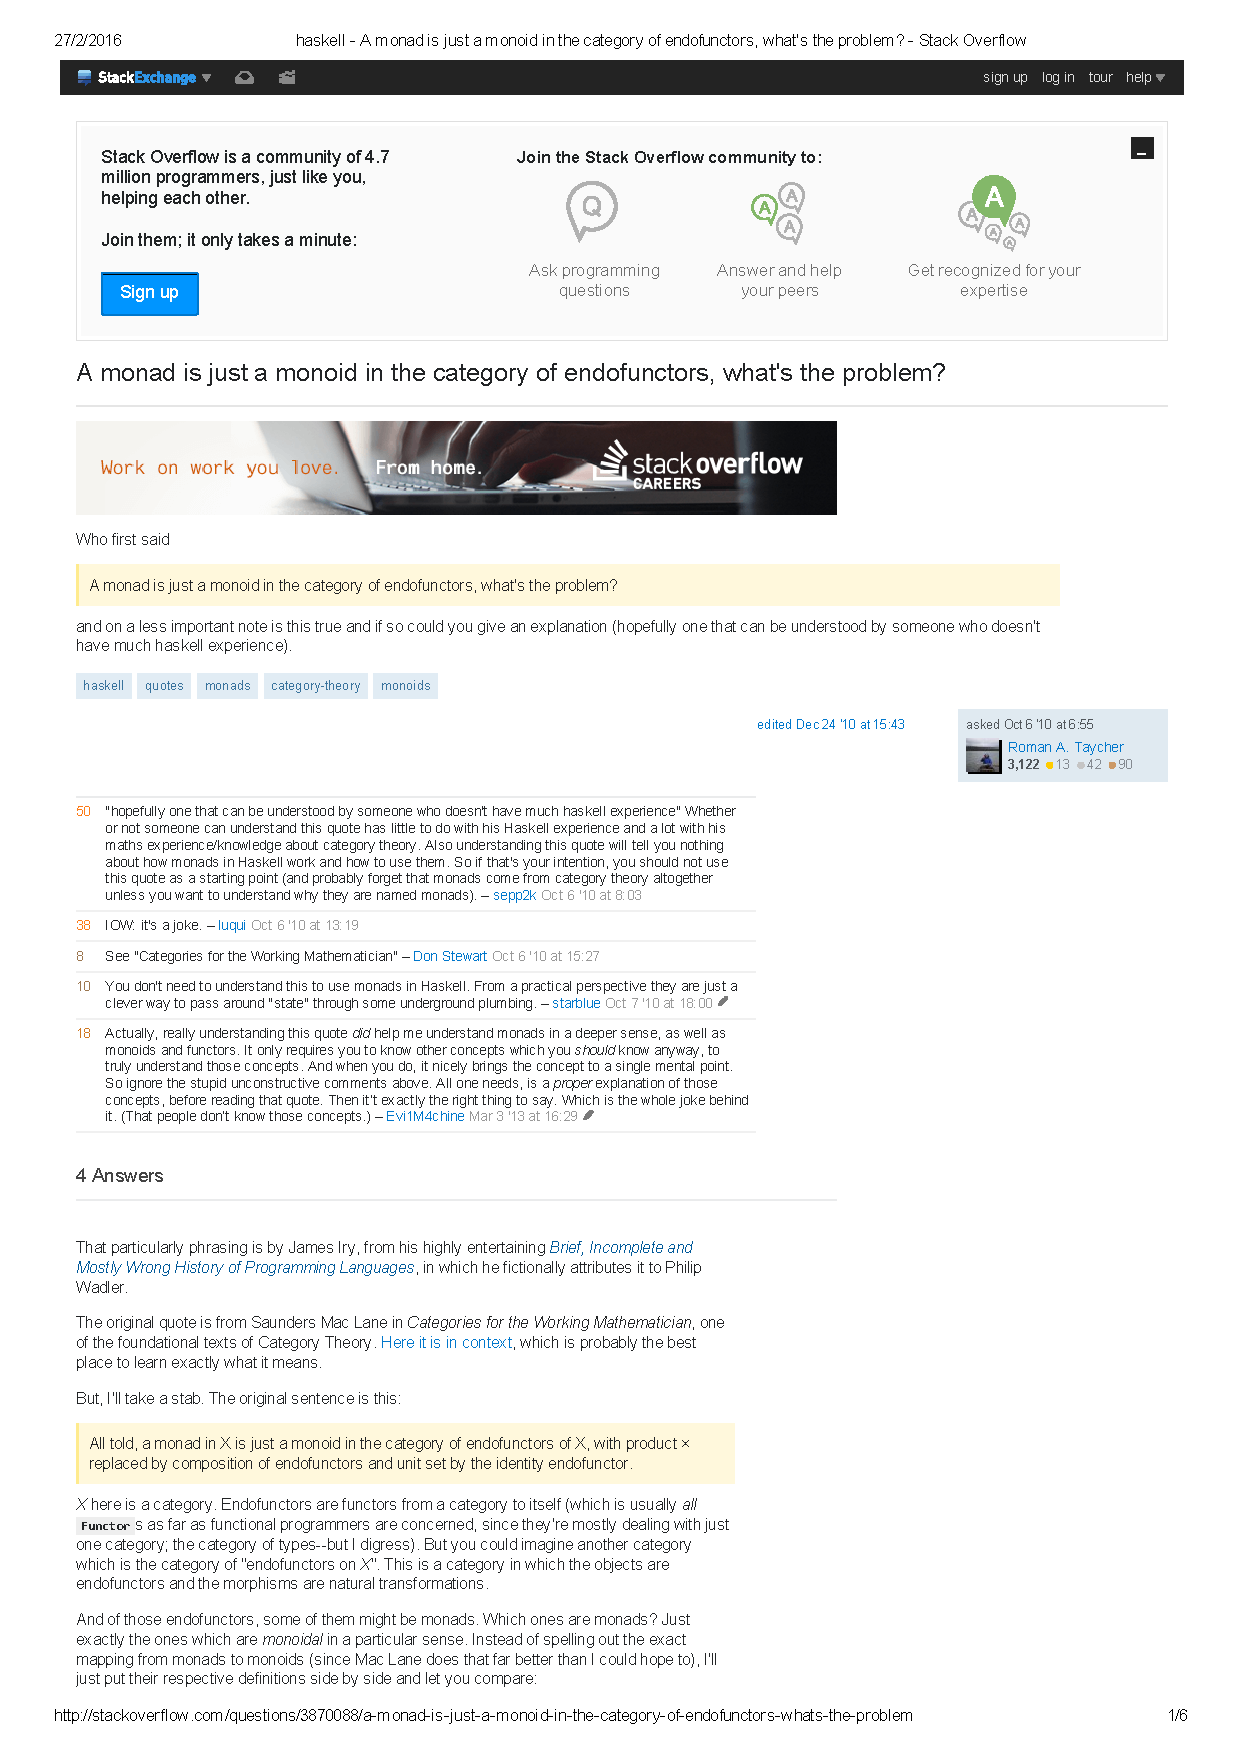
\includepdf[pages=-]{FAQ2.pdf}\cleardoublepage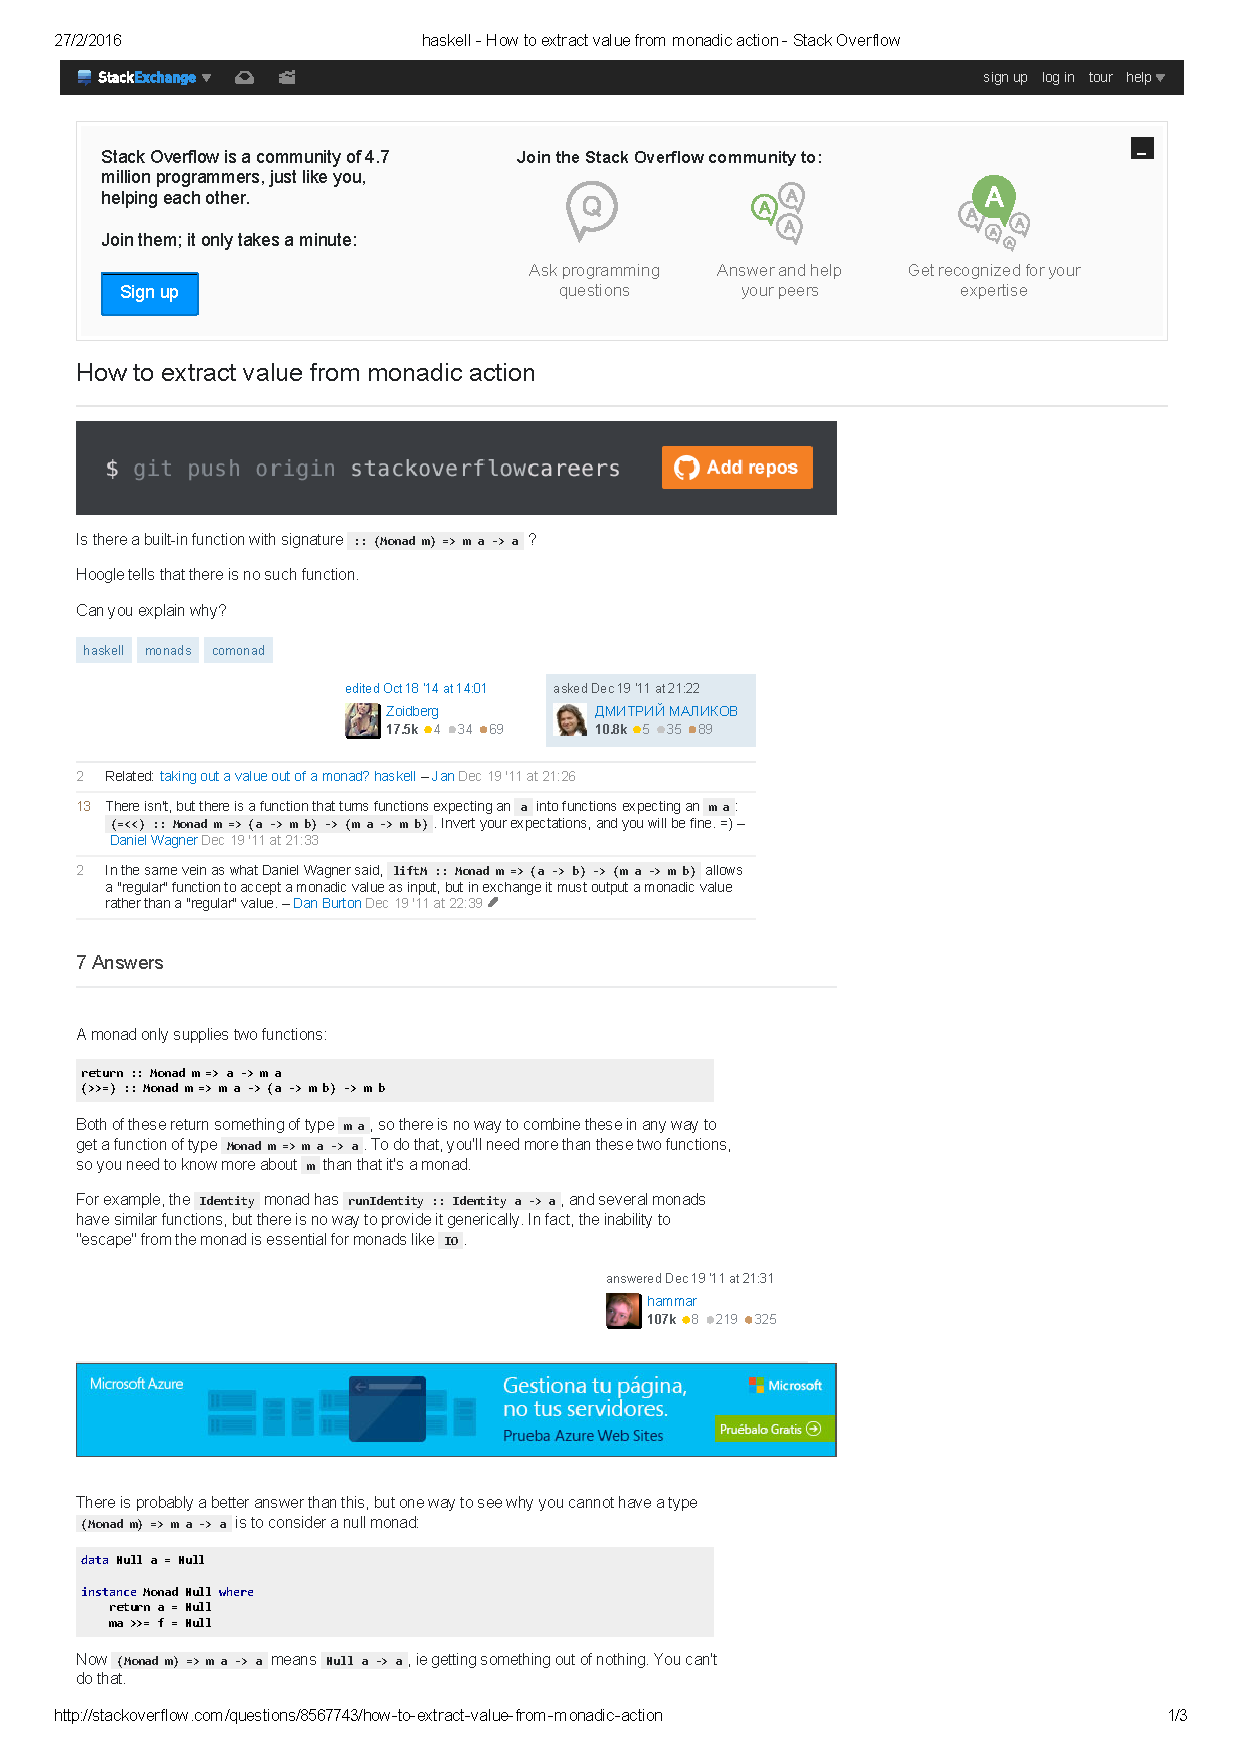
\includepdf[pages=-]{FAQ3.pdf}\cleardoublepage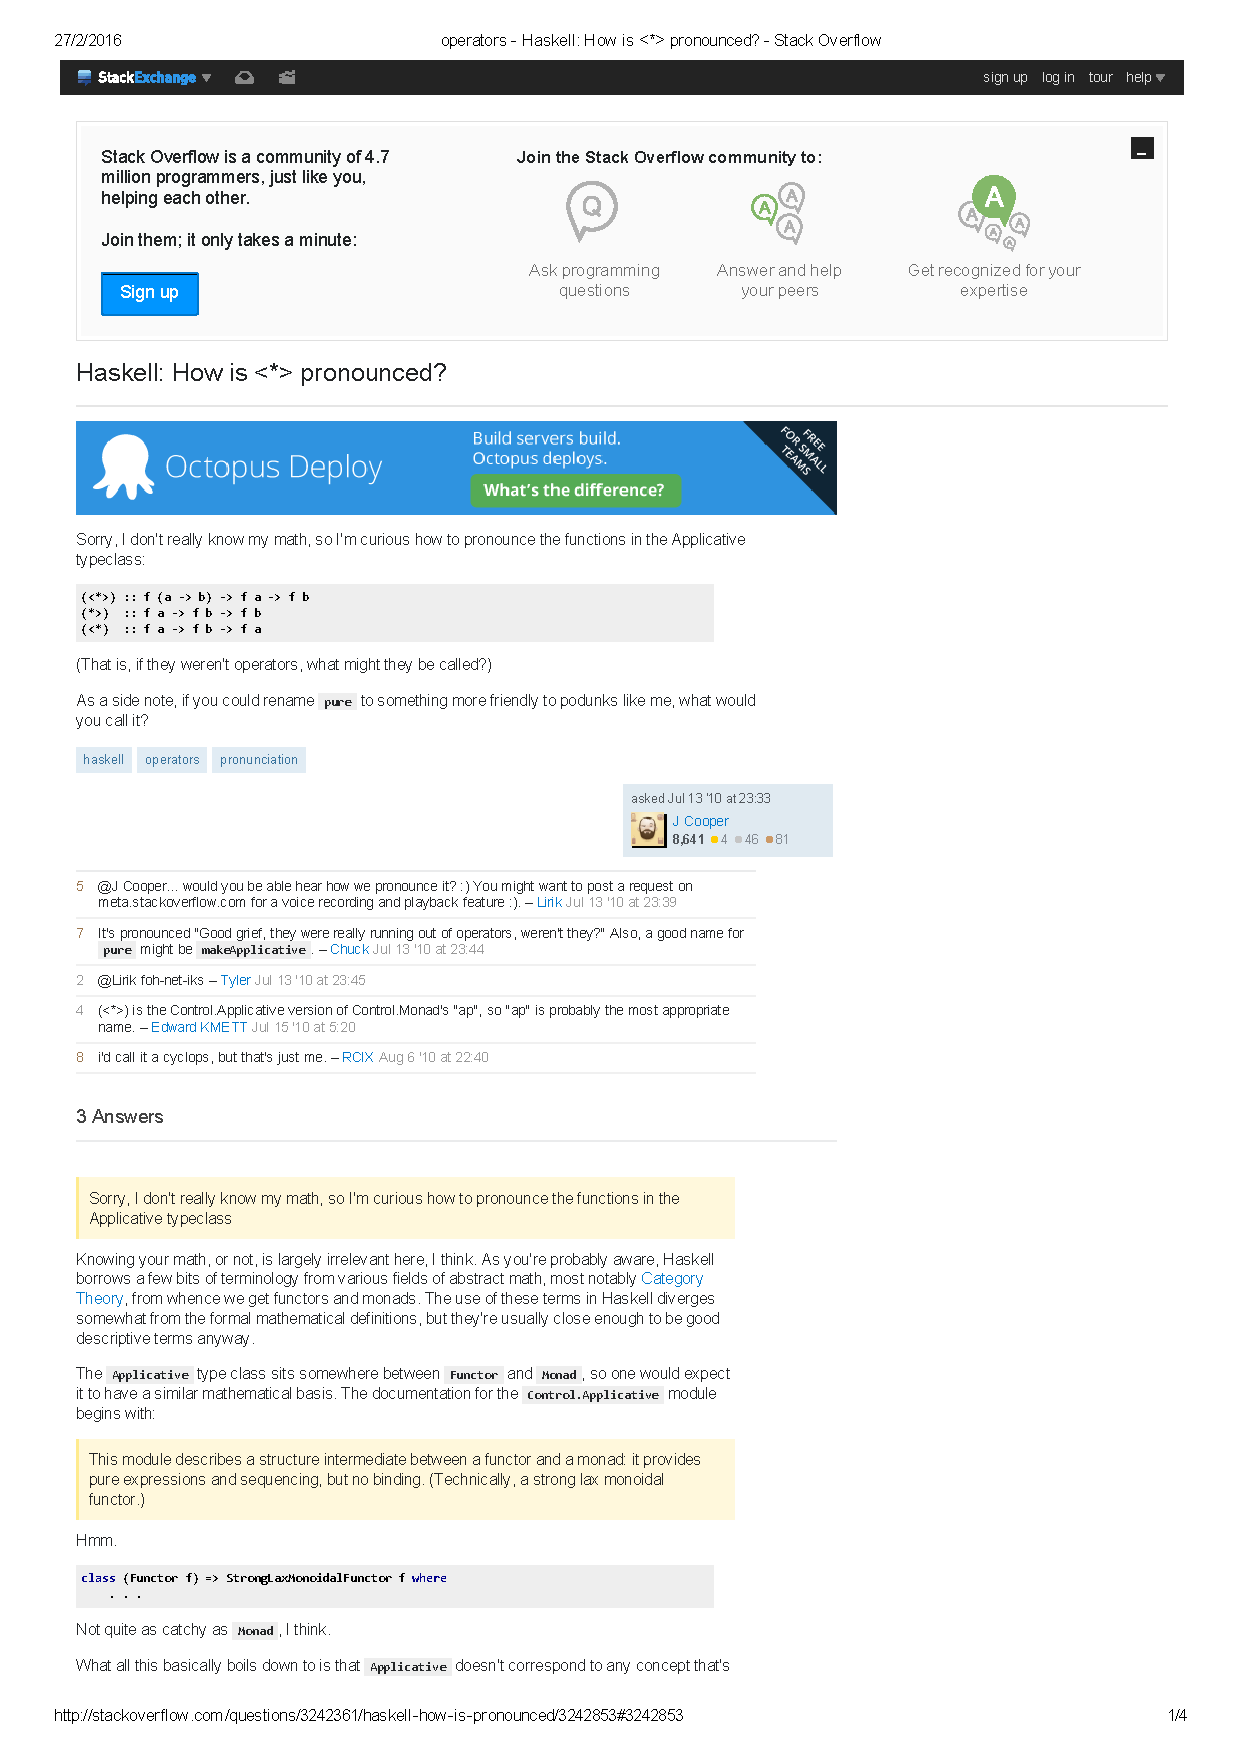
\includepdf[pages=-]{FAQ3-1.pdf}\cleardoublepage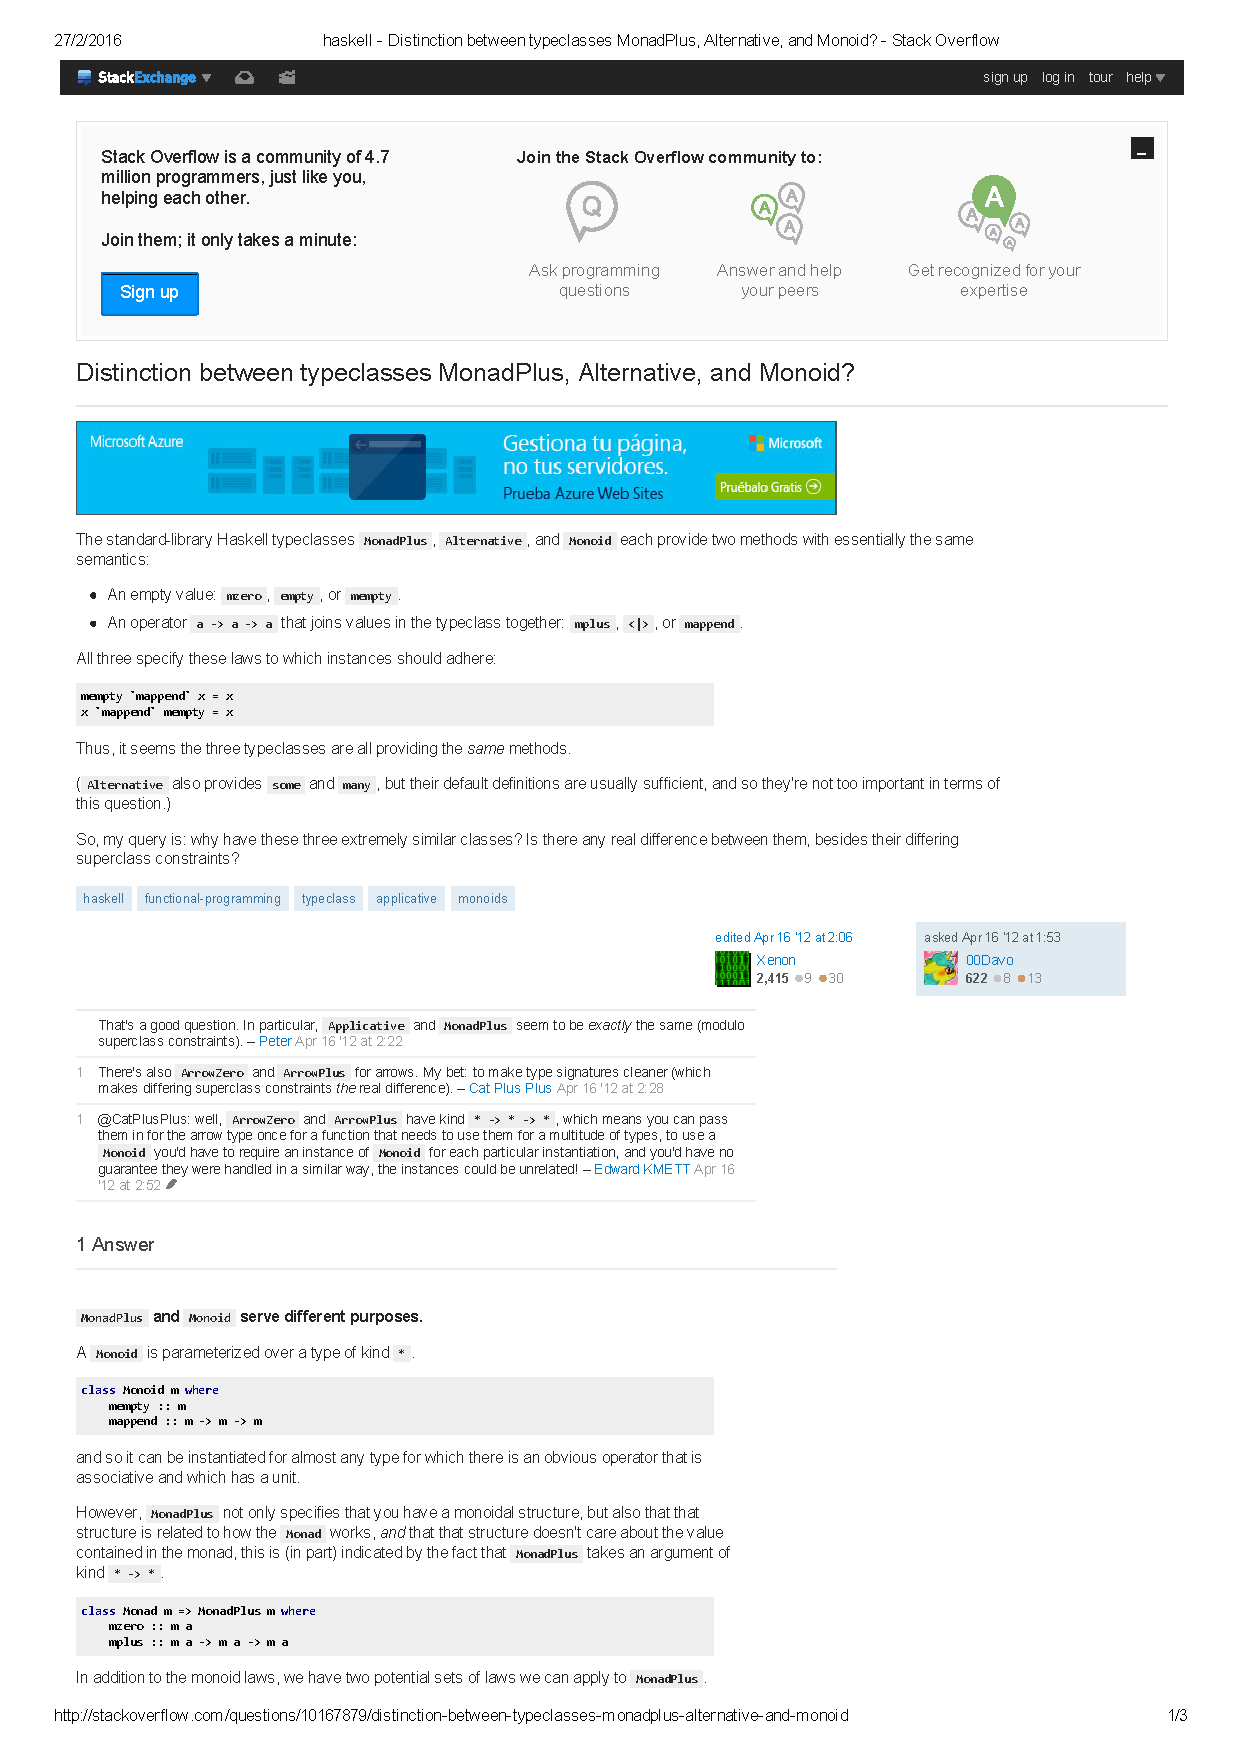
\includepdf[pages=-]{FAQ4.pdf}\cleardoublepage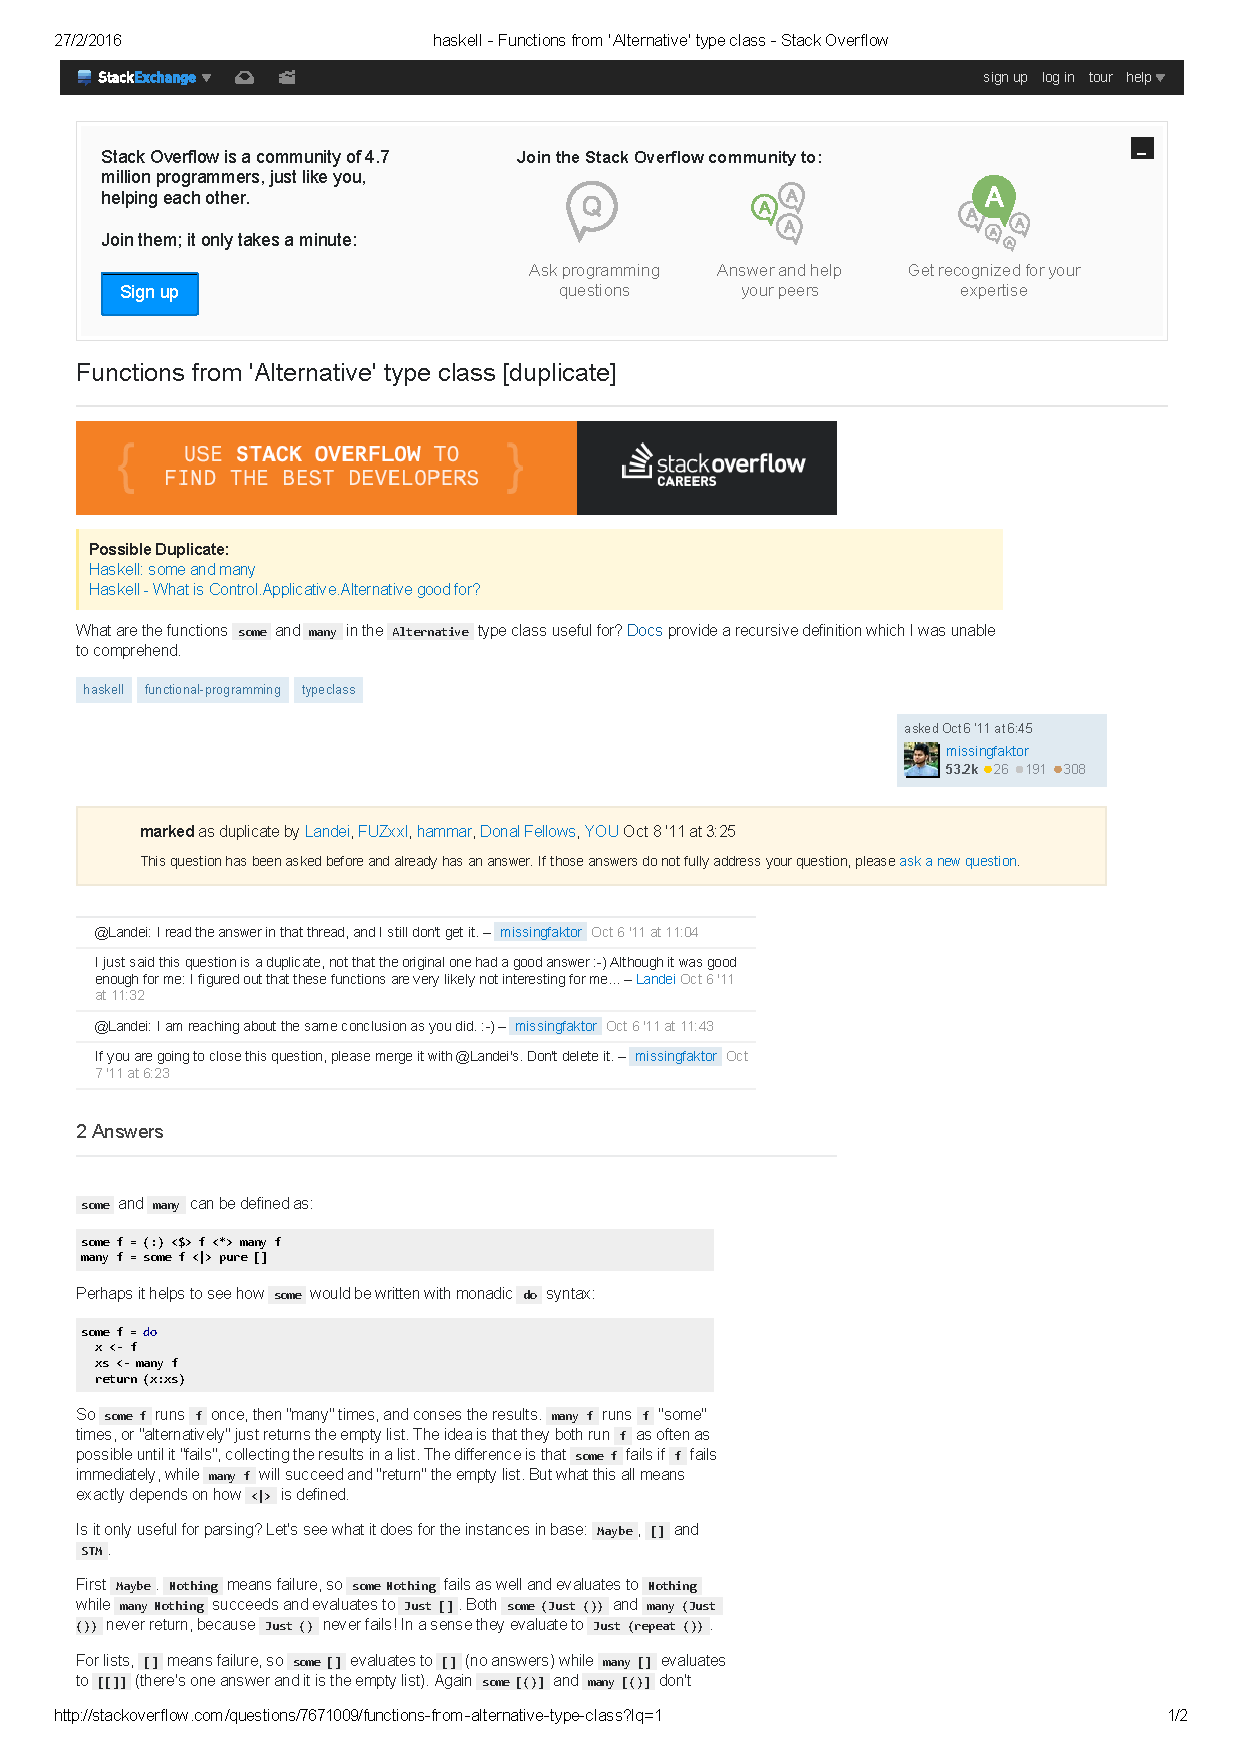
\includepdf[pages=-]{FAQ5.pdf}\cleardoublepage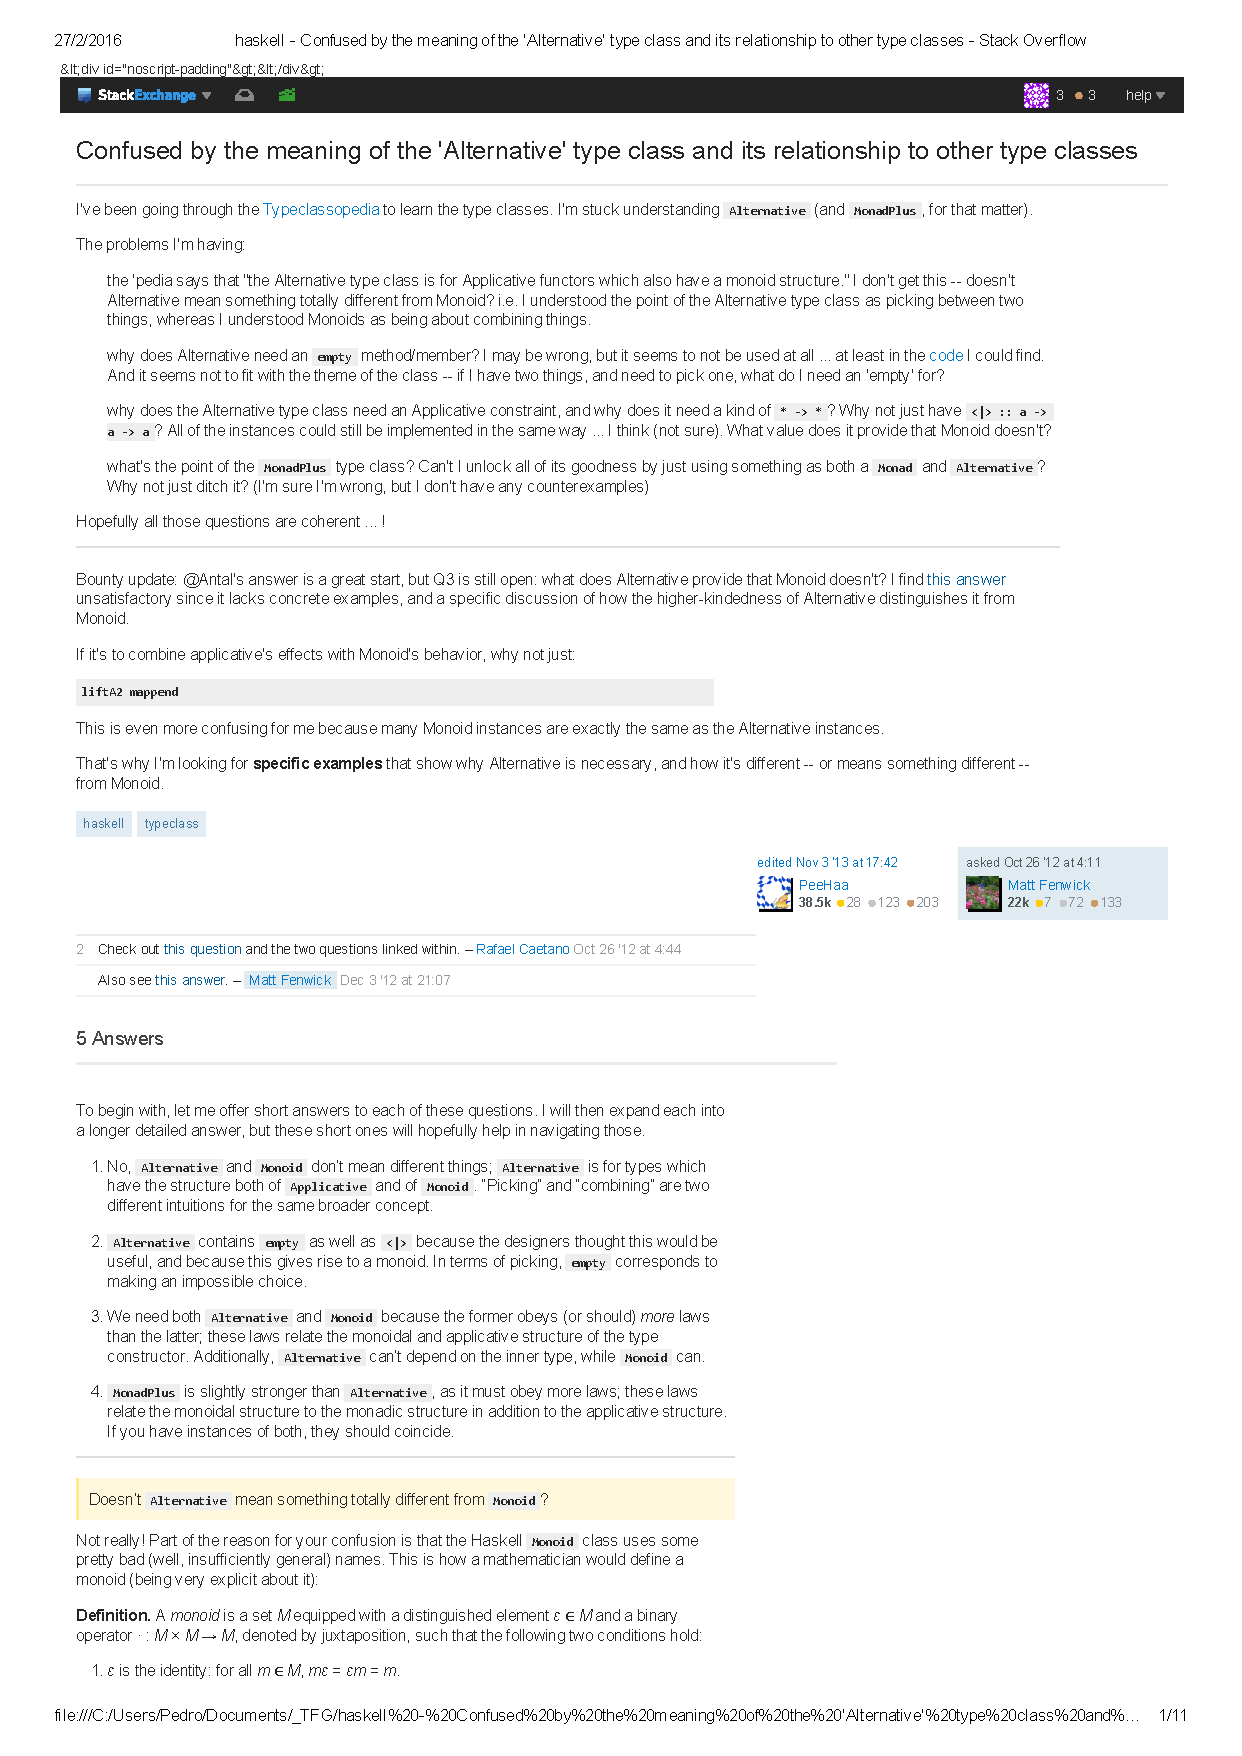
\includepdf[pages=-]{FAQ6.pdf}\cleardoublepage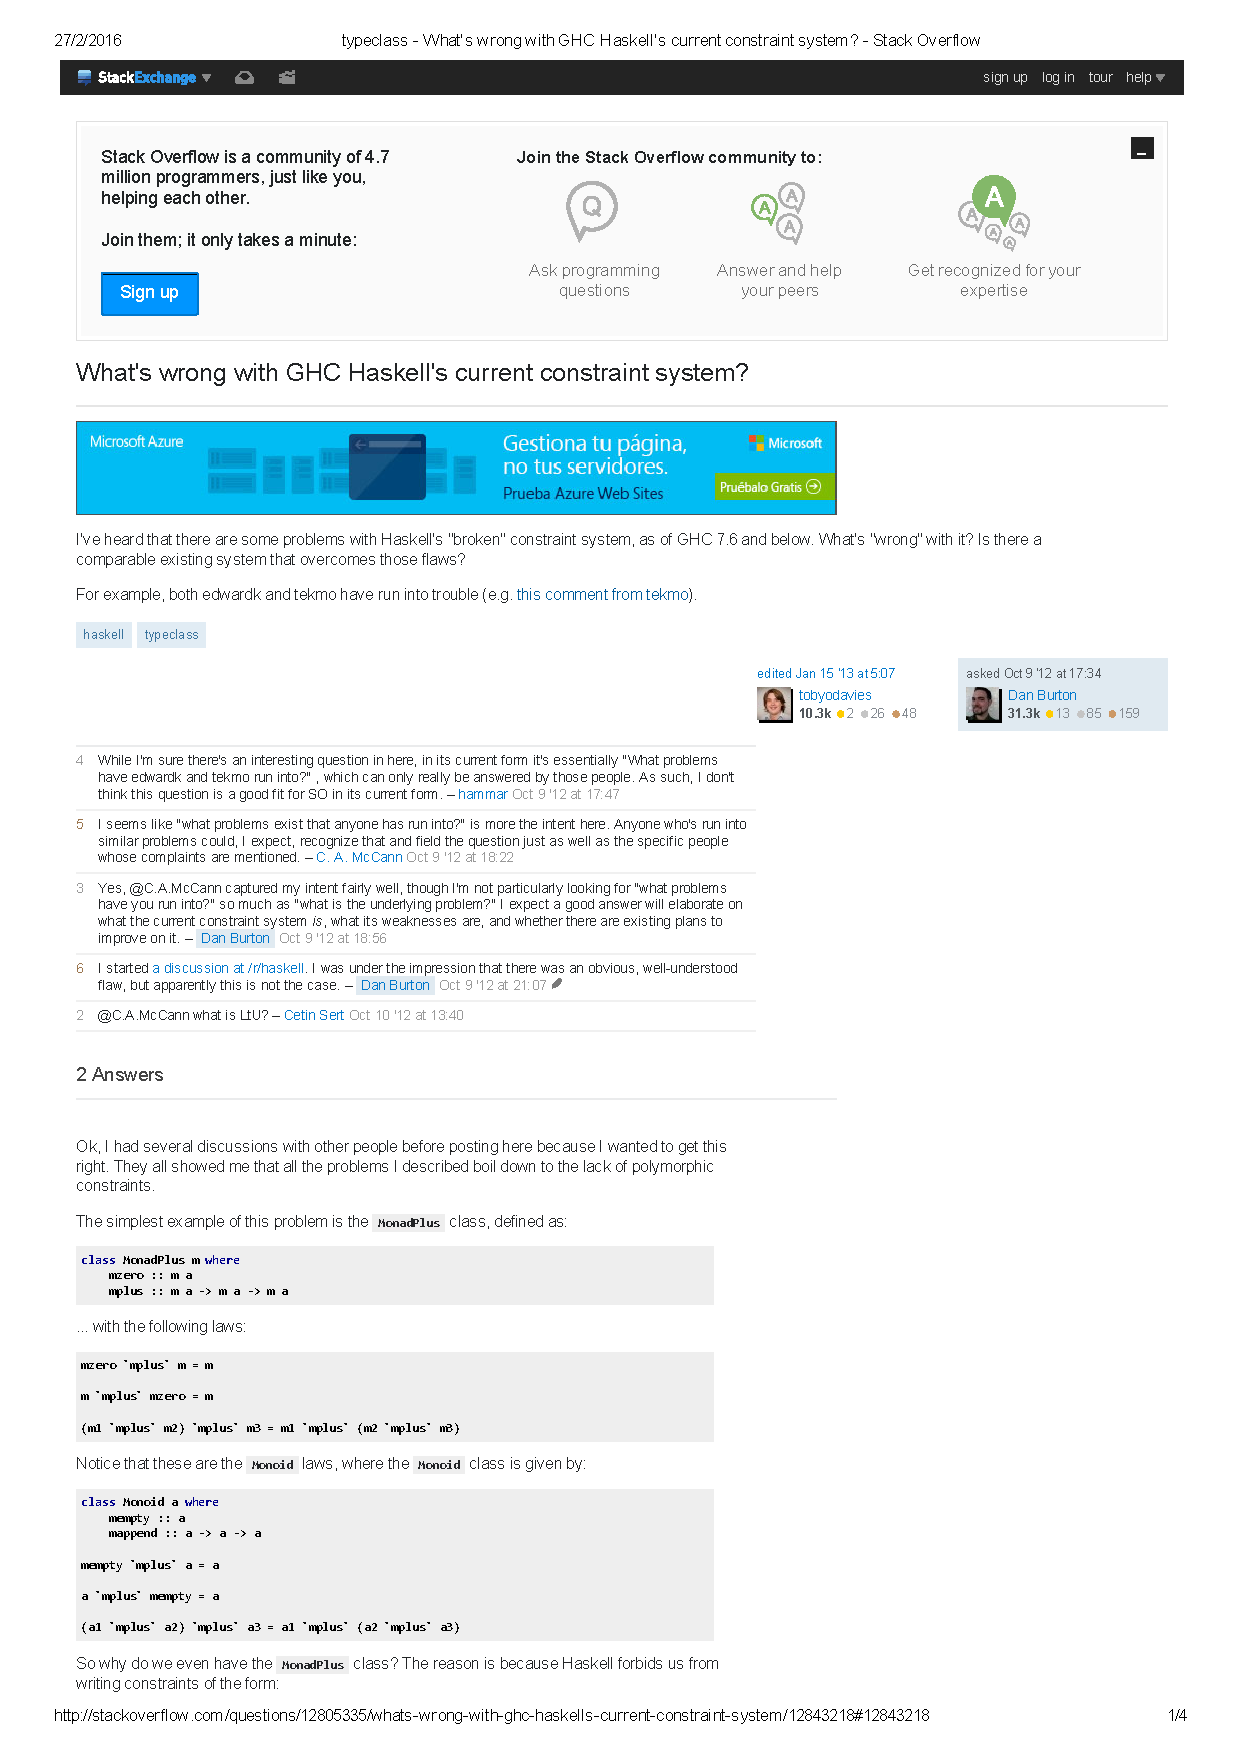
\includepdf[pages=-]{FAQ7.pdf}\cleardoublepage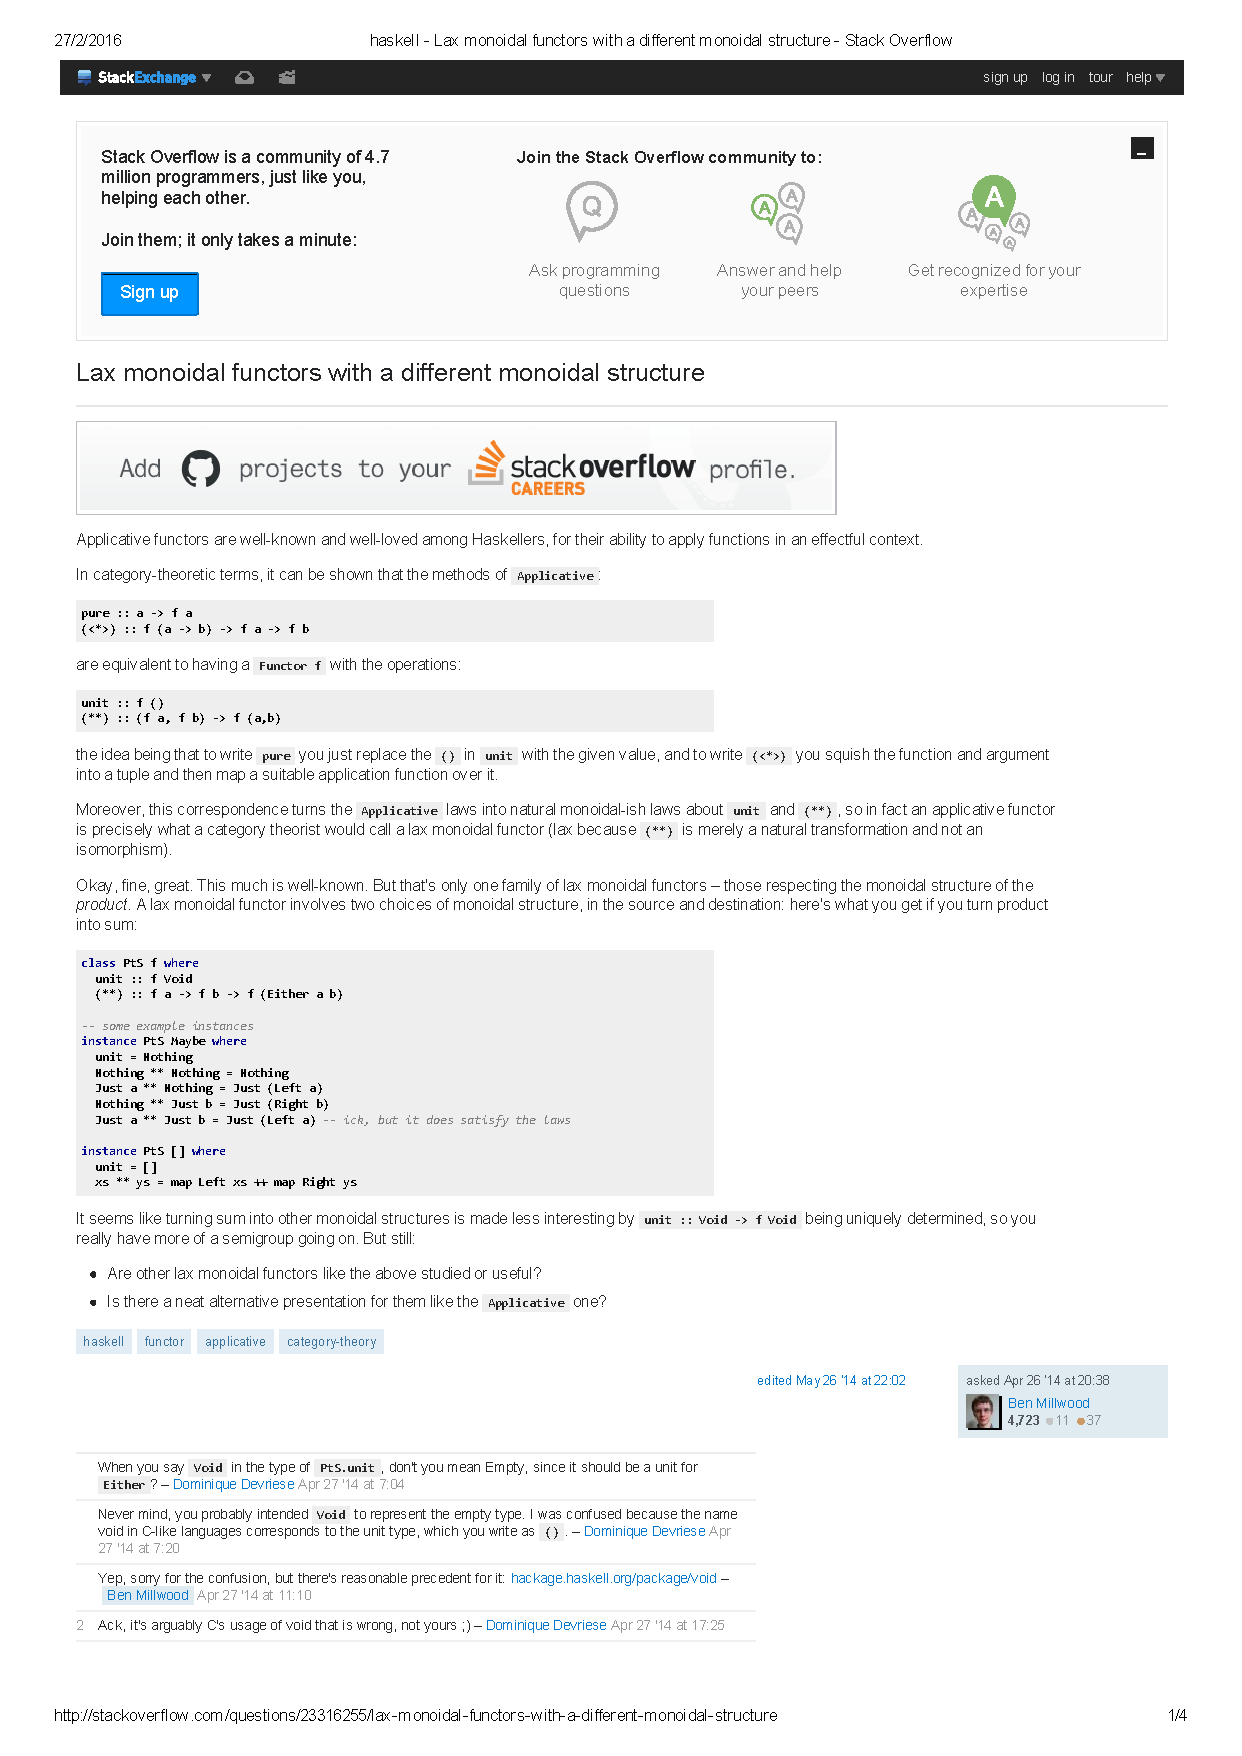
\includepdf[pages=-]{FAQ8.pdf}\cleardoublepage\end{document}